\documentclass{beamer}

\usepackage[beamer]{shortcut}

\usepackage{amsfonts}


\usepackage{array}
\usepackage{xcolor,colortbl}
\newcolumntype{a}{ >{\columncolor{blue}} c }

\usepackage{tikz}
\usepgflibrary{shapes.arrows}

\graphicspath{{./images/}}

\institute{INRIA Saclay}
\author{Thomas Moreau}
\title{
    Machine Learning and Modeling for Neural Data
}

\setbeamertemplate{title page}[frame]
\def\extraLogo{}

\newcommand{\citeline}[1]{\textcolor{gray}{\small[{\color{linkcolor} #1}]}}
\newcommand{\blue}[1]{\textcolor{blue}{#1}}
\newcommand{\red}[1]{\textcolor{red}{#1}}


\def\biblio{
	\nobibliography{library}
	\def\biblio{}
}

\begin{document}

    \begin{frame}
        \titlepage
    	\biblio{}
    \end{frame}


\begin{frame}{Gait analysis}

    \begin{columns}[T]
        \column{.58\textwidth}
        \centering
            \begin{columns}[c]
                \column{.4\linewidth}
                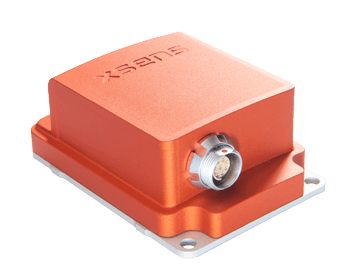
\includegraphics[width=\linewidth]{xsens}
                \column{.6\linewidth}
                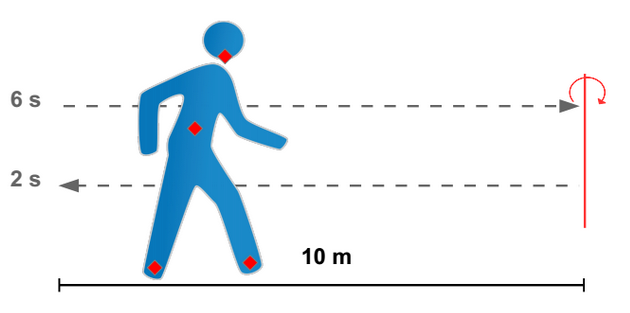
\includegraphics[width=\linewidth]{exo_marche}
            \end{columns}
            {\tiny Healthy subject record (Hôpital Militaire de Percy)}
            \only<1>{%
                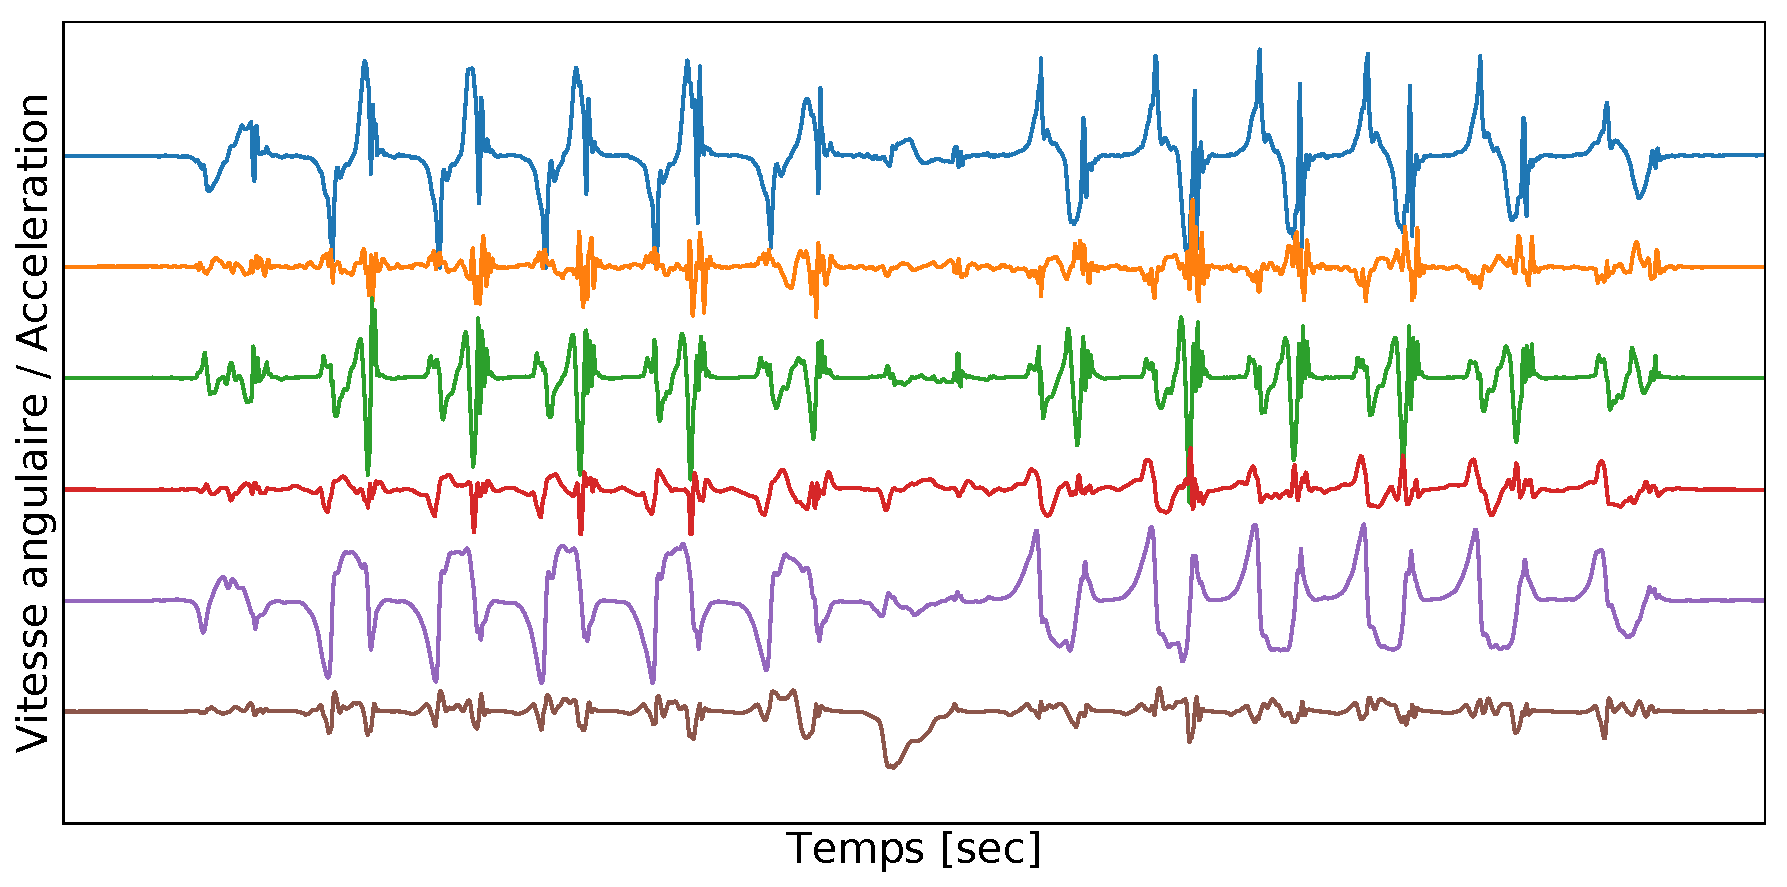
\includegraphics[width=\linewidth]{accelero}
            }
            \only<2-3>{%
                \overimg[\linewidth]{2}{accelero_steps}{3}{accelero_dict}
            }
            \vskip-1em\hskip.5ex
            \begin{beamercolorbox}[rounded=true, shadow=true, wd=.95\linewidth]{title}
                \textbf{Patent:~} \textcolor{black}{Step Segmentation}\\
                \textbf{Articles:} %
                    \textcolor{linkcolor}{Sensors 2018; PLoS One 2016}\\
            \end{beamercolorbox}
        \column{.4\textwidth}
                \begin{block}{\bf Quantifying Equilibrium}
                    \vskip.5em
                    \begin{itemize}\itemsep.5em
                        \item Fall prediction
                        \item Neuropathy follow up
                    \end{itemize}
                    \vskip-.7em\textcolor{white}{.}
                \end{block}
                \begin{block}{\bf Challenges}
                    \vskip.3em
                    Few annotations\\[.5em]
                    How to compare signals?
                    \vskip-.7em\textcolor{white}{.}
                \end{block}
                \begin{block}{\bf Signals Comparison}
                    \vskip.5em
                    Adapted representation\\[.5em]
                    {\bf Local Structures} $\Rightarrow$ steps
                    \vskip-.7em\textcolor{white}{.}
                \end{block}
        \end{columns}

    \end{frame}

\frame{
    \frametitle{Studying the Nystagmus}
{\centering
\begin{columns}
    \column{.59\textwidth}
    \only<1>{
        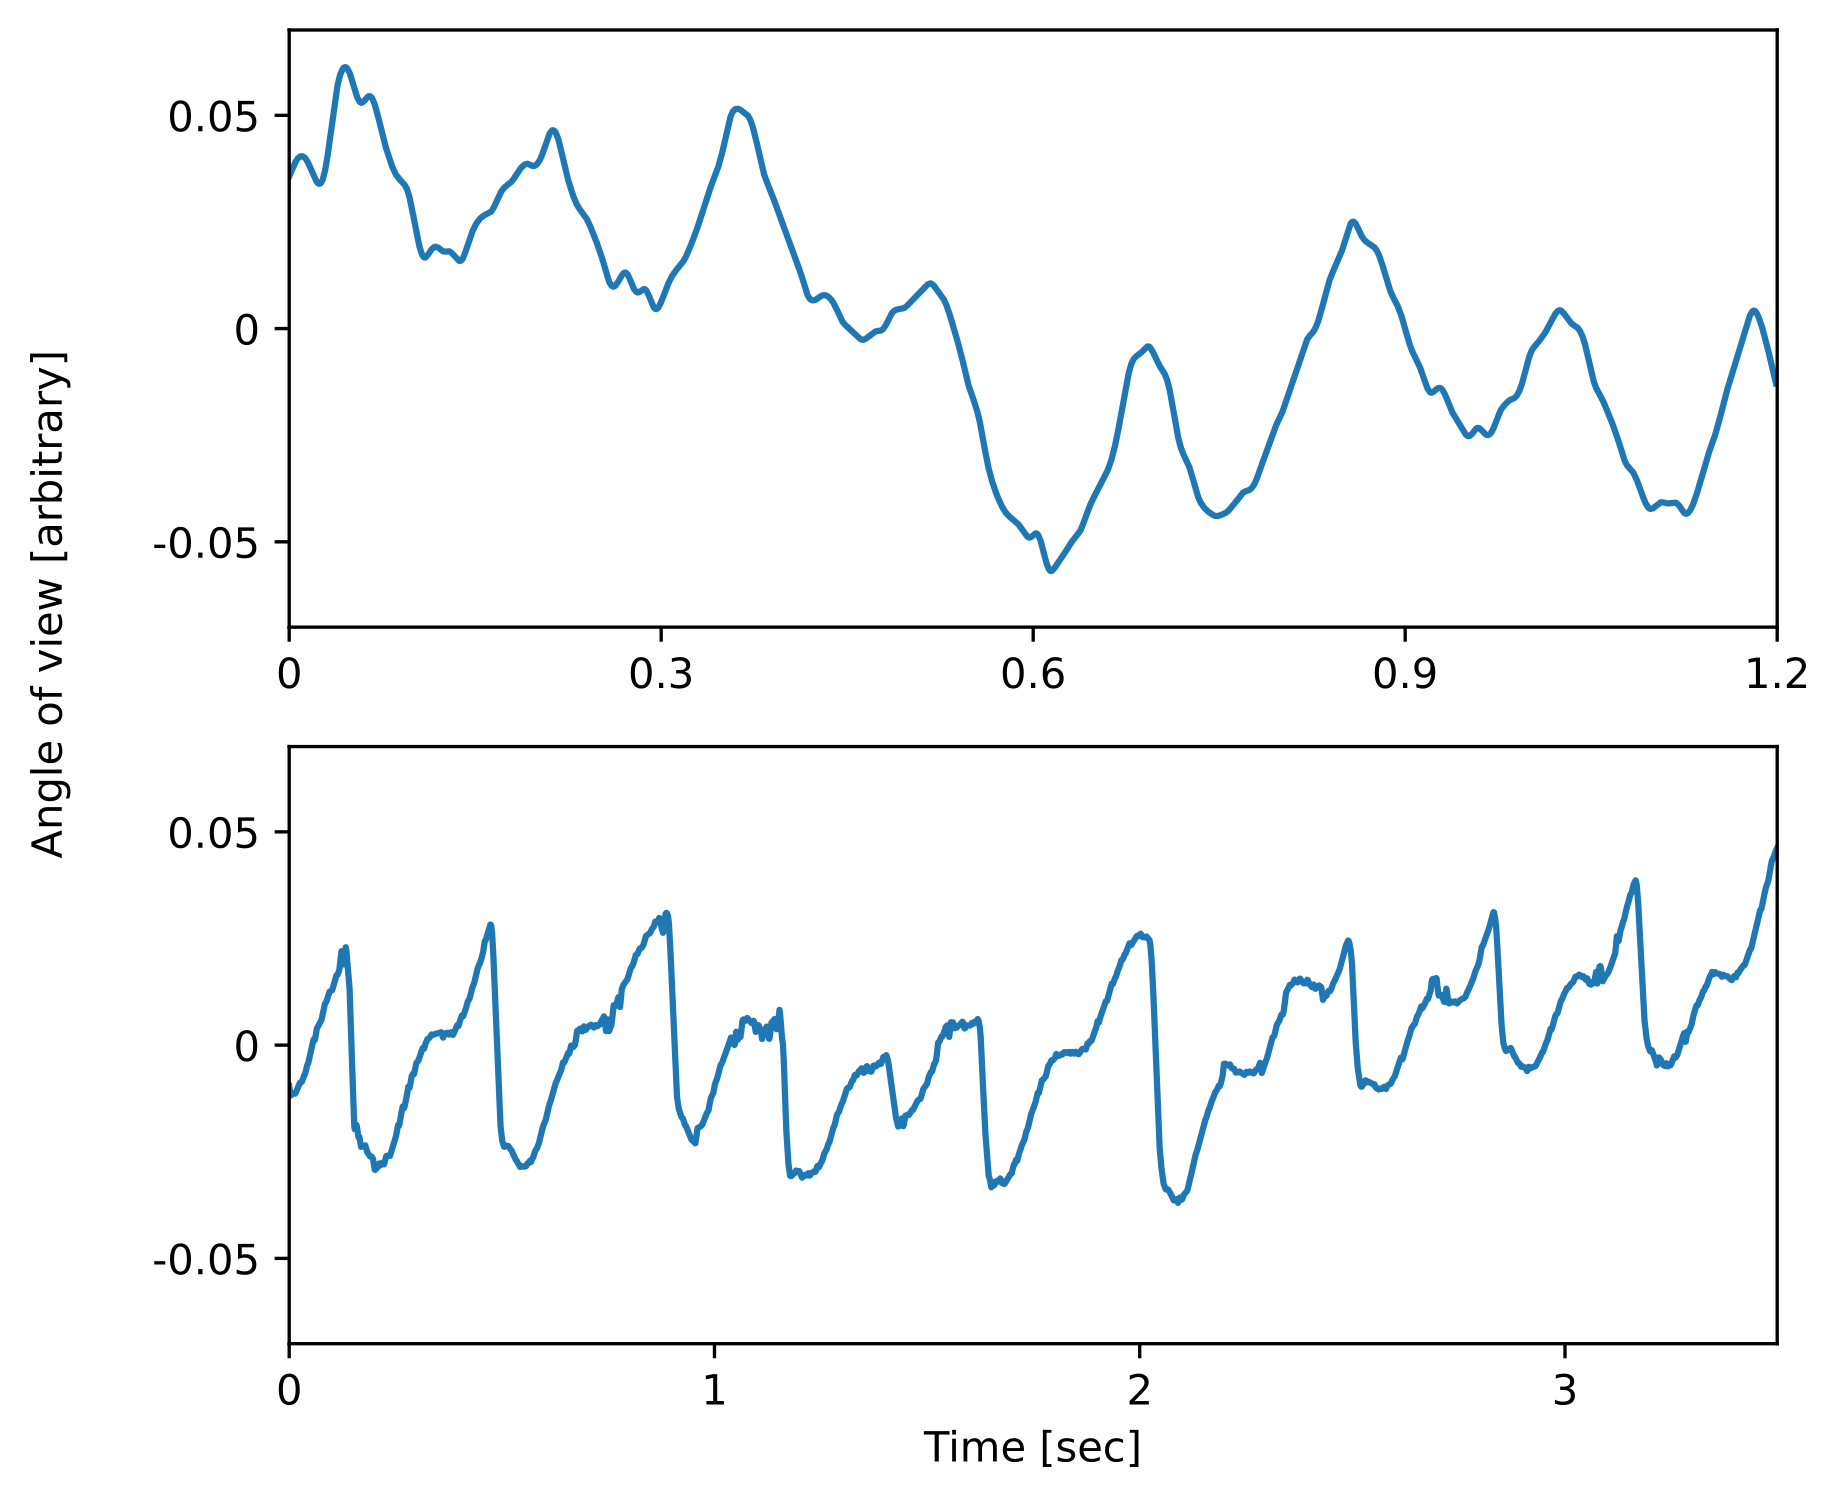
\includegraphics[width=\textwidth]{oculo_signal.png}
    }
    \only<2->{
        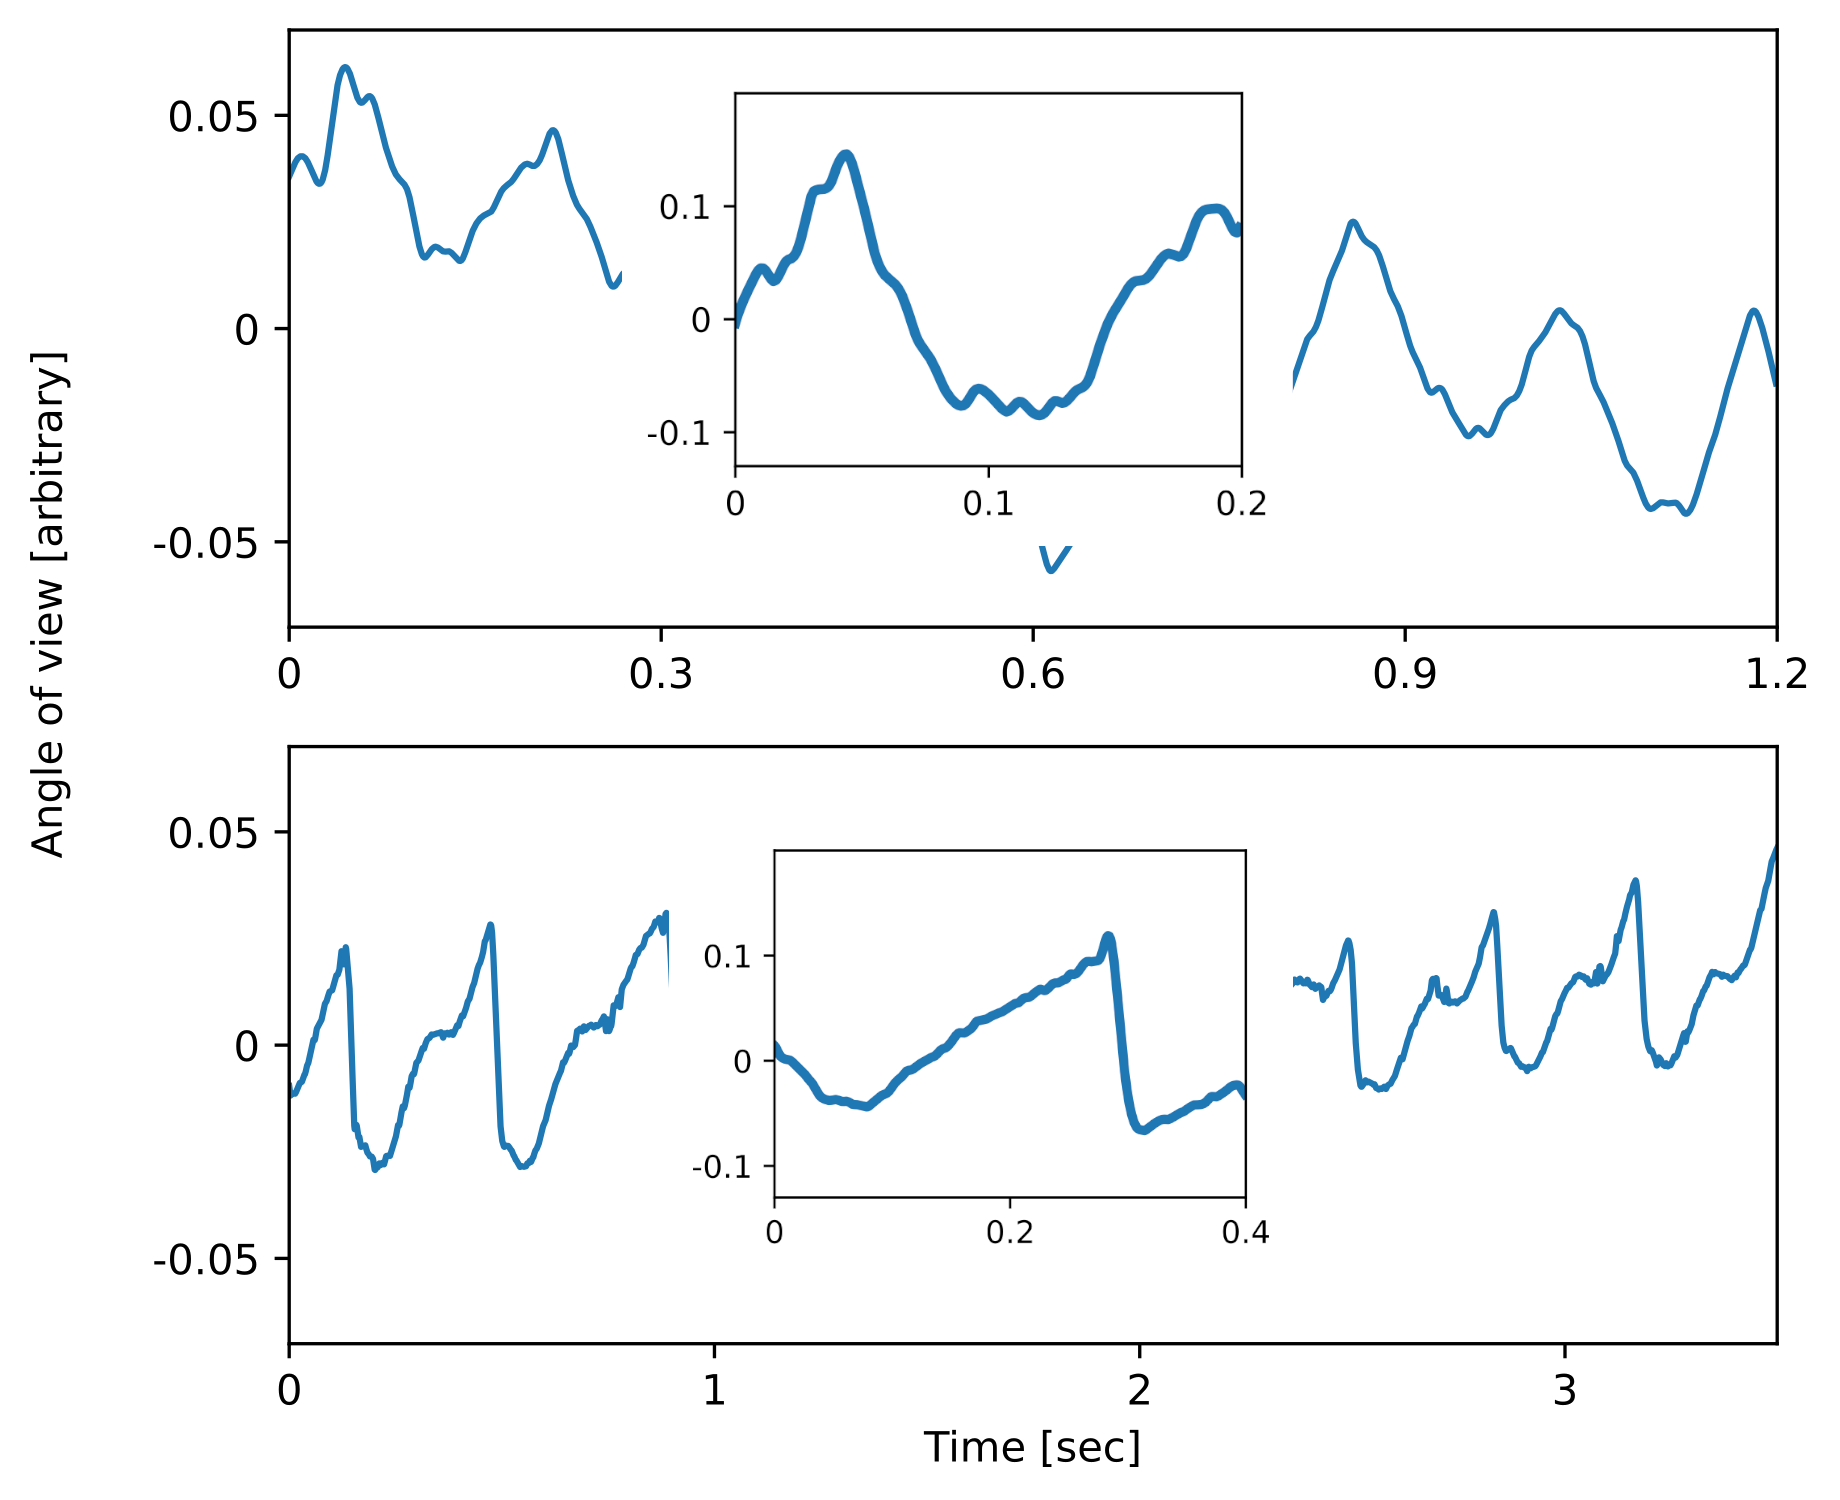
\includegraphics[width=\textwidth]{oculo_signal_dict.png}
    }\\

    \column{.39\textwidth}
    \centering
    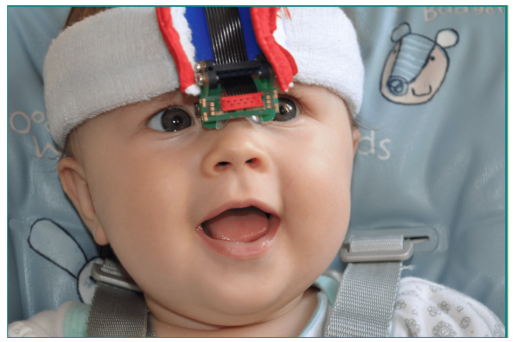
\includegraphics[width=.8\textwidth]{eyefant}\\
\end{columns}
}
}

\frame{
    \frametitle{Context: functional Neuroimaging}

    \large {\bf Goal:}
    Study the brain mechanisms while it is functioning.\\[3em]

    {\bf Outputs:}\\[1em]
    \begin{itemize}\itemsep1em
        \item {\bf Functional Atlases:} Link areas of the brain to specific cognitive functions.
        \item {\bf Functional Connectivity:} Highlight the information flow in the brain.
        \item {\bf Healthcare:} Develop bio-markers for neurological disorders.
    \end{itemize}
}

\frame[t]{
    \frametitle{Context: functional Neuroimaging}

    {\large How to record living brains electrical activity: \textbf{Electrophysiology}}\\[.3em]

    \centering\large Direct measurement: intracranial EEG.\\[.5em]
        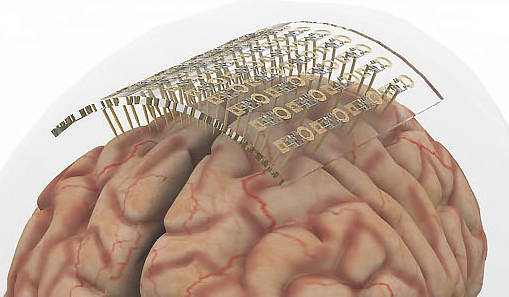
\includegraphics[width=.7\textwidth]{brain_probe.jpg}\\[1em]
        \begin{columns}
            \techterm{\color{darkblue} High Localization}%
            \techterm{Low Resolution}%
            \techterm{Invasive}%
        \end{columns}
}


\frame[t]{
    \frametitle{Context: functional Neuroimaging}

    {\large How to record living brains electrical activity: \textbf{Electrophysiology}}\\[.3em]

    \large\centering Remote measurement: M/EEG.\\[-.5em]
    \begin{columns}[T]
        \column{.35\textwidth}
        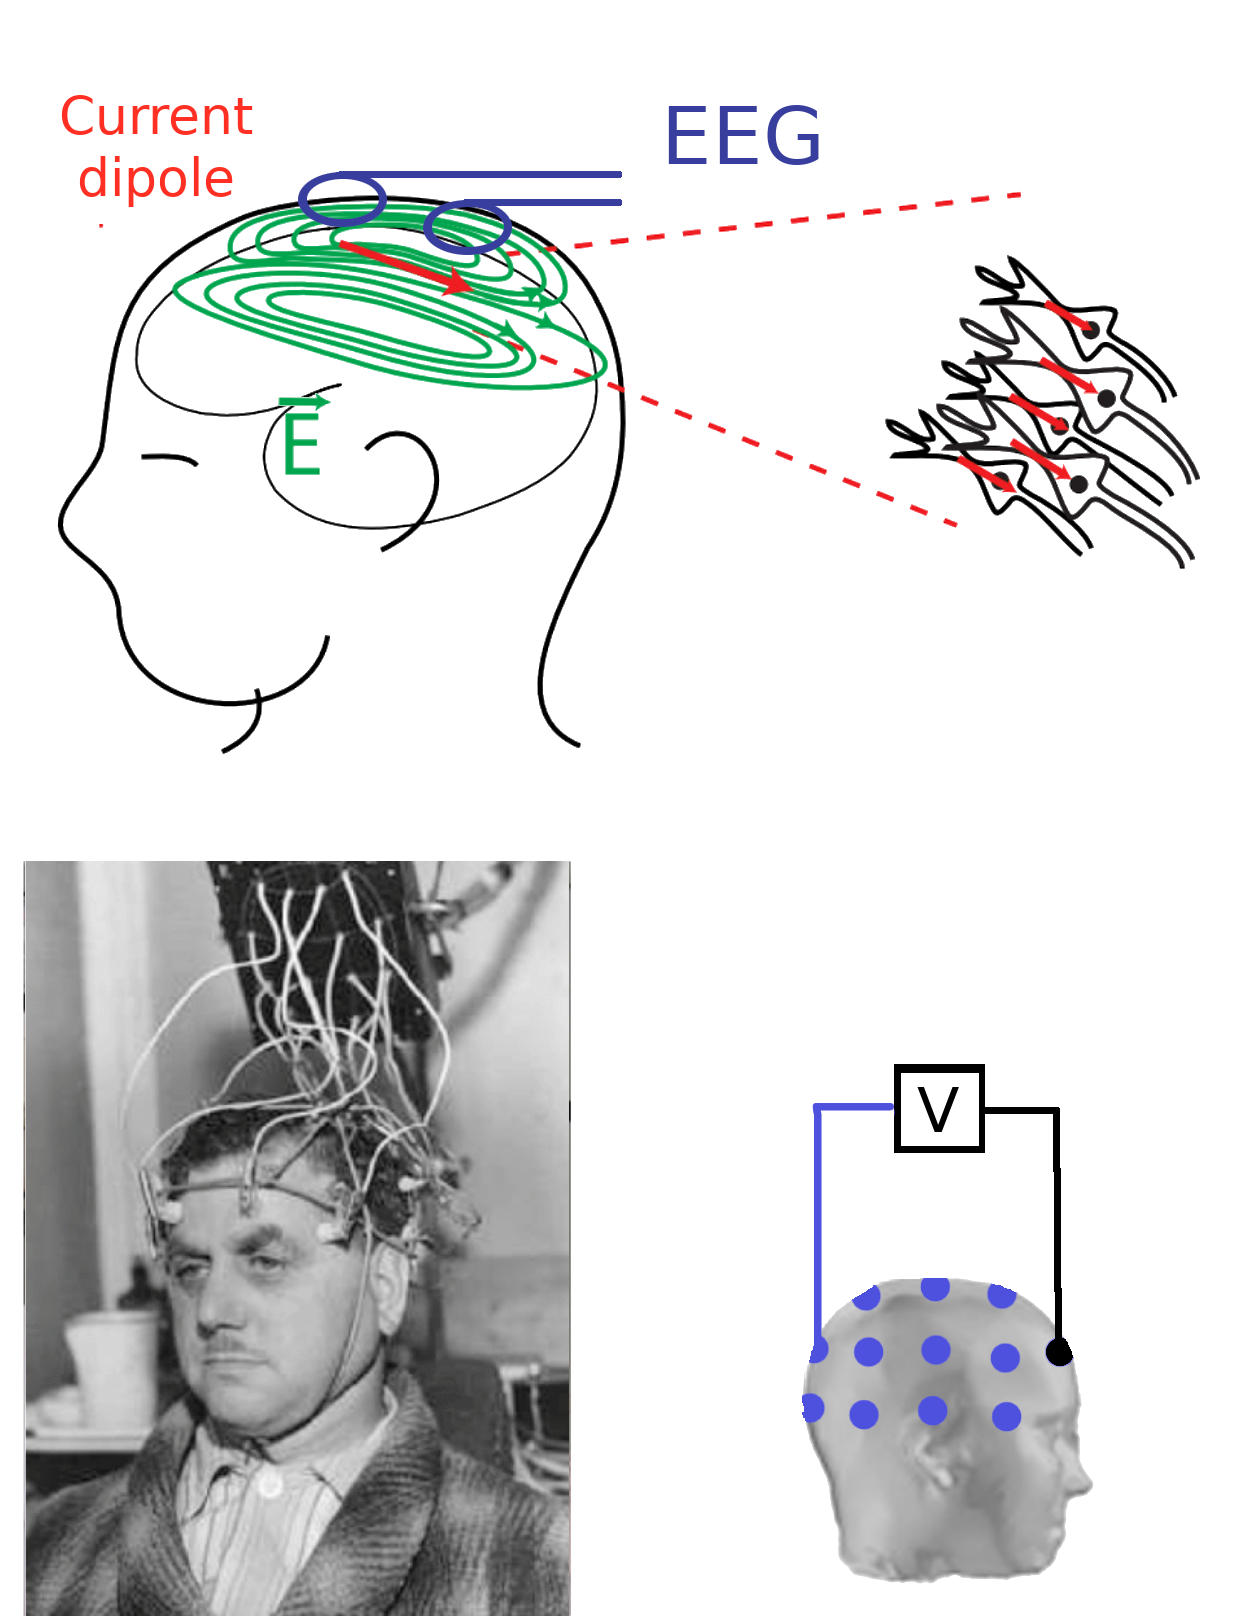
\includegraphics[width=\textwidth]{eeg_presentation}
        \column{.35\textwidth}
        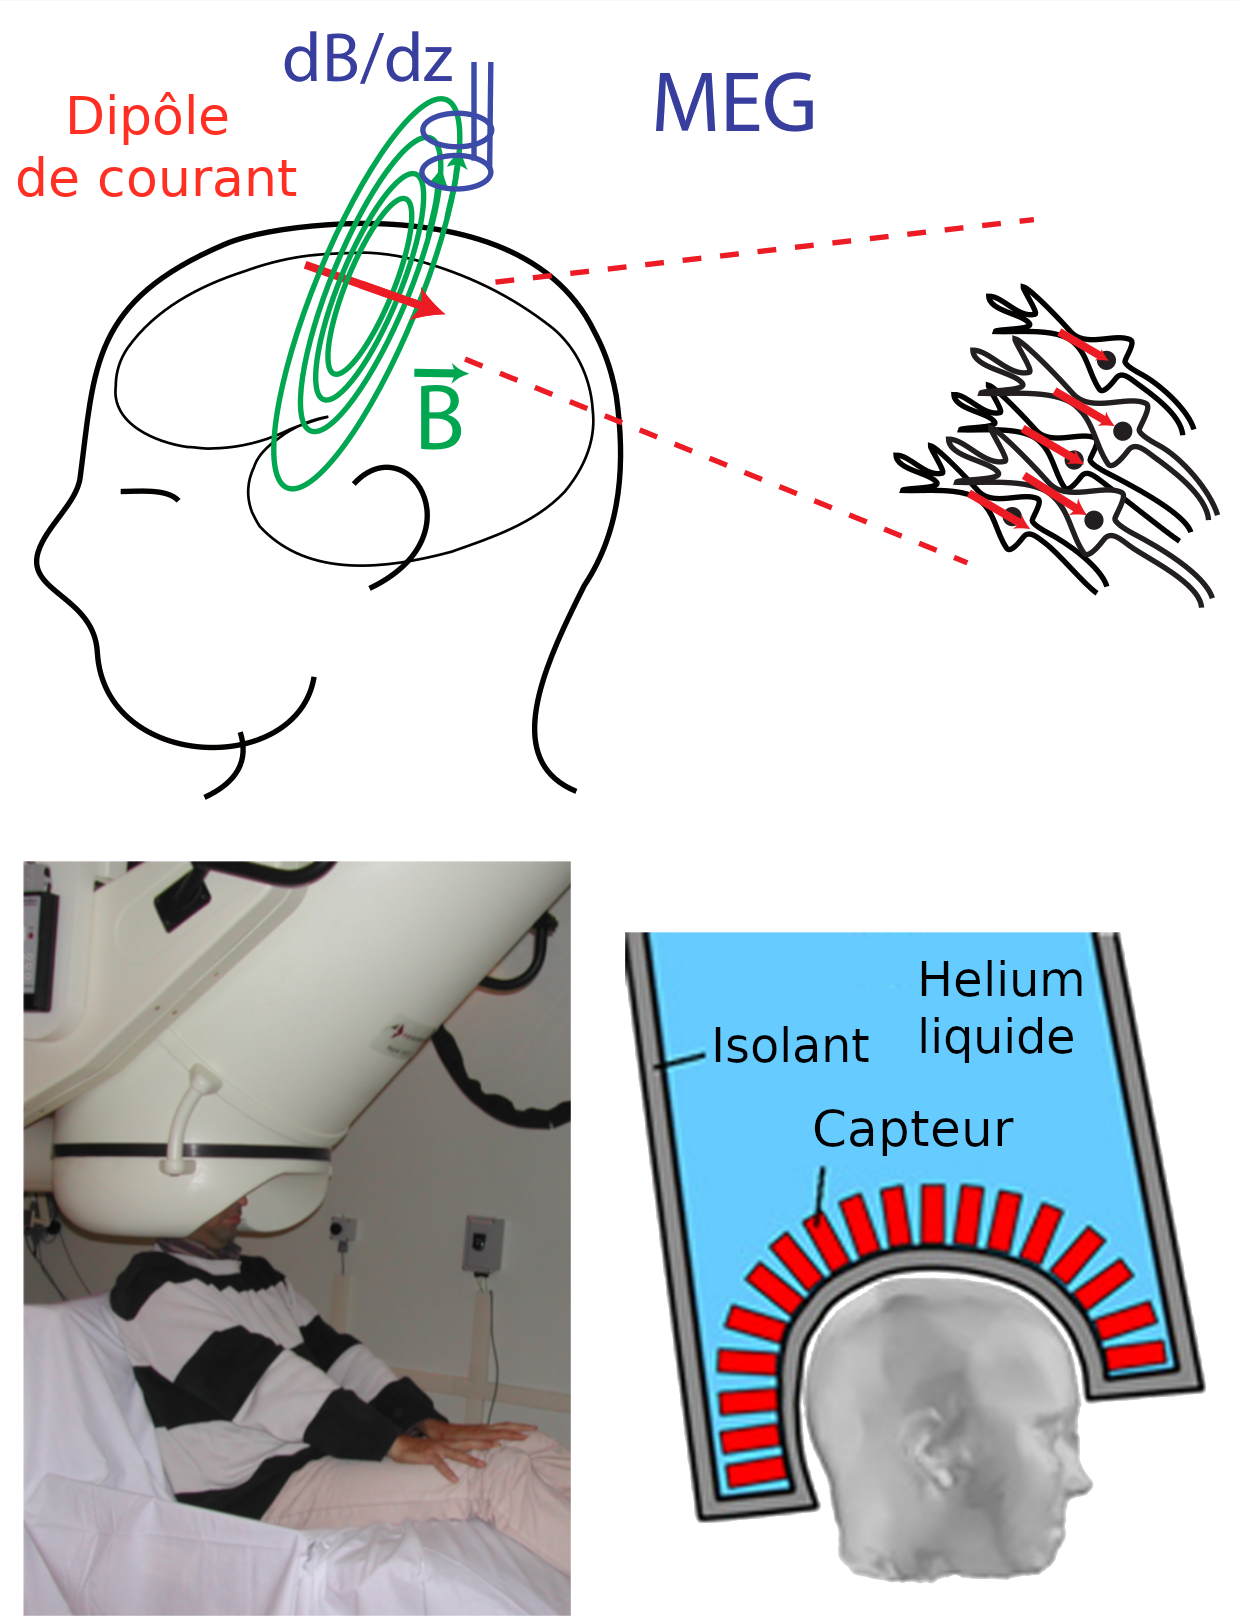
\includegraphics[width=\textwidth]{meg_presentation}
    \end{columns}
    % \only<2>{
    \begin{columns}
        \techterm{No Localization}%
        \techterm{\color{darkblue} Global}%
        \techterm{\color{darkblue} Non Invasive}%
    \end{columns}
    % }

}

\frame{
    \frametitle{M/EEG signals}

    {\Large\bf Multivariate time-series $X$}\\[1em]

    \centering
    \alt<3>{
        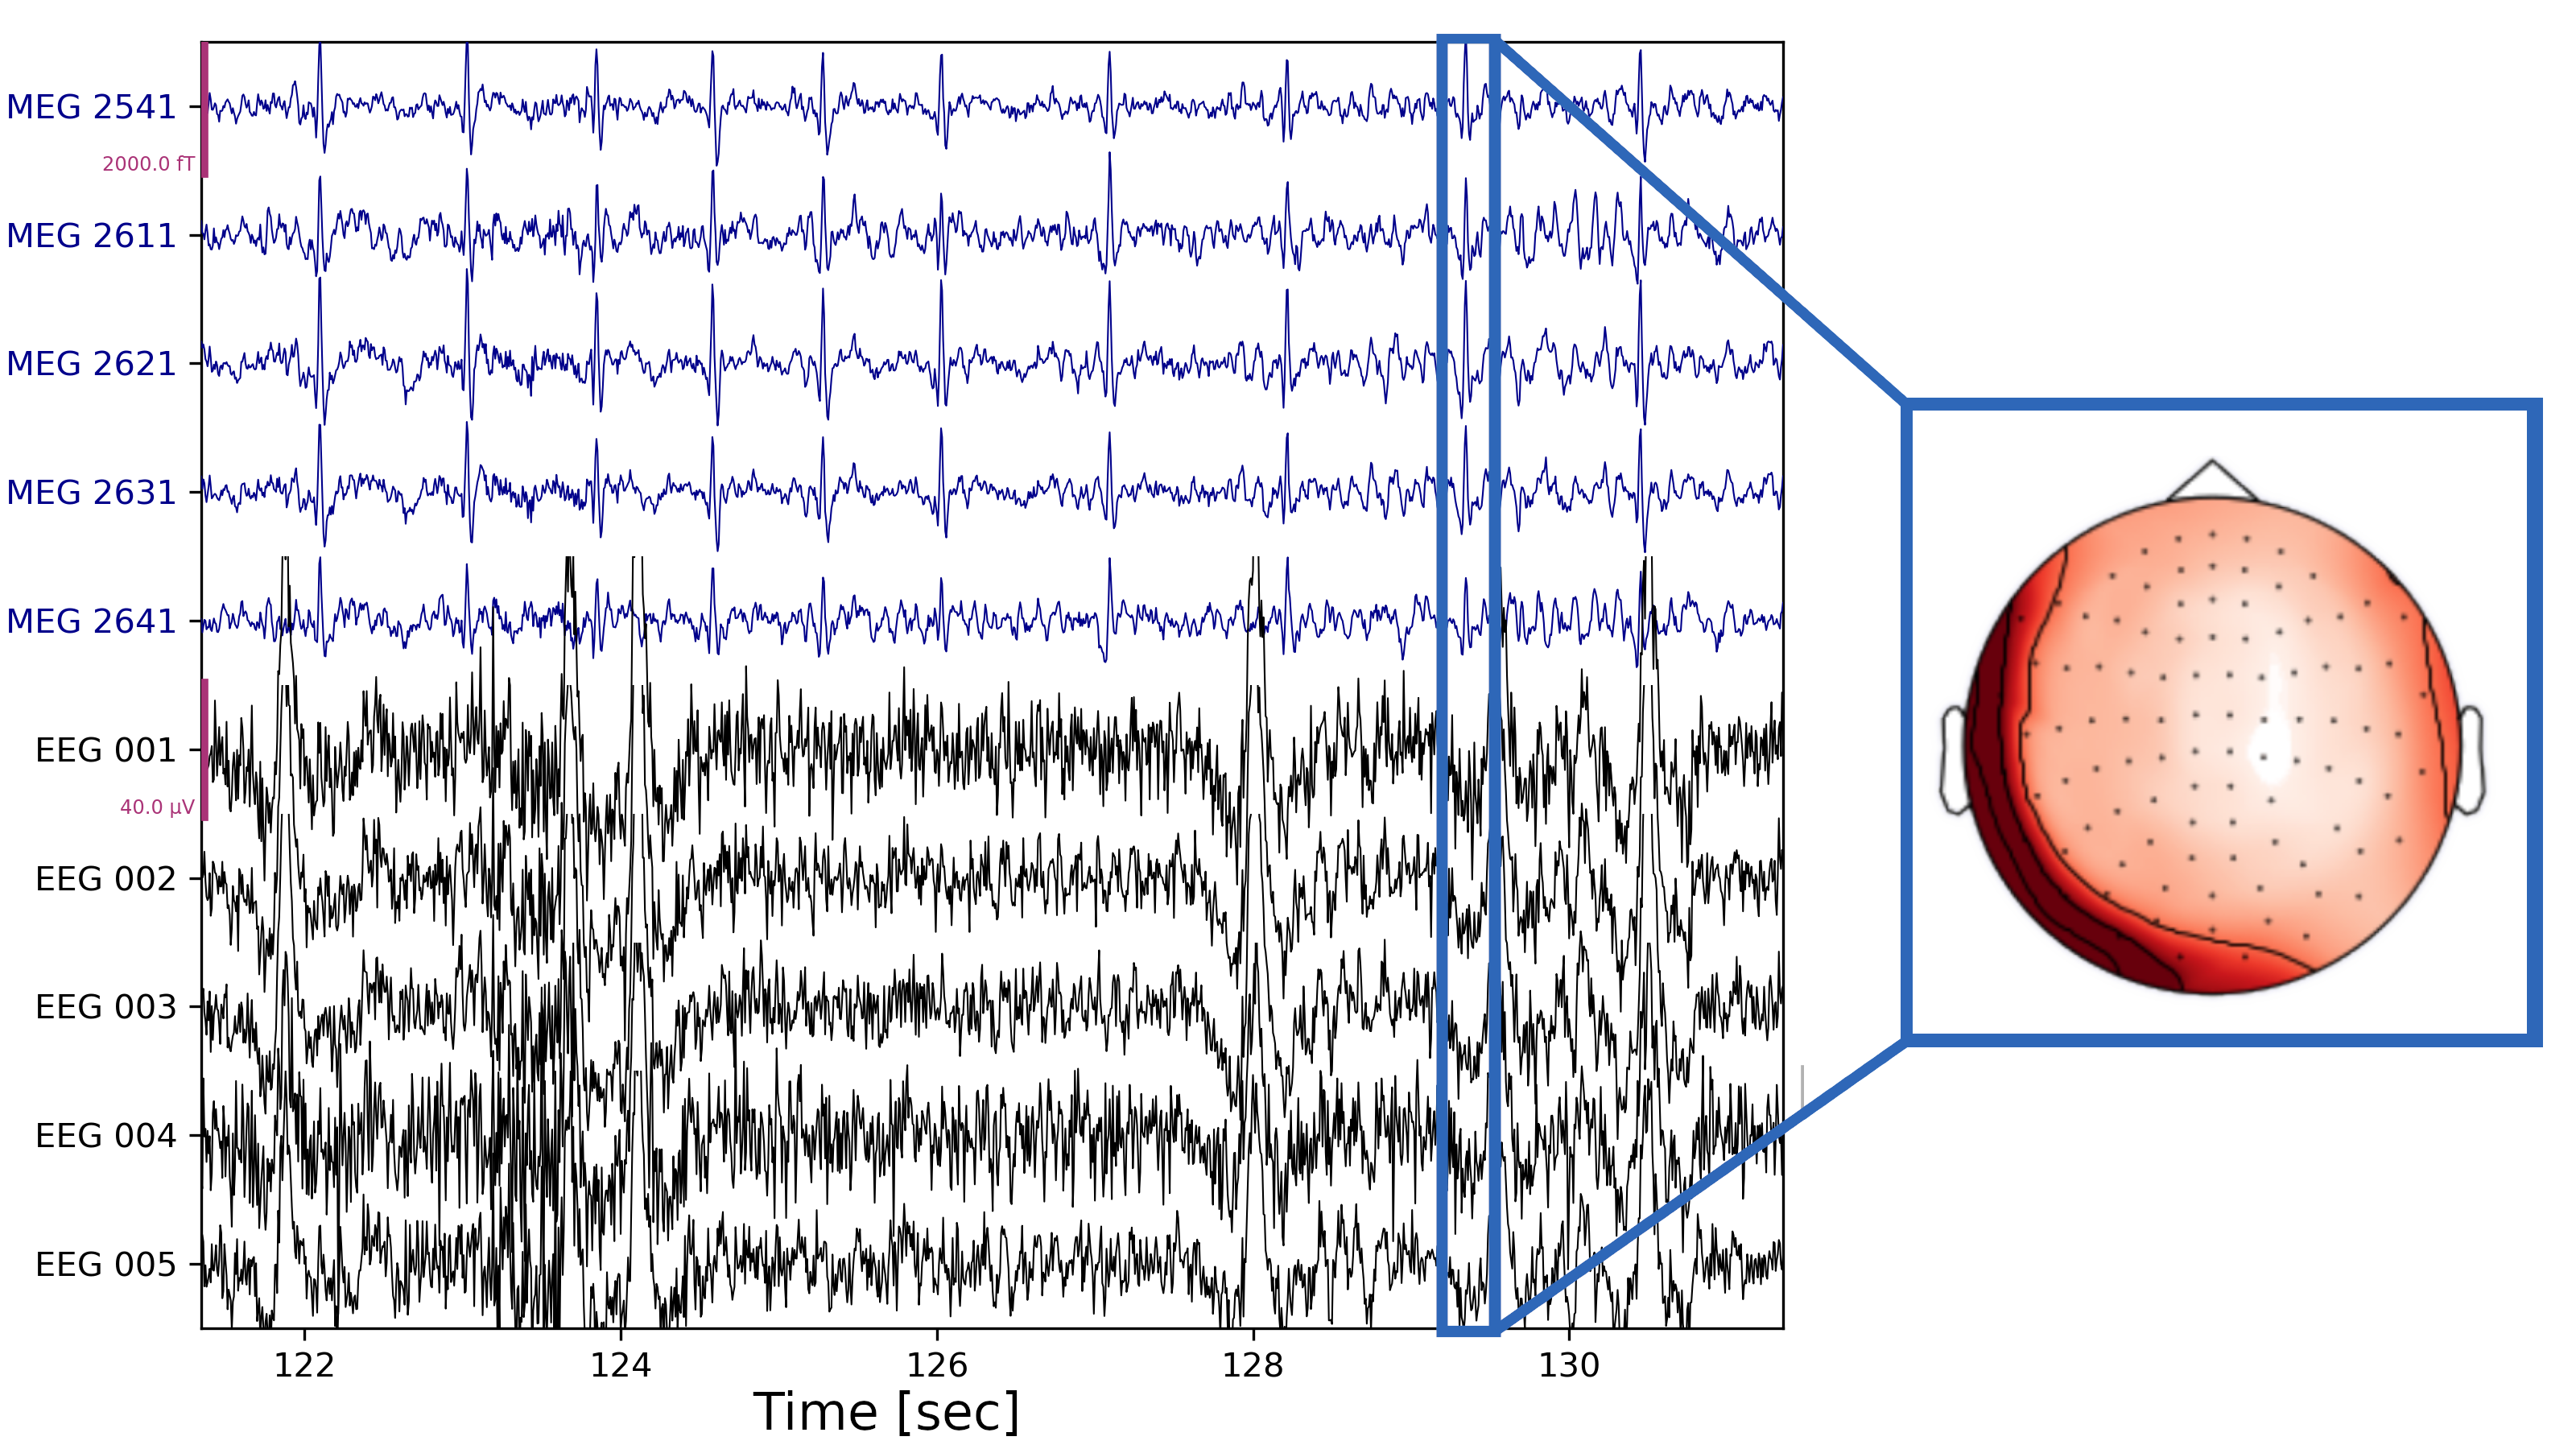
\includegraphics[width=.9\textwidth]{meeg_data_highlight}
    }{
        \alt<1>{
            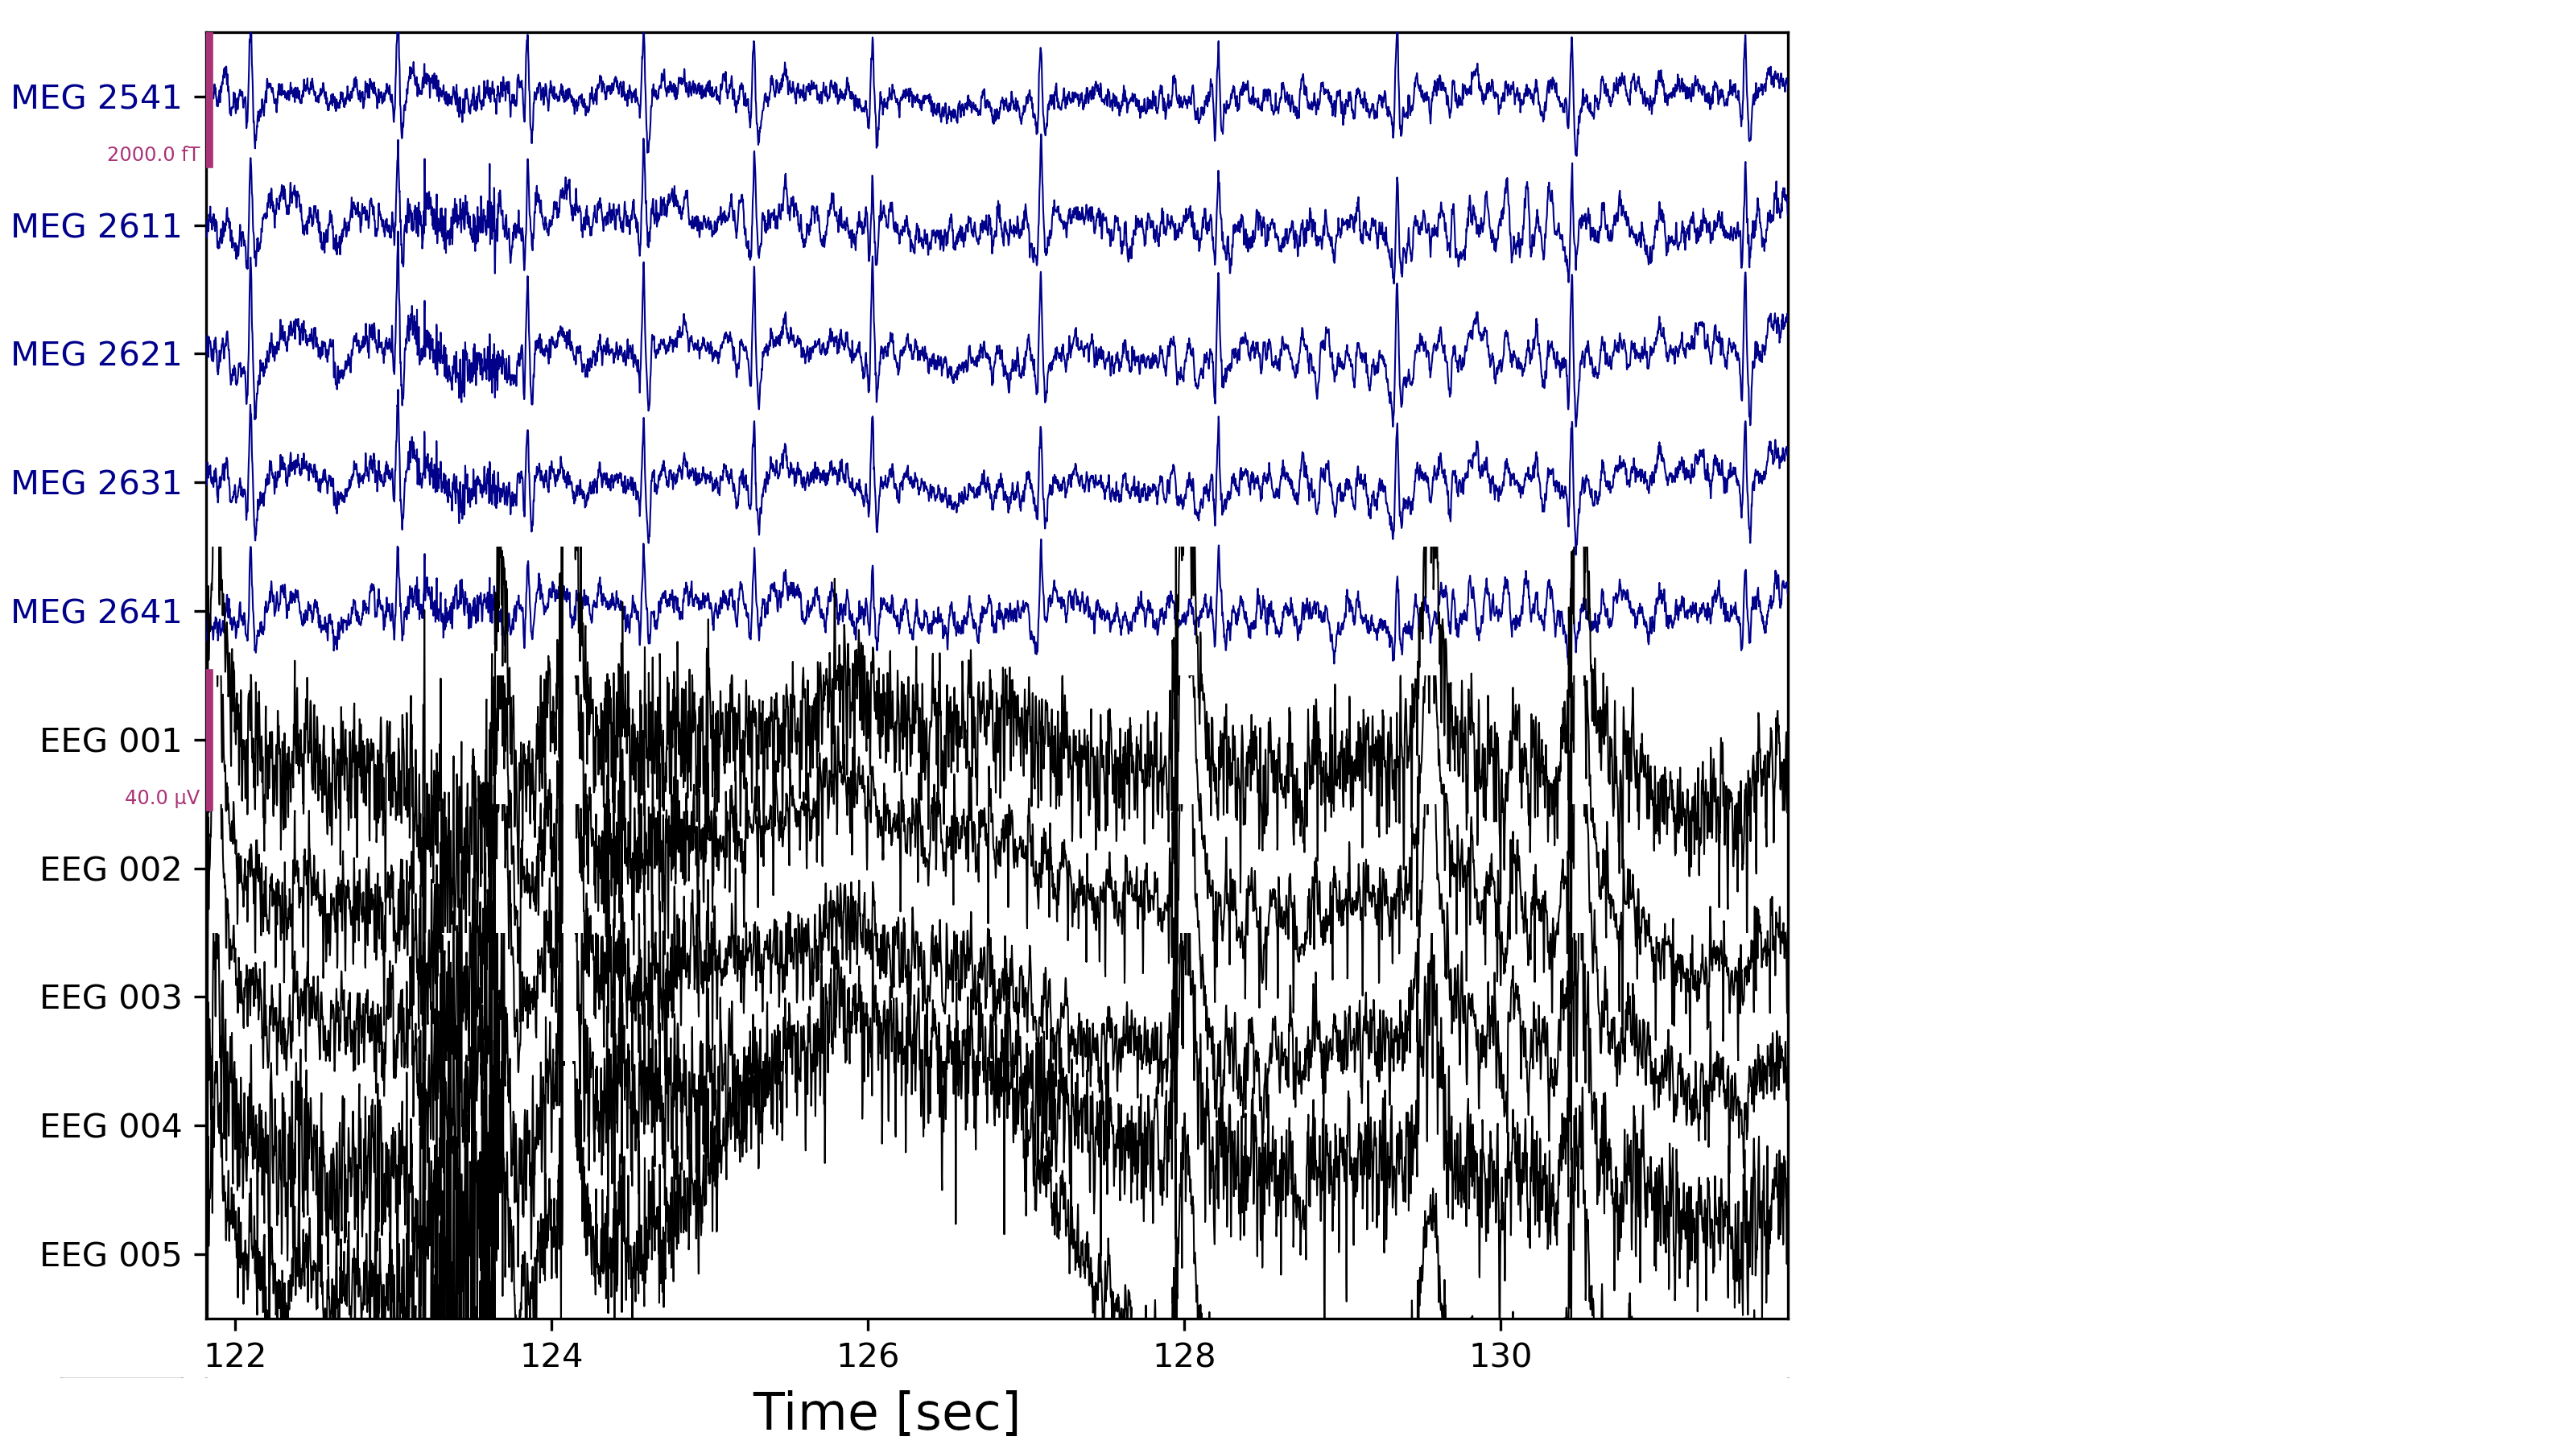
\includegraphics[width=.9\textwidth]{meeg_data}
        }{
            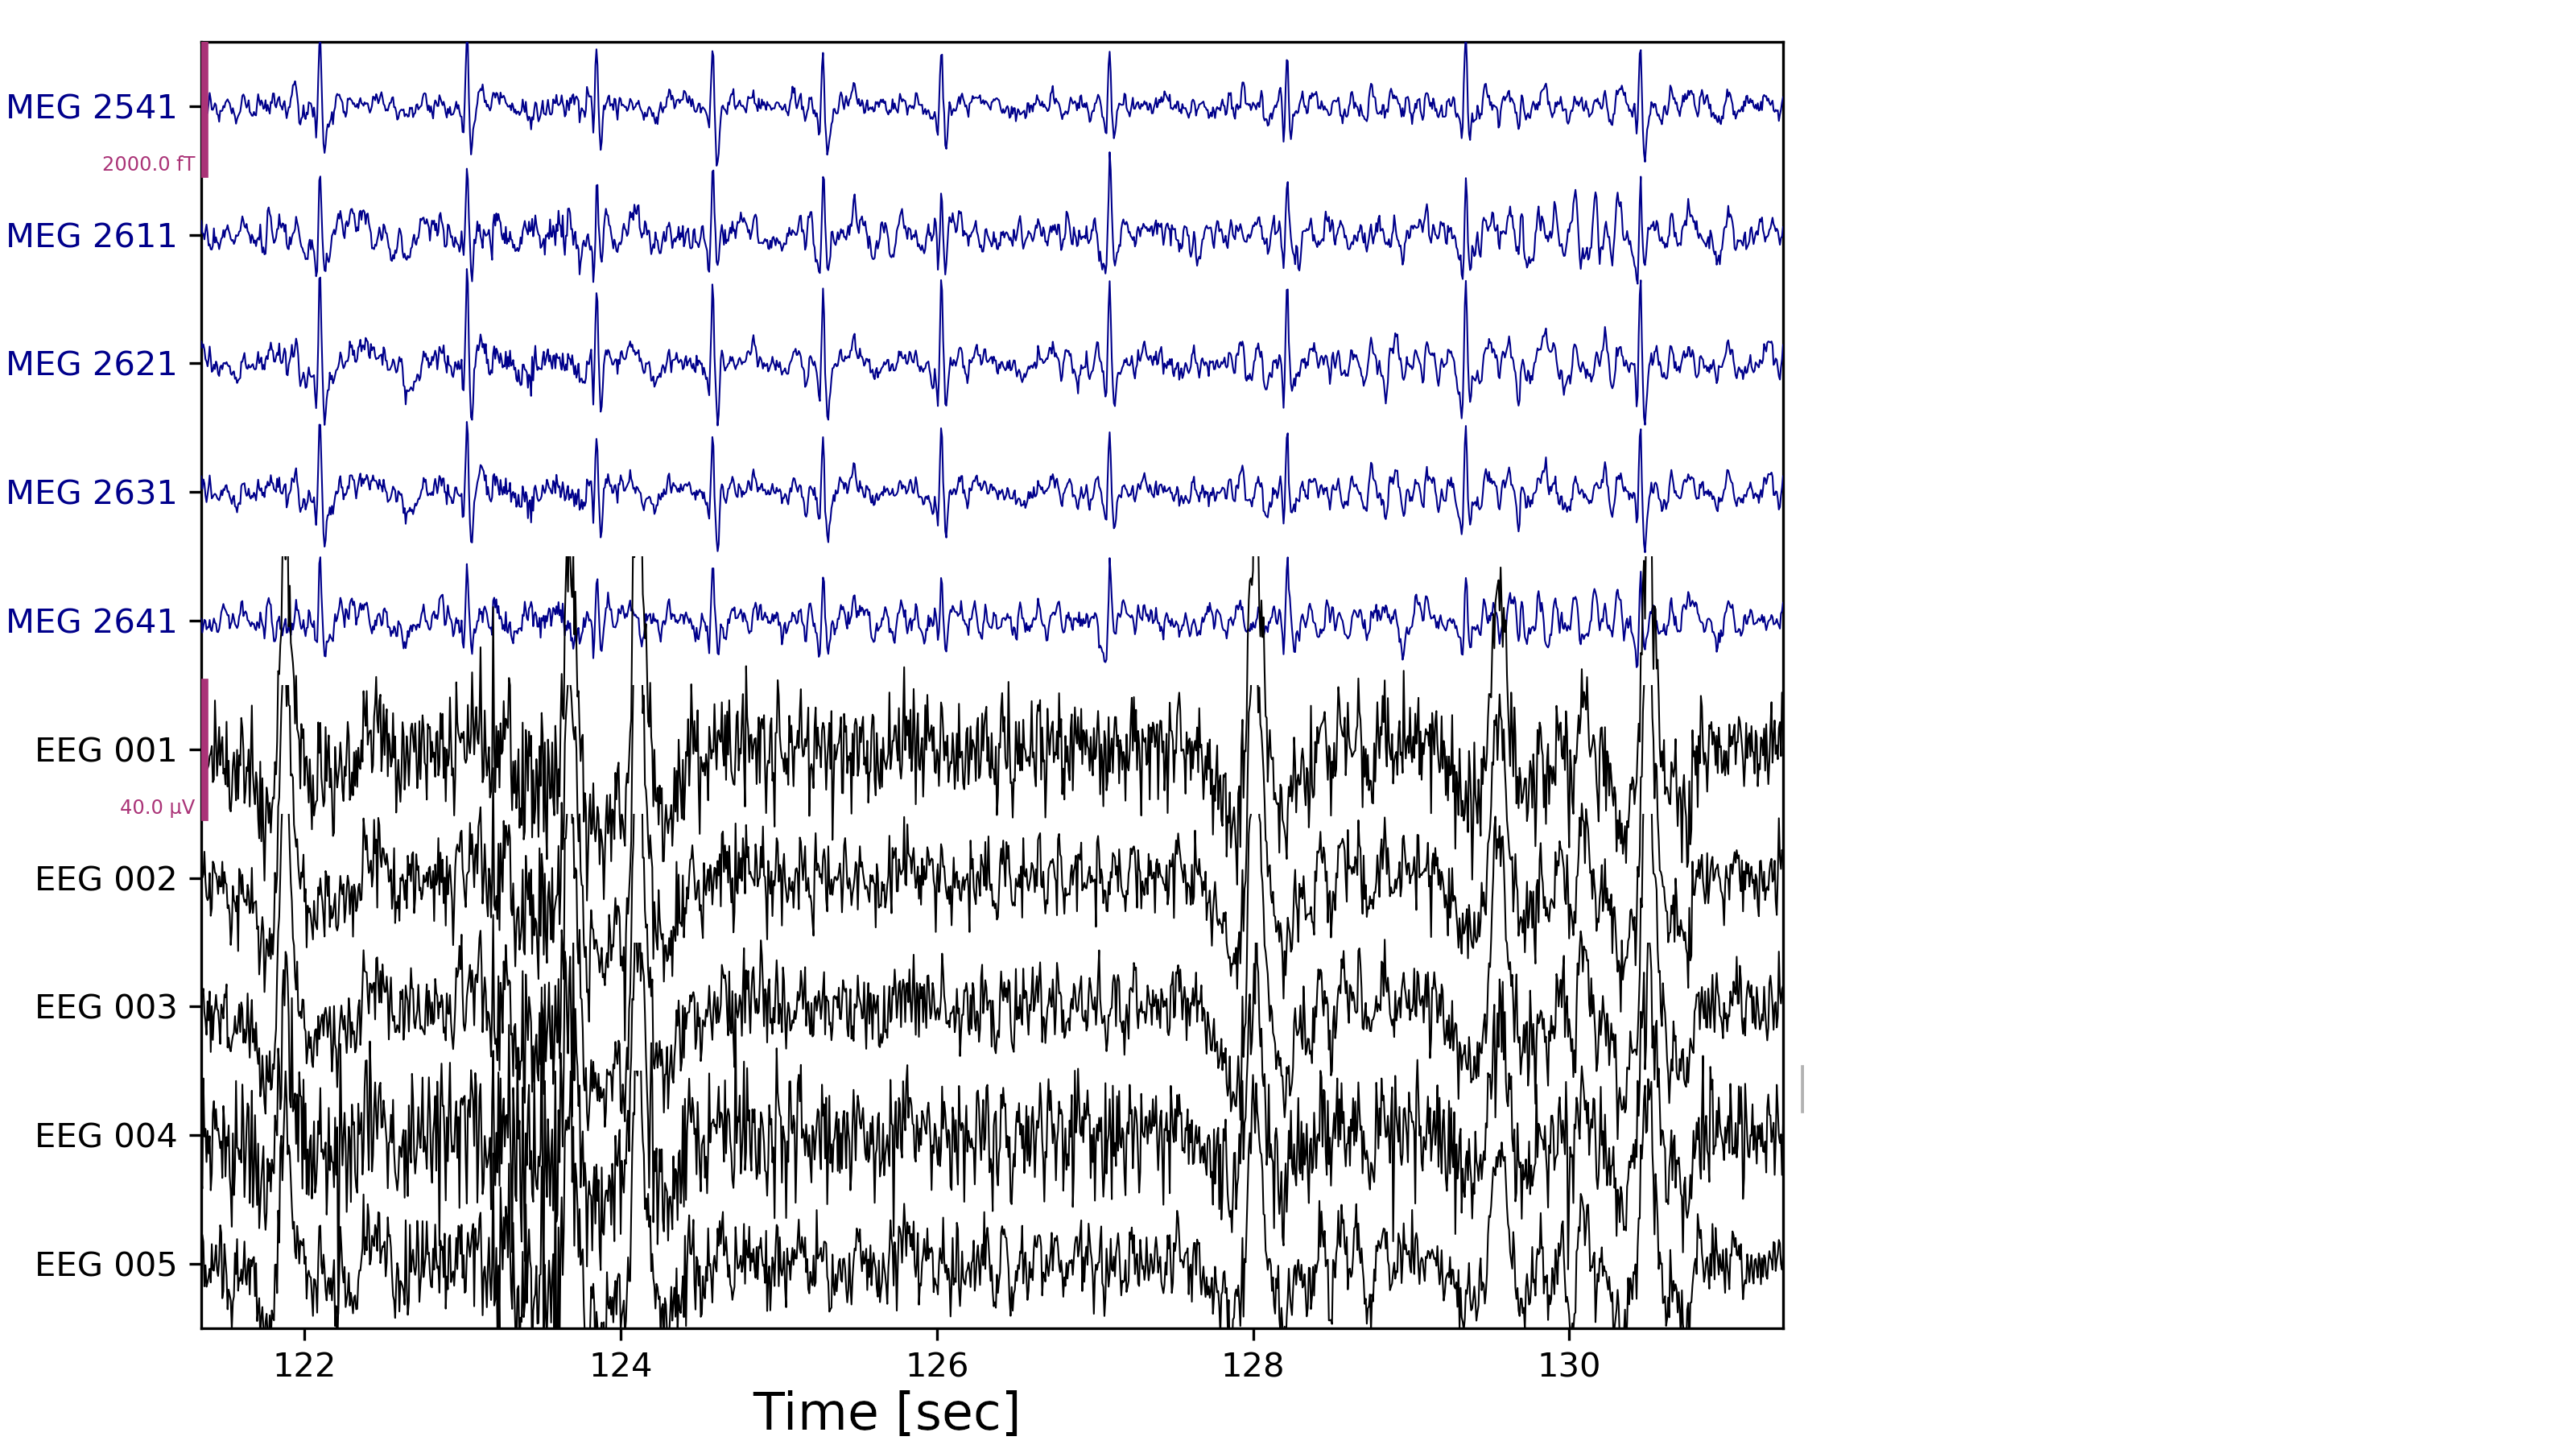
\includegraphics[width=.9\textwidth]{meeg_data_preproc}
        }
    }\\[1em]
    \begin{columns}
        \techterm{Noisy}%
        \techterm{Many artifacts}%
        \techterm{Complex}%
    \end{columns}
}


\frame{
    \frametitle{}

    \begin{columns}[c]
        \column{.6\columnwidth}
    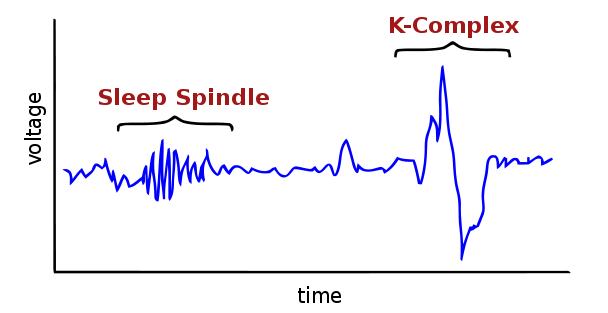
\includegraphics[width=\textwidth, trim={6em 6em 0 0}, clip]{sleep_spinddle}
        \column{.35\columnwidth}
            \highlightbox{
                \centering \Large
                Neural signals exhibit
                diverse and complex
                morphologies
            }
    \end{columns}
    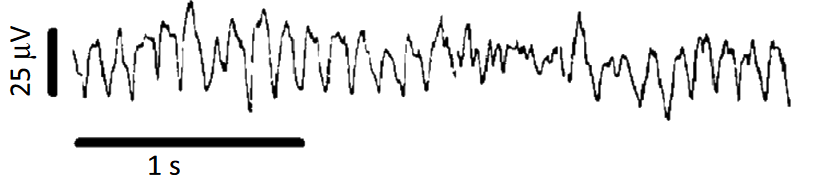
\includegraphics[width=\textwidth]{mu_rythm}\\[-1.5em]
    \rightcite{Cole \& Voytek 2017}
    \vskip-7em
        \begin{columns}[c]
        \column{.75\columnwidth}
        \visible<2->{\highlightbox{\vskip.1em
        \Large Waveform shape can be related to diseases\\
        \eg{} Parkinson \rightcite{Jackson et al. 2019}}\\[.3em]}
        \end{columns}
    \vskip3em
    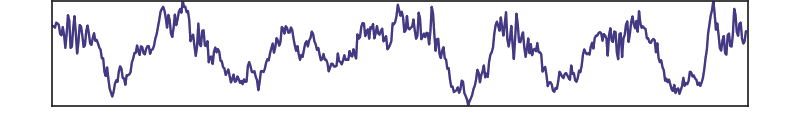
\includegraphics[width=\textwidth]{cfc}\\[-.8em]
    \rightcite{\footnotesize Dupré la Tour et al. 2017}
}

\frame{
    \frametitle{Repeated Stimuli -- Evoked Response \rightcite{Gramfort et al. 2013}}

    \myitem{} Subject is presented some stimuli -- Audio, Visual, Motor, ...\\[.5em]
    \myitem{} Record onset of the stimuli\\[.5em]
    \myitem{} Average signal on window aligned around the stimulus\\[1em]

    \begin{columns}

        \column{.3\textwidth}
        \centering
        Evoked response to an auditory stimuli\\[.5em]
        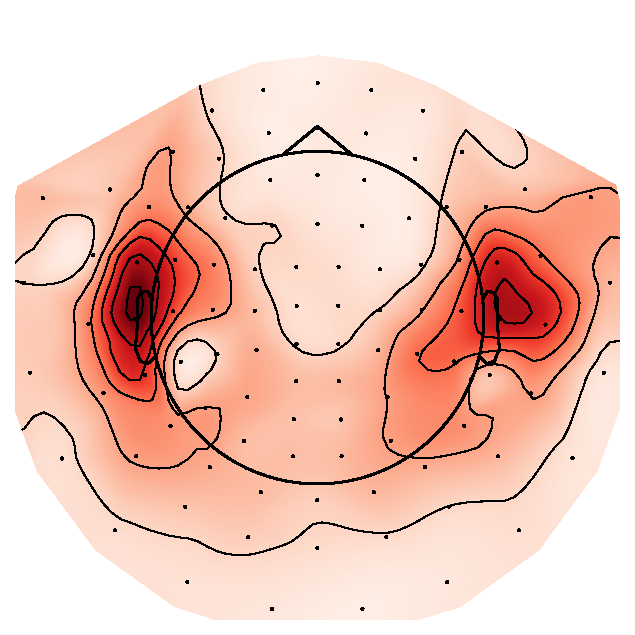
\includegraphics[width=.8\textwidth]{evoked_topo}
        \column{.6\textwidth}
        {\centering
            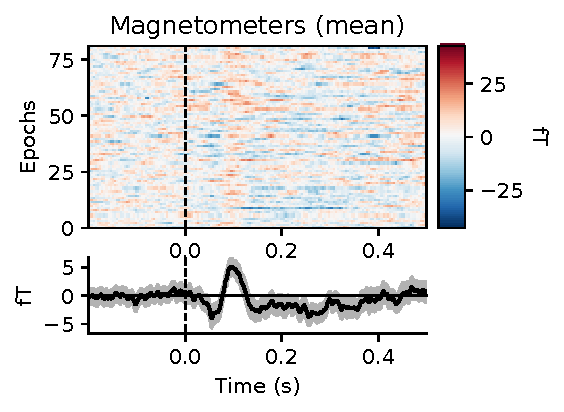
\includegraphics[width=\textwidth]{evoked_response}\\
        }
    \end{columns}
    \rightcite{MNE-Python}
}

\frame{
    \frametitle{Repeated Stimuli -- Induced Response \rightcite{Gramfort et al. 2013}}

    \myitem{} Subject is presented some stimuli -- Audio, Visual, Motor, ...\\[.5em]
    \myitem{} Average PSD on window aligned around the stimulus\\
    \rightcite{MNE-Python}\\[-.5em]

        \centering
        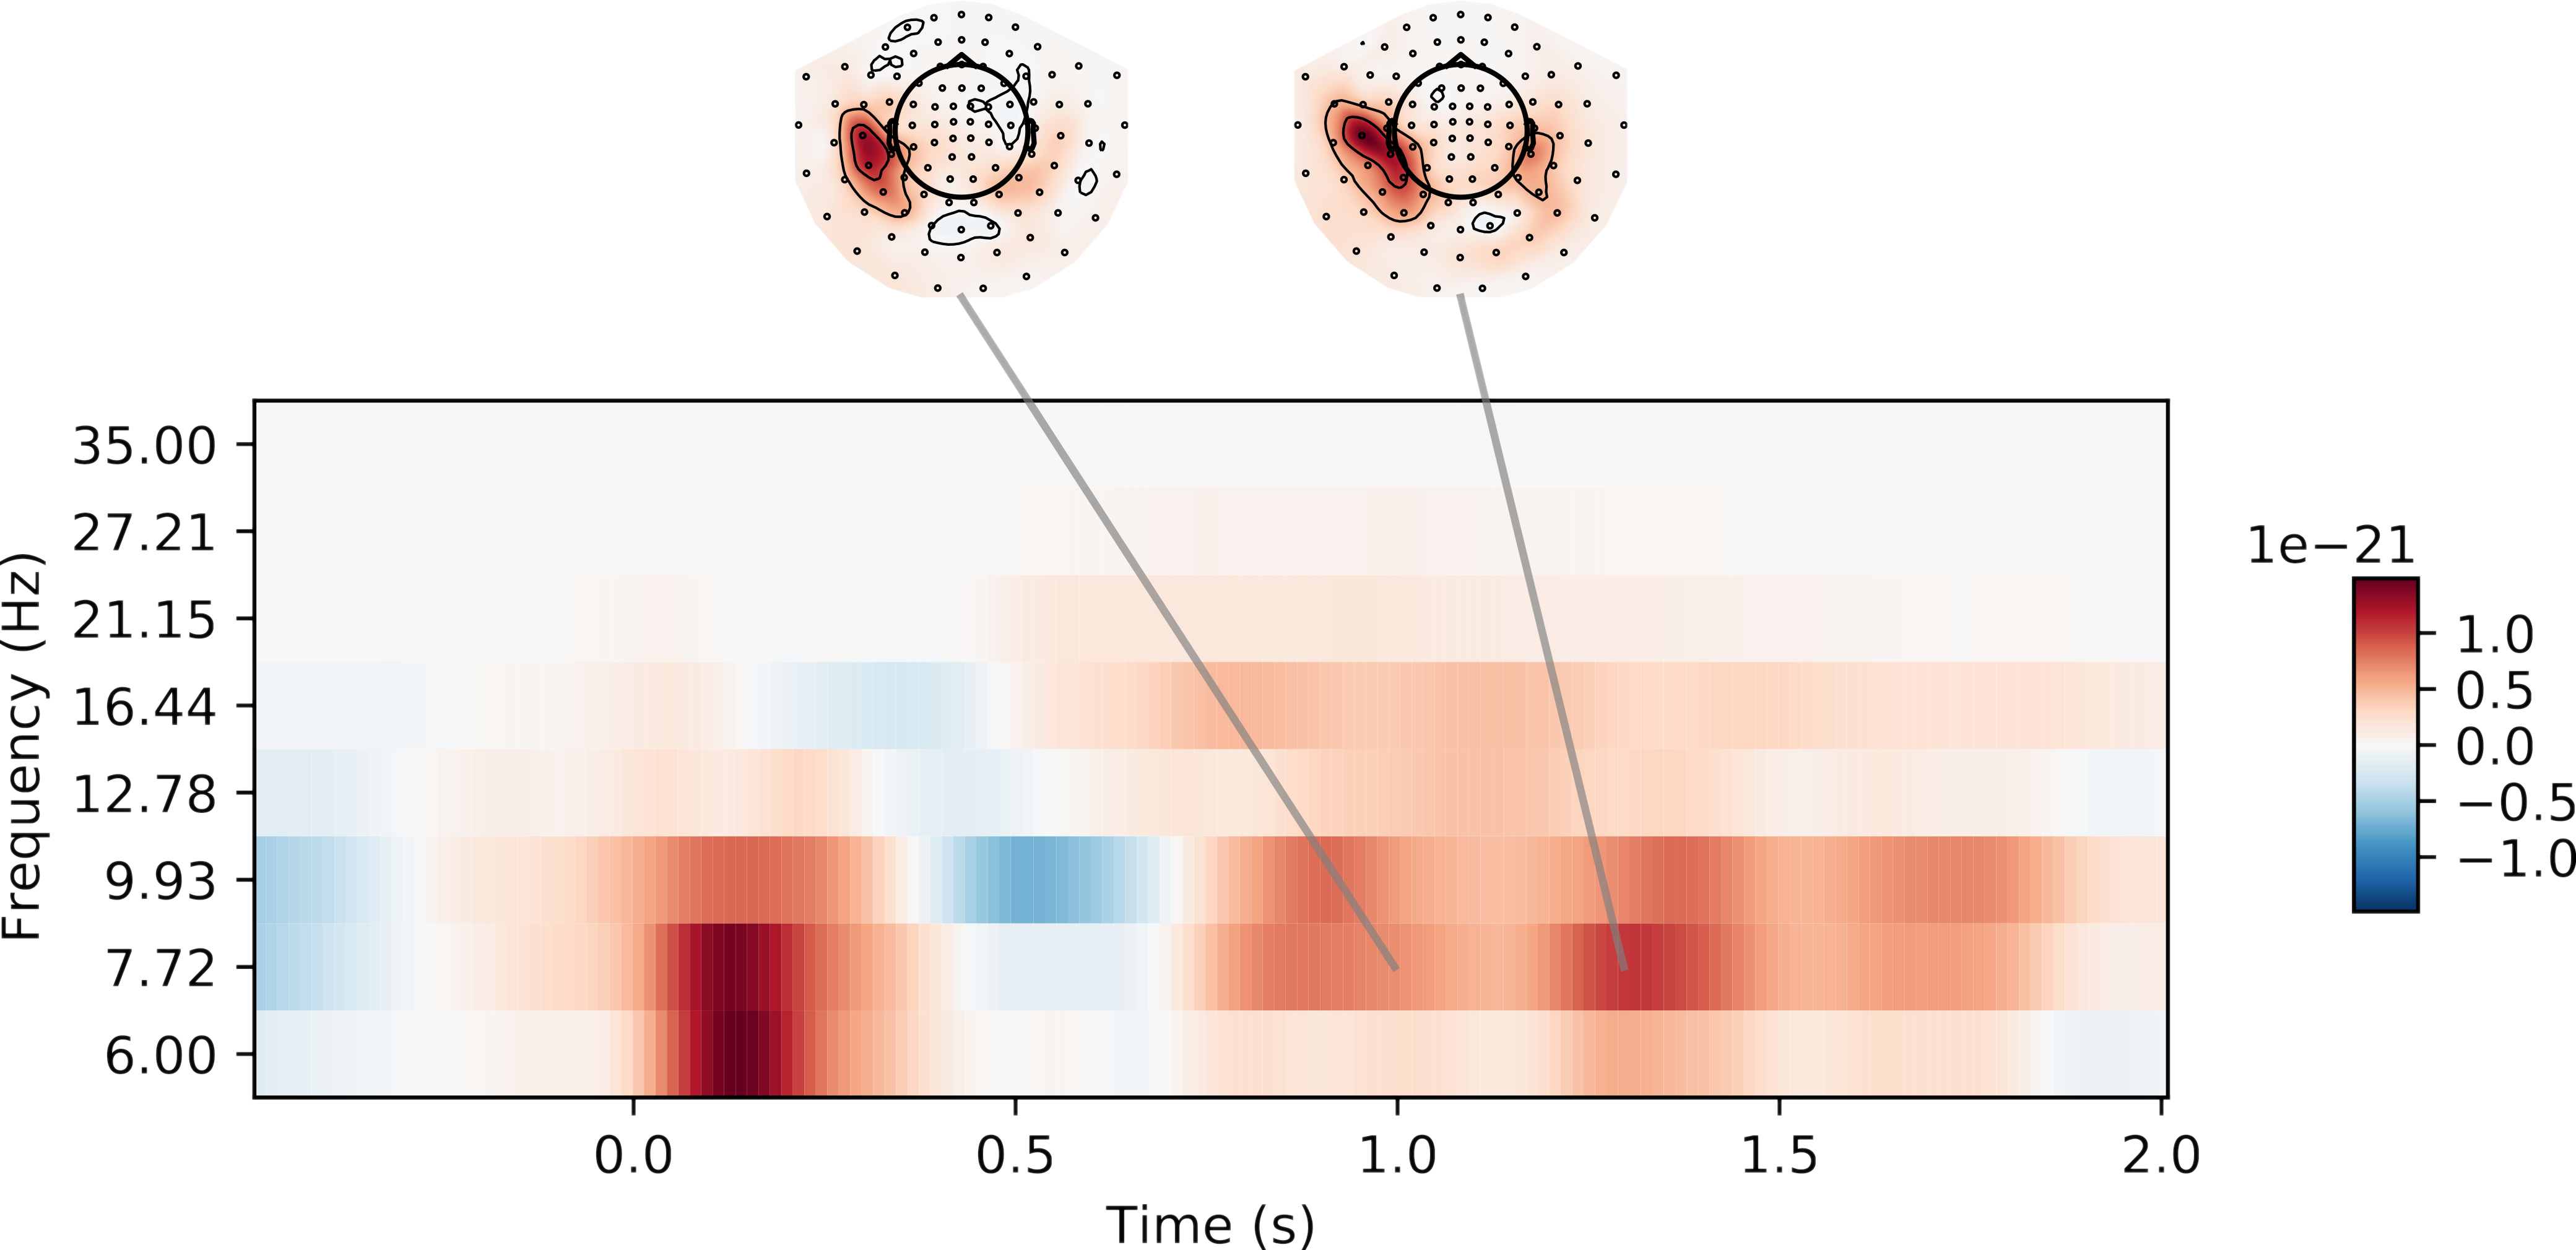
\includegraphics[width=\textwidth]{somato_time_freq.png}\\[.1em]
        Evoked response to an somatosensory stimuli\\

}


\frame{
    \frametitle{How to get back to electrical activity?}

    \definecolor{Z}{RGB}{45,162,65}
    \definecolor{D}{RGB}{180,35,35}
    \def\varX{{\color{linkcolor} \pmb X}}
    \def\varZ{{\color{Z} \pmb \varepsilon}}
    \def\varD{{\color{D} \pmb G}}

    {\centering
    \begin{tikzpicture}
    \tikzset{
        %Define standard arrow tip
        >=stealth',
        %Define style for boxes
        varstyle/.style={
            rectangle,
            rounded corners,
            draw=black,
            text width=1em,
            minimum height=1.5em,
            text centered},
    }
    \node (meg) {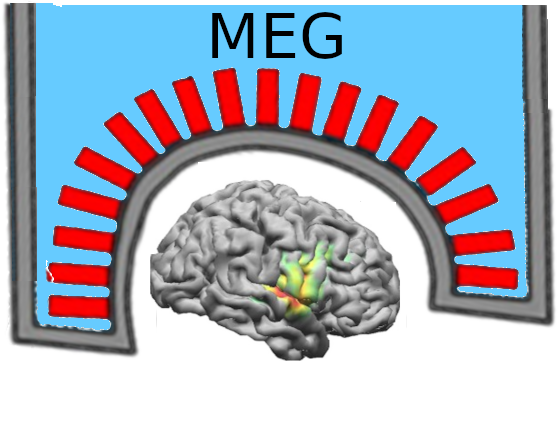
\includegraphics[width=12em]{meg_localised_source}};
    \draw[->, thick] ($(meg.east) - (0, 1.5em)$) -- ++(8em, 0)
    node[midway, align=center] (maxwell) {Maxwell's\\Equations}
    node[right] (topomap) {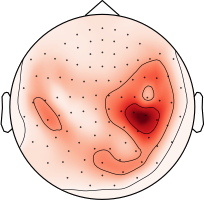
\includegraphics[width=6em]{topomap_somato}};
    \node[varstyle, below=.5em] at (topomap.south) (varX) {$\varX$};
    \node[below=0em of varX.south] {\bf Observed signal};
%        \draw[->, thick] (topomap.east) -- ++(5em, 0)
%        node[midway, align=center] {\small Problème\\ \small inverse}
    \node[varstyle, below=.2em of meg]
        (varZ) {$\varZ$};
    \node[below=0em of varZ.south] {\bf Electrical activity};
    \node[varstyle, below=3.8em of maxwell.center]
        (varD) {$\varD$};

    \uncover<2->{
         \draw[<-, thick] (meg.east) to[bend left, looseness=1]
            node [midway, above] {Inverse Problem}
            ($(topomap.west) + (0, 1.5em)$);
    }
    \end{tikzpicture}}
    \vskip0em
    {\bf Forward model: }$\varX{} = \varD\varZ$
    \hskip3em
    \uncover<2->{{\bf Inverse problem:} $\varZ = f(\varX)$ (ill-posed)}\\[1em]
    \uncover<3->{\centering
        \myitem{} Dipole fit
        \hskip2em
        \myitem{} Regularized optimization
        \hskip2em
        \myitem{} Deep-learning\\
        \mycite{Sarvas1987}\hskip2em
        \mycite{Gramfort2012}\hskip2em
        \mycite{Hecker2021}
    }

}


\section{Learning the waveform:\\Convolutional Dictionary Learning}
\parttitleframe{Grosse2007}

\frame[t]{
	\frametitle{Local structure in signals}

	\visible<5->{
		\textbf{Key idea}: decouple the localization of the
							patterns and their shape}
    \vskip.5em%
    \centering%
    \only<1>{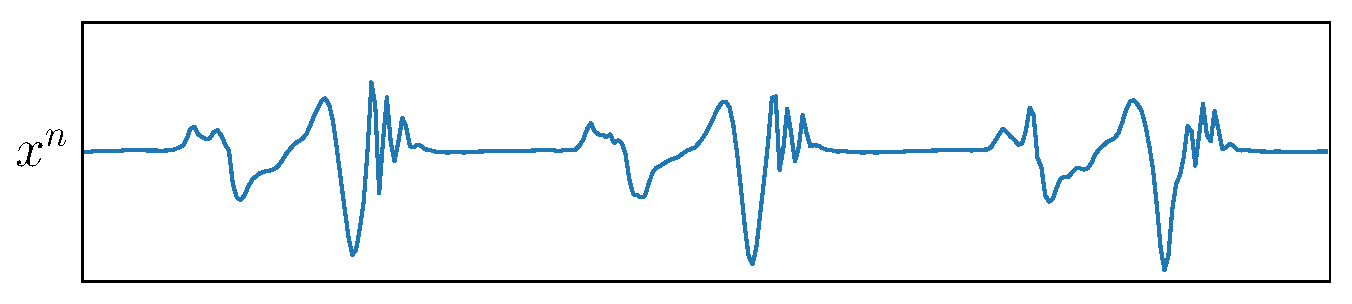
\includegraphics[width=\textwidth]{intro_csc_0}}%
    \only<2>{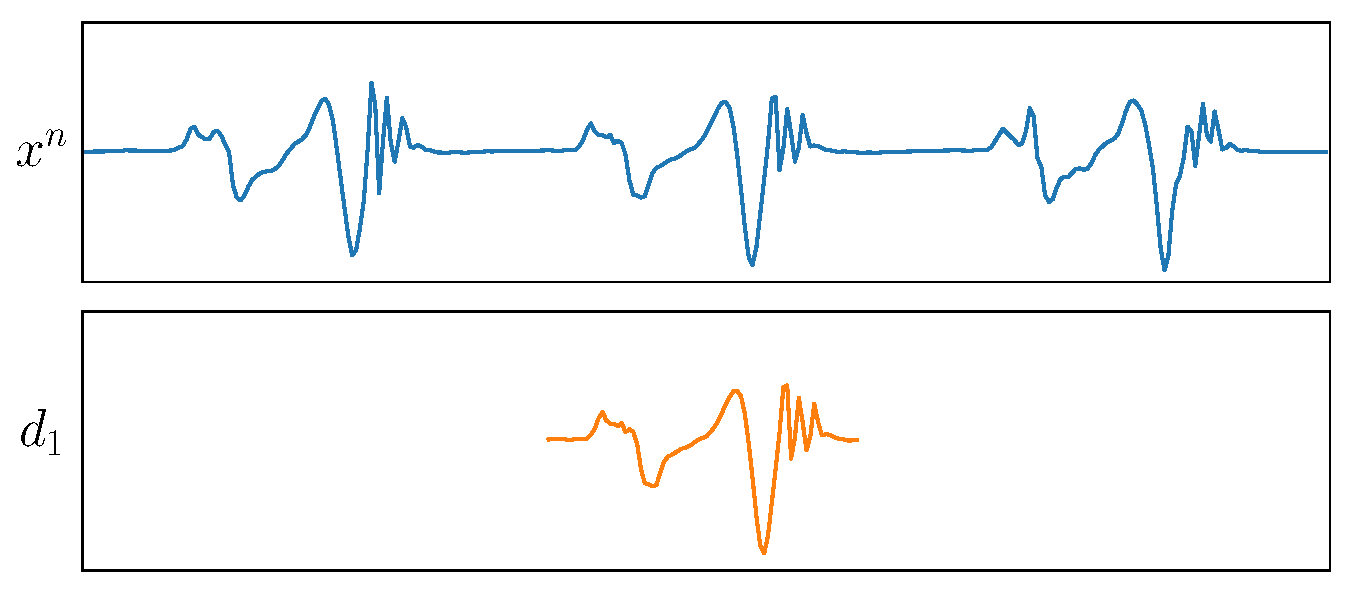
\includegraphics[width=\textwidth]{intro_csc_1}}%
    \only<3>{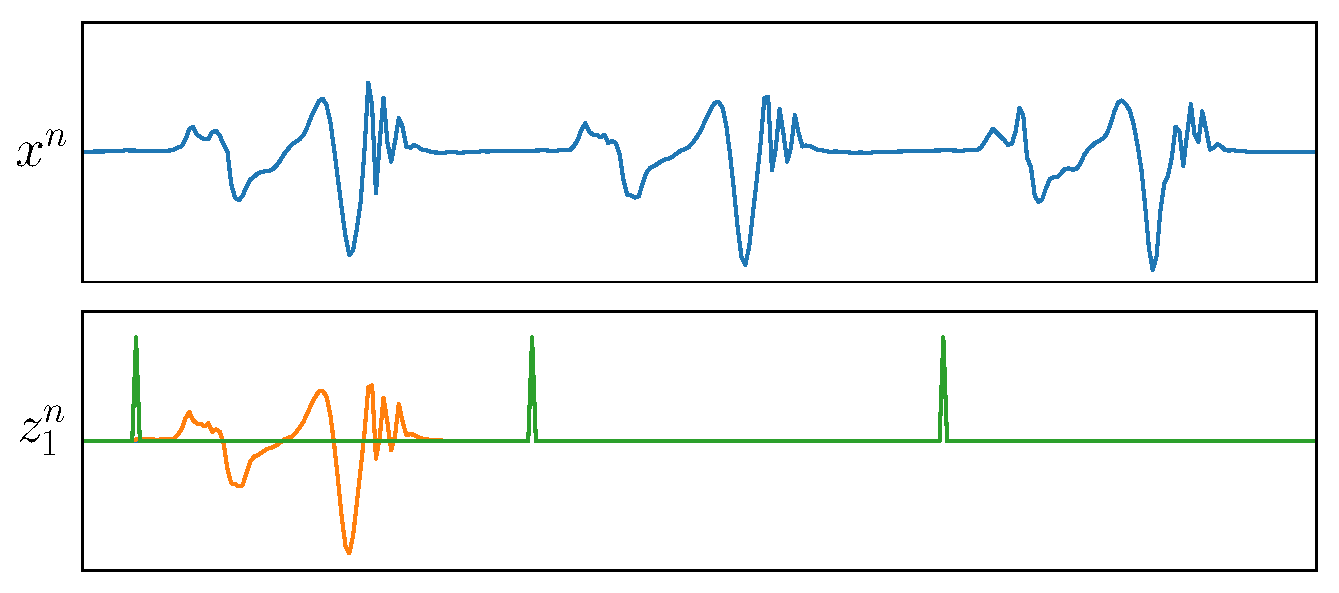
\includegraphics[width=\textwidth]{intro_csc_2}}%
    \only<4>{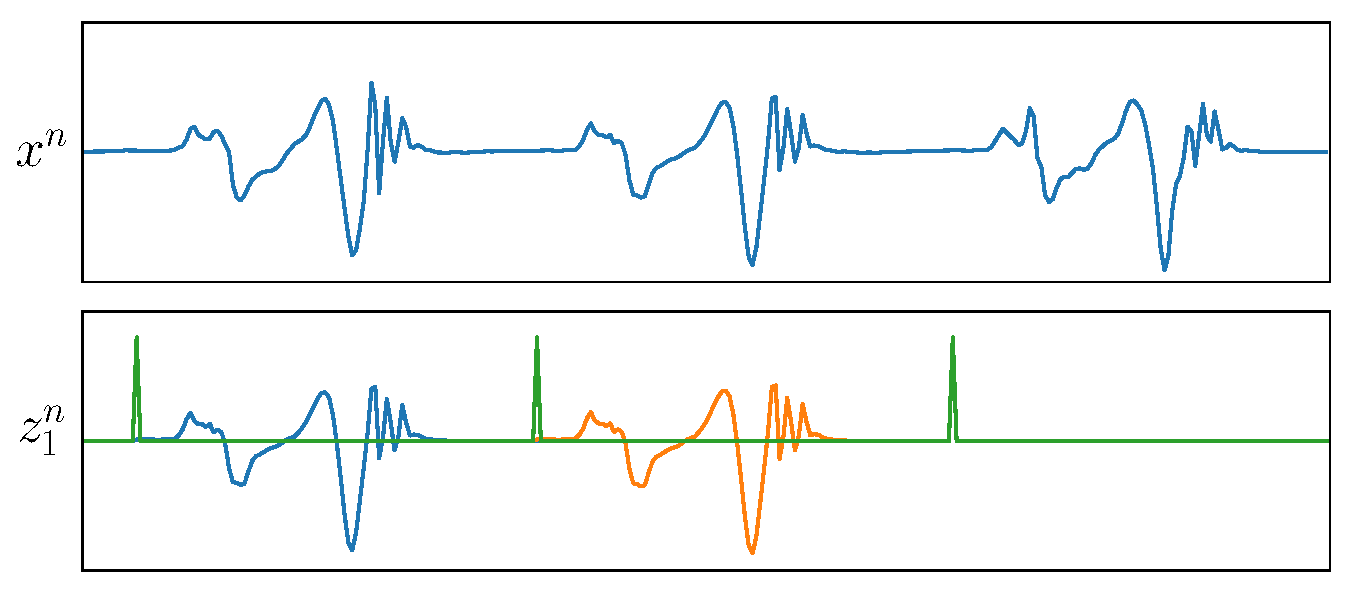
\includegraphics[width=\textwidth]{intro_csc_3}}%
    \only<5>{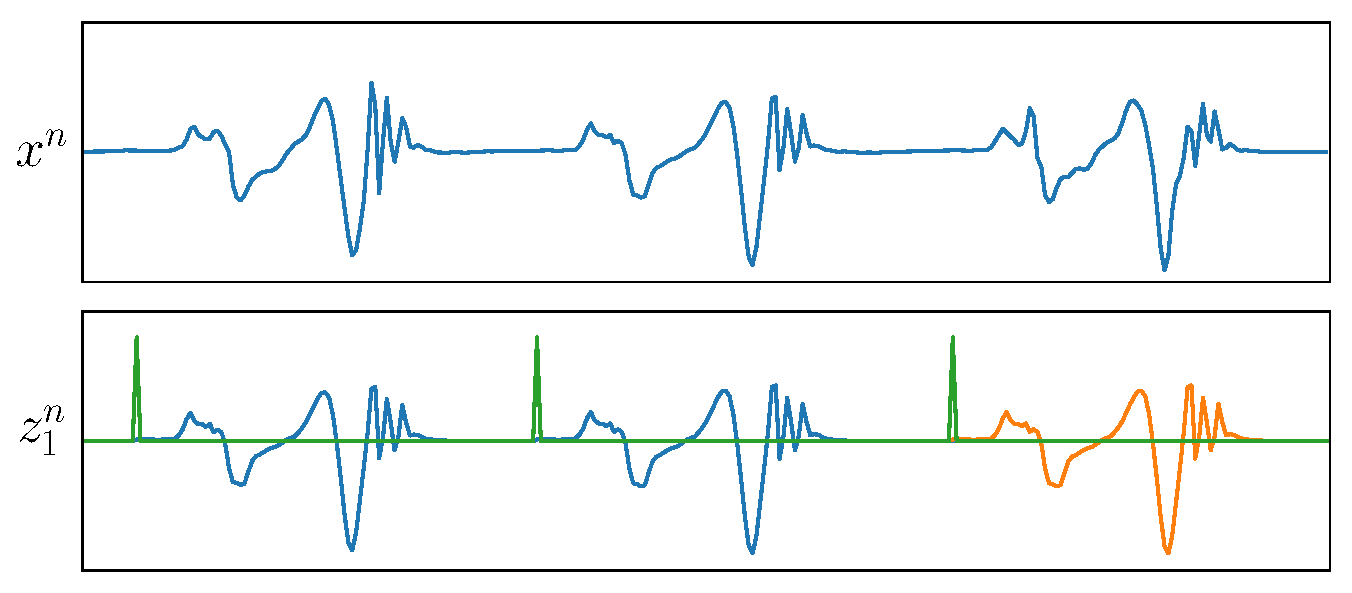
\includegraphics[width=\textwidth]{intro_csc_4}}%
    \only<6->{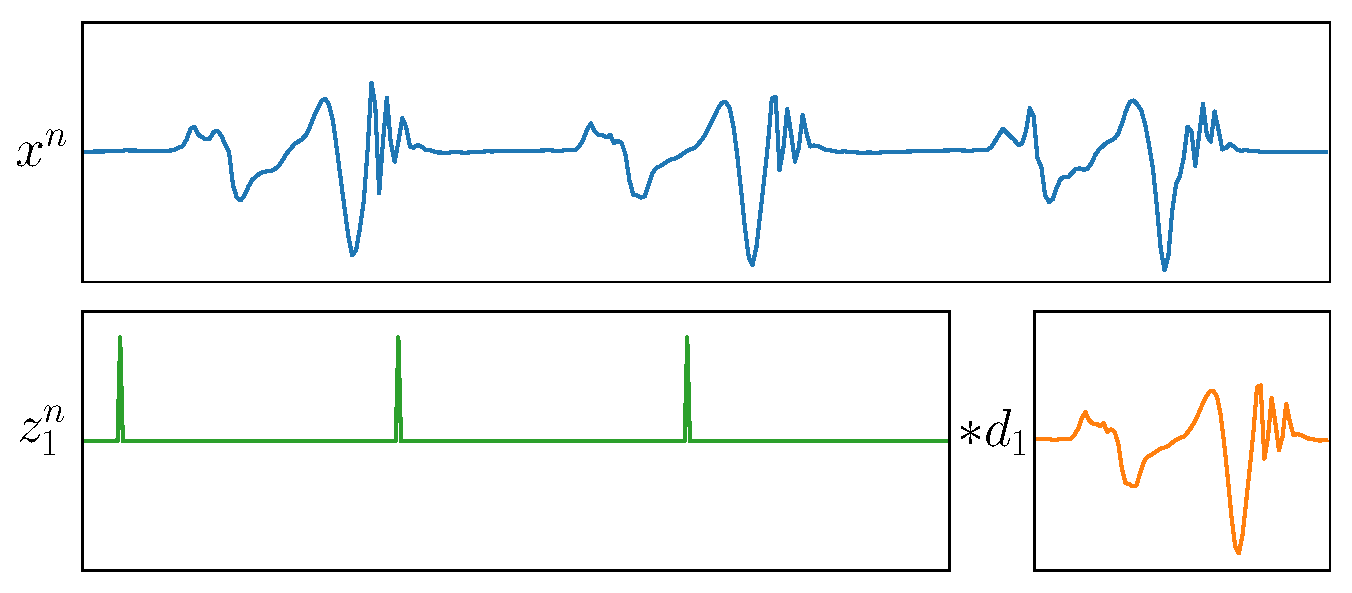
\includegraphics[width=\textwidth]{intro_csc_5}}%
    \vskip0em%
    \only<7>{%
        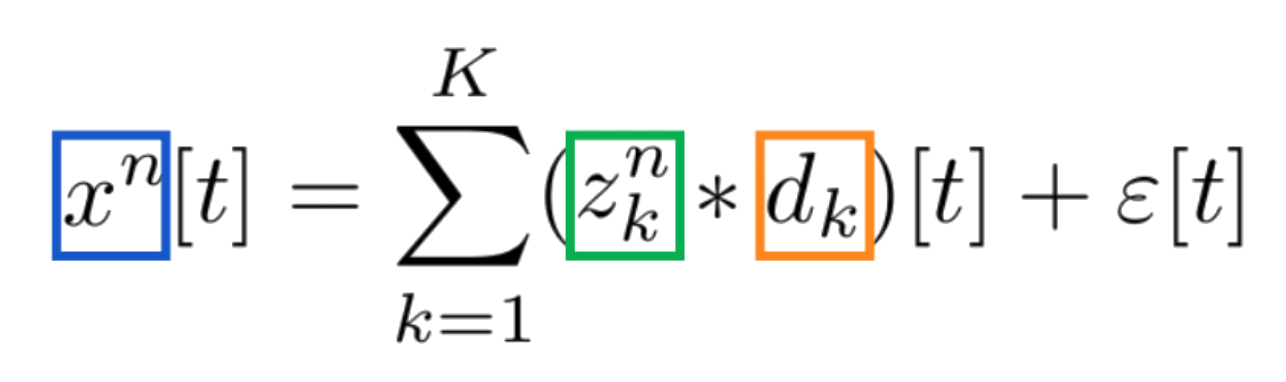
\includegraphics[width=.6\textwidth]{csc_explain_eq_color}%
    }
}

\frame{
    \frametitle{Convolutional Dictionary Learning \mycite{Grosse2007}}

    For a set of $N$ univariate signals $x^n$, solve\\[.5em]
        {\centering 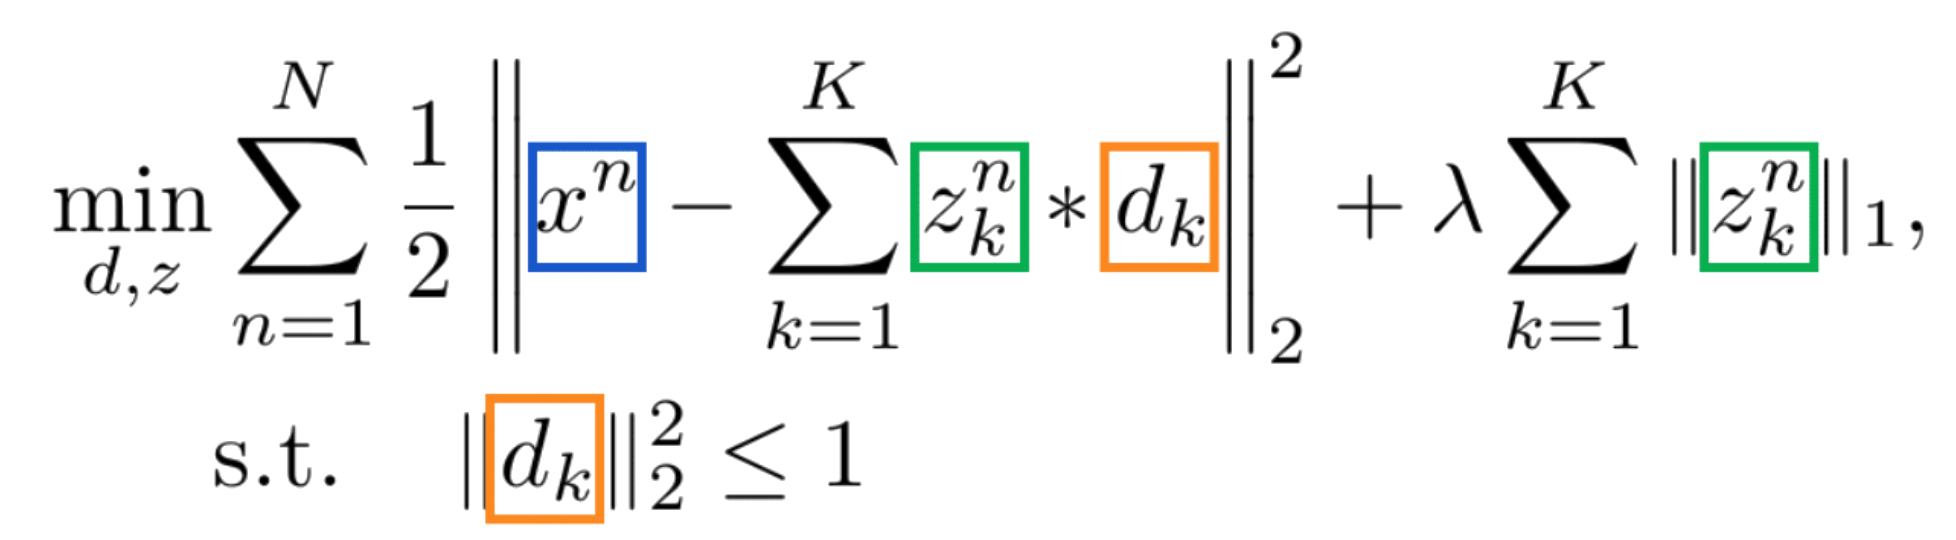
\includegraphics[width=.8\textwidth]{csc_eq_l1}\\[1em]}
    \textbf{Hypothesis:} patterns $d_k$ are not present everywhere in the signal. They are localized in time.
    \strongpoint{Sparse activation signals $z$}
    \vskip2em
    \textbf{Technical hypothesis:} the patterns are in the $\ell_2$-ball: $\|d_k\|_2^2 \le 1$.
}

% \frame{
%     \frametitle{Optimization strategy}
%     \textbf{Bi-convex:} The problem is not jointly convex in $z^n_k$, and  $d_k$
%     but it is convex in each block of coordinate.\\[1em]

%     \textbf{Alternate minimization} (\emph{a.k.a.} Bloc Coordinate Descent):\\[.5em]

%     \begin{itemize}\itemsep.5em
%     \item \textbf{Z-step:} given a fixed estimate of the atom, compute the activation signal $z^n_k$ associated to each signal $x^n$.
%     \item \textbf{D-step:} given a fixed estimate of the activation, update the atoms in the dictionary $d_k$.
%     \end{itemize}

%     \vskip1em
%     \textbf{Unrolled optimization}:\\[.5em]

%     \begin{itemize}\itemsep.5em
%     \item \textbf{Z-step:} use an fixed differentiable procedure $f(x^n, D)$.
%     \item \textbf{D-step:} learn $D$ through back-propagation.
%     \end{itemize}
%     \rightcite{Malezieux et al. 2022}
% }

% \begin{frame}{How to extend CSC to multivariate signals?}
%     We can just use multivariate convolution,
%     \[
%         \underbrace{X[t]}_{\in\Rset^P} = \sum_{k=1}^K \left(z_k * D_k\right)[t] = \sum_{k=1}^K \sum_{\tau=1}^L z_k[t-\tau] \underbrace{D_k[\tau]}_{\in \Rset^P}
%     \]
%     with:
%     \begin{itemize}
%         \item $X$ a multivariate signal of length $T$ in $\Rset^P$
%         \item $D_k$ a multivariate signal of length $L$ in $\Rset^P$
%         \item $z_k$ a univariate activation signal of length $\widetilde{T} = T - L + 1$
%     \end{itemize}
%     \vskip1em
%     However, this model does not account for the physics of the problem.
% \end{frame}


\section{Rank-1 constrained dictionary learning}
\parttitleframe{DuprelaTour2018}


\begin{frame}{EM wave diffusion}
	\begin{itemize}
		\uncover<1->{\item Recording here with 8 sensors}
		\uncover<2->{\item EM activity in the brain}
		\uncover<3->{\item The electric field is spread \textbf{linearly} and \textbf{instantaneously} over all sensors (Maxwell equations)}
	\end{itemize}
	\centering
	\only<1>{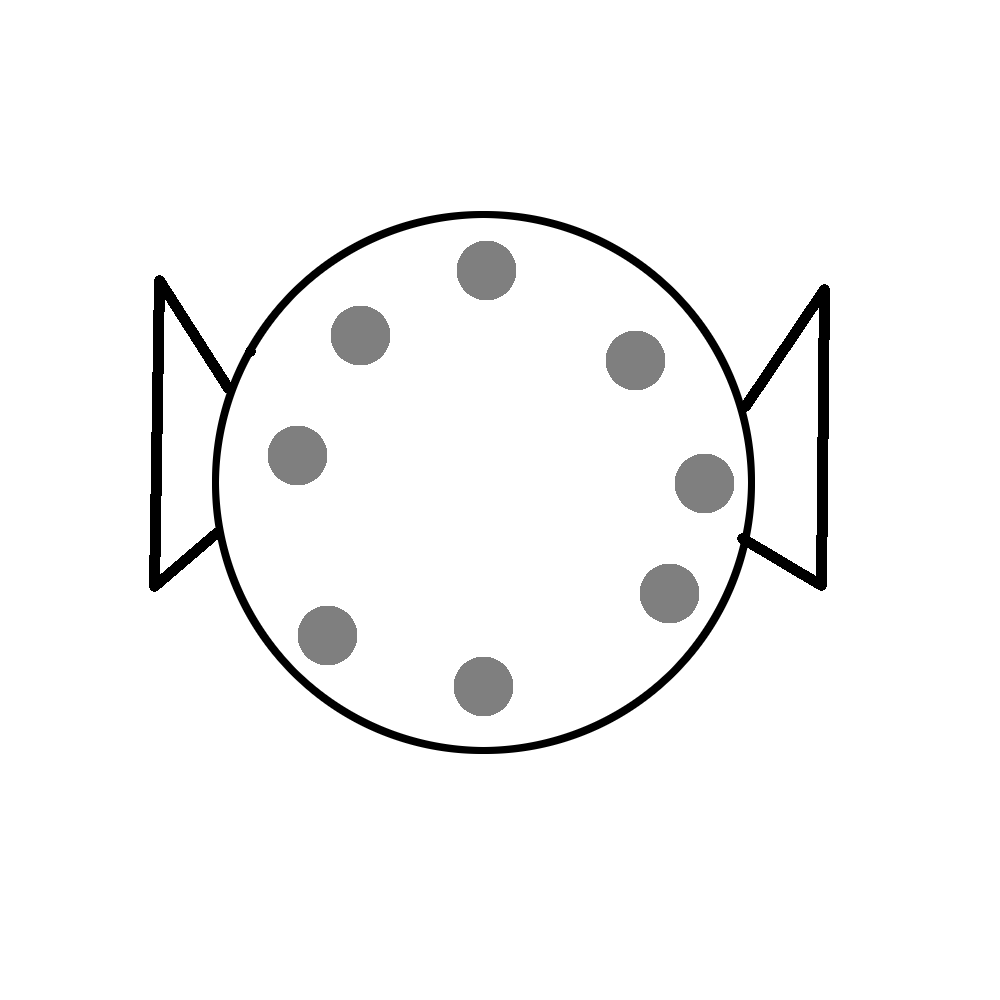
\includegraphics[width=.5\textwidth]{physic1}}%
	\only<2>{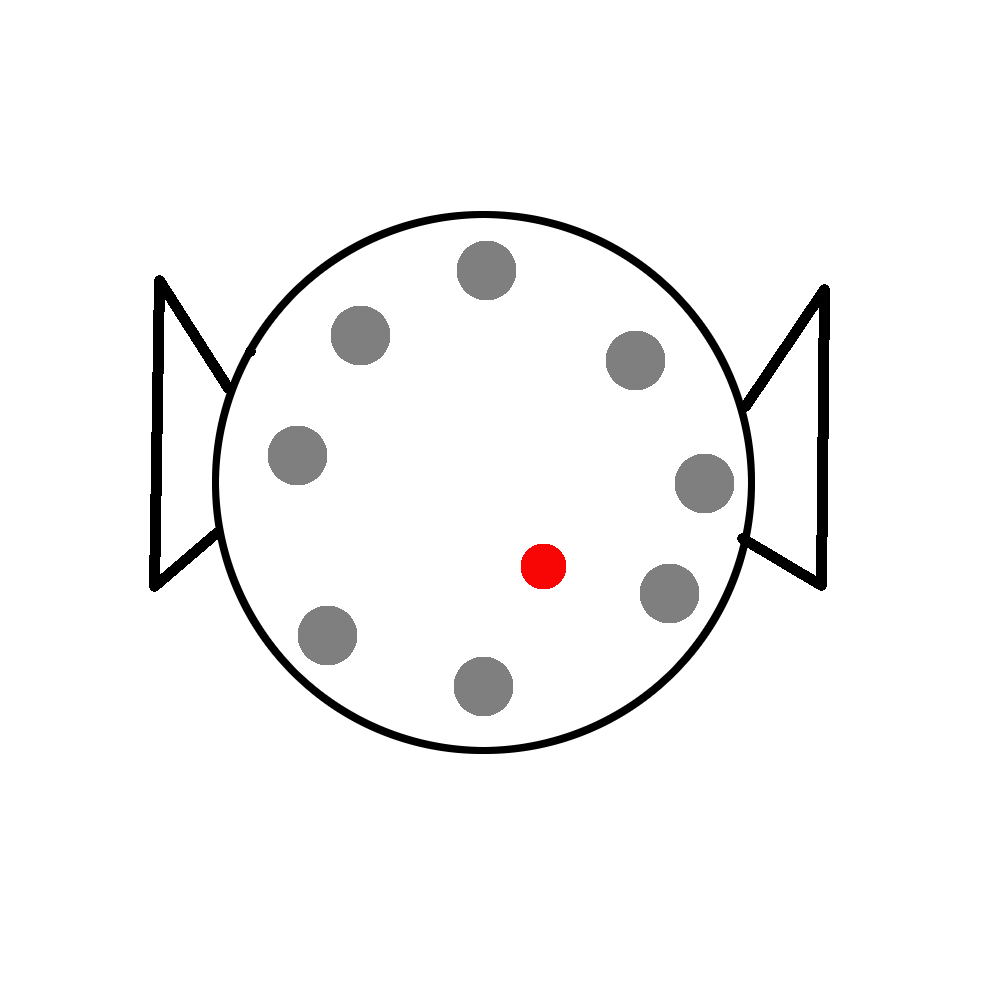
\includegraphics[width=.5\textwidth]{physic2}}%
	\only<3>{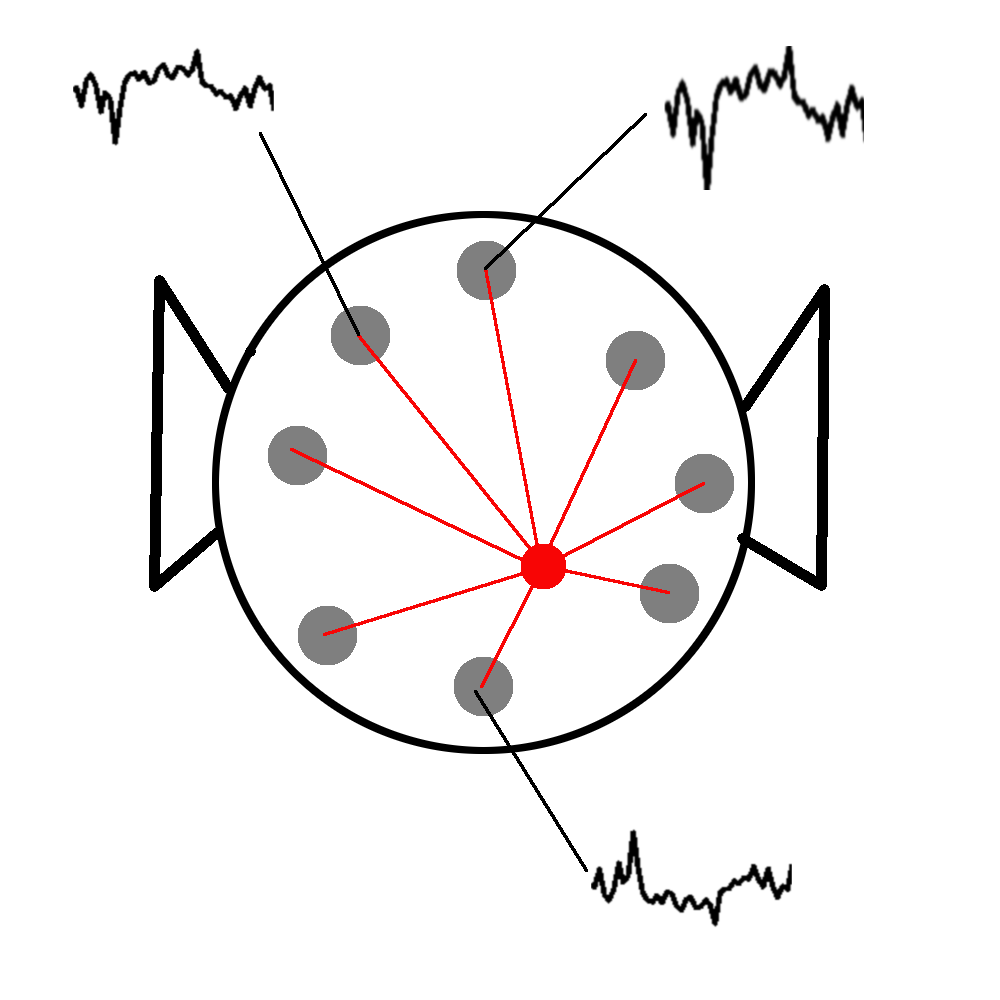
\includegraphics[width=.5\textwidth]{physic3}}%
	\only<4>{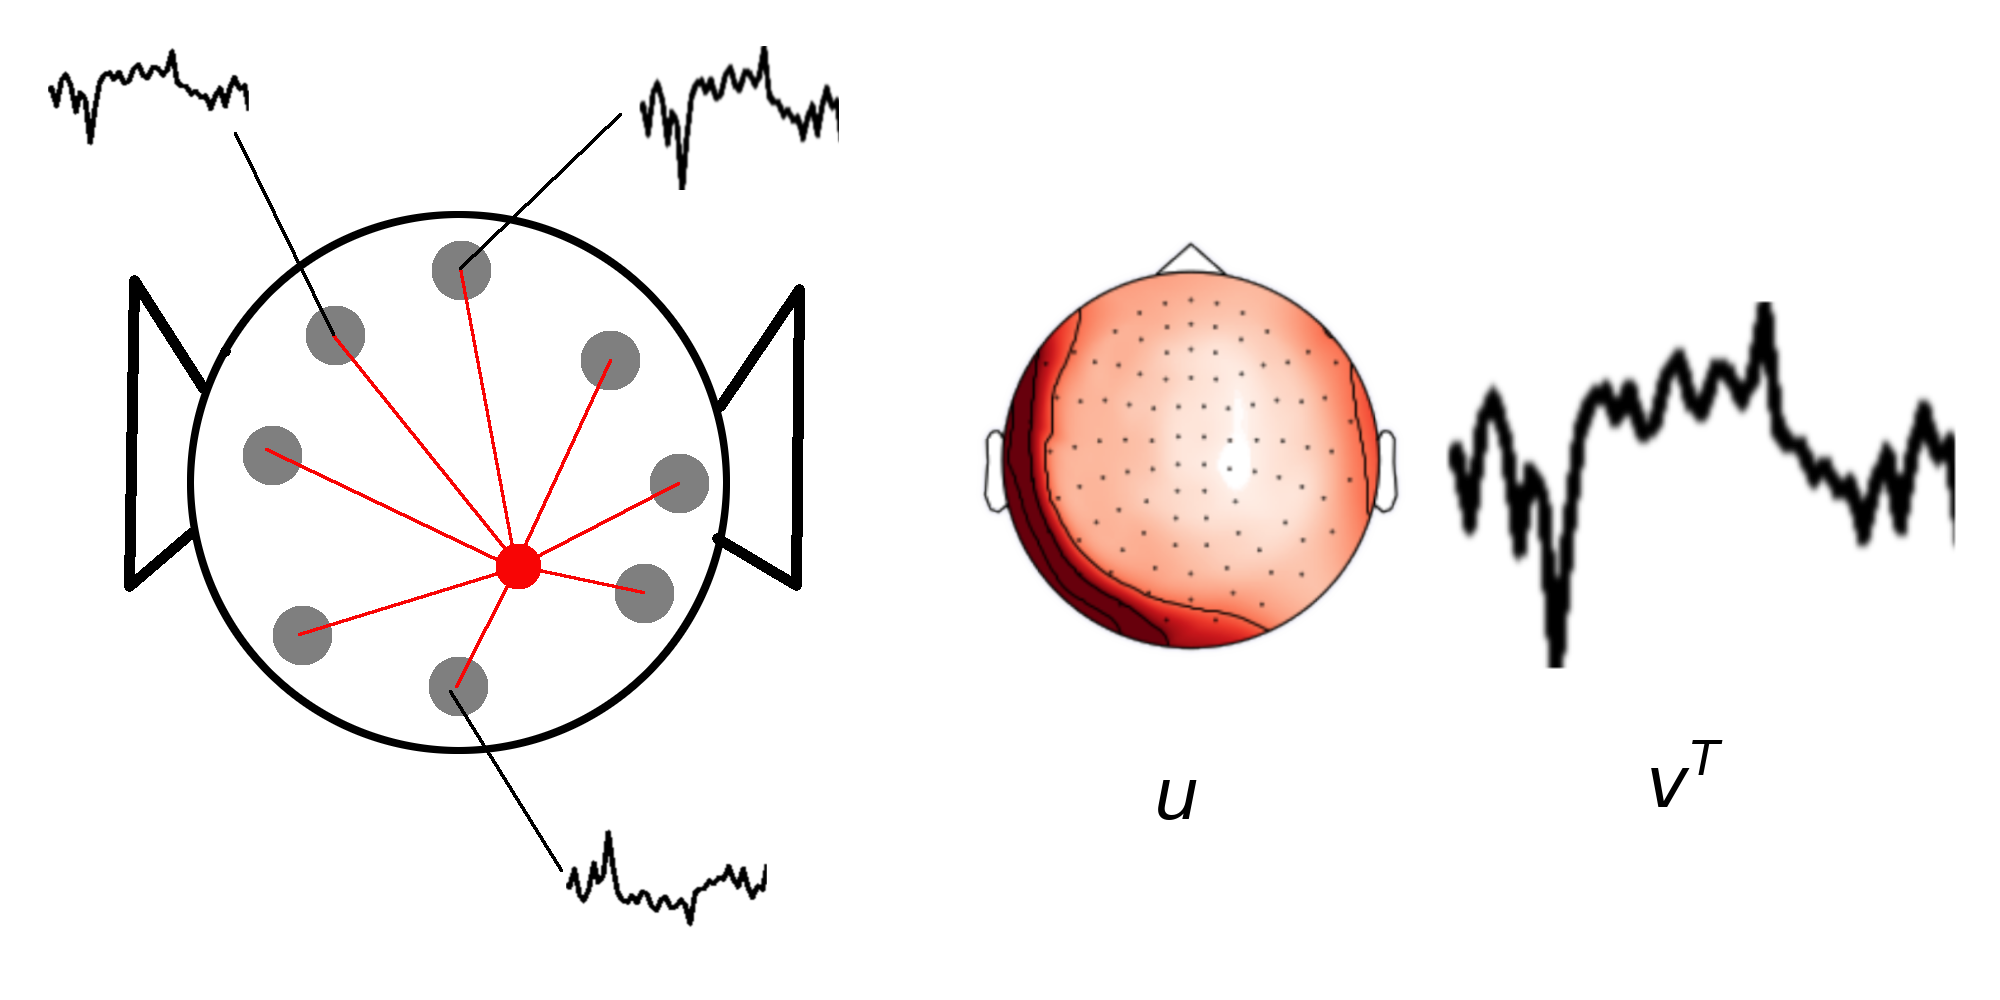
\includegraphics[width=\textwidth]{physic4}}
\end{frame}

\begin{frame}{Multivariate CSC with rank-1 constraint}
	\textbf{Idea}: Impose a rank-1 constraint on each dictionary atom $D_k$
	\vskip1em
	To make the problem tractable, use $u_k$ and $v_k$ \st{} $D_k = u_kv_k^\top$.

	\begin{equation}
	\label{eq:multichannel_csc}
	\begin{split}
	\min_{u_k, v_k, z_k^n} &\sum_{n=1}^N\frac{1}{2}\left\|X^n - \sum_{k=1}^K z^n_k * (u_k^{ } v_k^\top)\right\|_{2}^{2}
	+ \lambda  \sum_{k=1}^K \left\|z^n_k\right\|_1, \hspace{6pt}\\
	&\text{s.t. } ~~ \|u_{k}\|_2^2 \leq 1 \text{  , }\|v_{k}\|_2^2 \leq 1 \text{  and } z_k^n \geq 0~.
	\end{split}
	\end{equation}

	Here,
	\begin{itemize}
		\item $u_k \in \Rset^P$ is a spatial pattern
		\item $v_k \in \Rset^L$ is a temporal pattern
	\end{itemize}

    \strongpoint{This is a tri-convex problem}
\end{frame}

% \begin{frame}{Optimization strategy}
% \textbf{Tri-convex:} The problem is not jointly convex in $z^n_k$, $u_k$ and $v_k$ but it is convex in each block of coordinate.\\[1em]

% We can use a block coordinate descent, aka alternate minimization, to converge to a local minima of this problem. The 3 following steps are applied alternatively:

% \begin{itemize}
% 	\item \textbf{Z-step:} given a fixed estimate of the atom, compute the activation signal $z^n_k$ associated to each signal $X^n$.
% 	\item \textbf{u-step:} given a fixed estimate of the activation and temporal pattern, update the spatial pattern $u_k$.
% 	\item \textbf{v-step:} given a fixed estimate of the activation and spatial pattern, update the temporal pattern $v_k$.
% \end{itemize}
% \end{frame}

% \begin{frame}{Z-step: Locally greedy coordinate descent (LGCD)}

% $N$ independent problem such that
% \[
% 	\label{eq:sparse_code}
% 	\min_{z_k^n \ge 0} \frac{1}{2} \left\|X^n - \sum_{k=1}^K z_k^n * D_k\right\|_2^2
% 	+ \lambda\sum_{k=1}^K\left\|z_k^n\right\|_1~.
% \]
% This problem is convex in $z_k$ and can be solved with different techniques:
% \begin{itemize}
% 	\item Greedy CD \mycite{Kavukcuoglu2010}
% 	\item Fista \mycite{Chalasani2013}
% 	\item ADMM \mycite{Bristow2013}
% 	\item L-BFGS \mycite{Jas2017}
% \end{itemize}

% \strongpoint{These methods can be slow for long signals as the complexity of each iteration is at least linear in the length of the signal.}

% \end{frame}

\begin{frame}[t]{Z-step: Locally greedy coordinate descent (LGCD)}

	{\bf Coordinate Descent:} only 1 coordinate is updated at each iteration:\\
	\vskip.5em
	\begin{enumerate} % [<+->]
        \itemsep2em
		\item The coordinate $z_{k_0}[t_0]$ is updated to its optimal value $z'_{k_0}[t_0]$\\when all other coordinate are fixed.
		\item The updated coordinate is chosen\\[1em]

        \begin{itemize}\itemsep.5em
            \item Cyclic: $\mathcal{O}(1)$ \mycite{Friedman2007}
            \item Randomized: $\mathcal{O}(1)$ \mycite{Nesterov2010}
            \item Greedy: $\mathcal{O}(K\widetilde{T})$ \mycite{Osher2009}\\
            by maximizing $|z_k[t] - z'_k[t]|$\\
            \item Locally Greedy: $\mathcal{O}(K\widetilde{L})$ \mycite{Moreau2018}\\
            by maximizing $|z_k[t] - z'_k[t]|$ on a window
        \end{itemize}
    \end{enumerate}

\end{frame}



\begin{frame}{Locally Greedy Coordinate Descent \mycite{Moreau2018}}


We introduced the LGCD method which is an extension of GCD.\\
{
    \centering
    % \inputTikZ{.7}{tikz/LGCD}\\
}

\only<1-2>{
    \vskip1em
    GCD has $\mathcal O(K\widetilde{T})$ computational complexity.\\[1em]
    \only<2>{But the update itself has complexity $\mathcal O(KL)$}
}
%
\visible<3->{
    With a partition $\mathcal C_m$ of the signal domain $[1, K]\times [0, \widetilde{T}[$,
    \[
    \mathcal C_m = [1, K]\times [\frac{(m-1)\widetilde{T}}{M}, \frac{m\widetilde{T}}{M}[
    \]%
}%
\visible<4->{%
    The coordinate to update is chosen greedily on a sub-domain $\mathcal C_m$\\[1em]

    {\centering$\frac{\widetilde{T}}{M} = 2L-1~~\Rightarrow~~\mathcal O$(Coordinate selection) = $\mathcal O$(Coordinate Update)\\[1em]}

    The overall iteration complexity is $\mathcal O(KL)$ instead of $\mathcal O(K\widetilde{T})$.
    \begin{columns}
        \column{.5\textwidth}
        \strongpoint{Efficient for sparse $Z$}
        \column{.5\textwidth}
        \visible<5->{
        \strongpoint{Can be efficiently parallelized.}
        }
    \end{columns}
}


\end{frame}


\begin{frame}{D-step: solving for the atoms}

	We use the projected gradient descent with an Armijo backtracking line-search \cite{Wright1999} for both u-step and v-step for
	\begin{equation}
		\begin{split}
			\min_{\substack{\|u_{k}\|_2 \leq 1\\\|v_{k}\|_2 \leq 1}} E(u_k, v_k) \overset{\Delta}{=} \sum_{n=1}^N\frac{1}{2}\|X^n - \sum_{k=1}^K z^n_k * (u_k^{ }  v_k^\top) \|_{2}^{2} \hspace{6pt}
			\enspace .
		\end{split}
	\end{equation}

	One important computation trick is for fast computation of the gradient.
	\[
	\begin{split}
		\nabla_{u_k} E(u_k, v_k) &=  \nabla_{D_k}E(u_k, v_k) v_k ~~ \in \Rset^{P}~,\\
		\nabla_{v_k} E(u_k, v_k) &=  u_k^\top \nabla_{D_k} E(u_k, v_k)  ~~ \in \Rset^L~,
	\end{split}
	\]
	Computing $\nabla_{D_k} E(u_k, v_k)$ can be done efficiently
	\[
	\nabla_{D_{k}} E(u_k, v_k) =  \sum_{n=1}^N (z_k^n)^\Lsh * \left(X^n - \sum_{l=1}^K z^n_l * D_l\right)
	=  \Phi_k - \sum_{l=1}^K \Psi_{k, l} *  D_l \enspace ,
	\]

\end{frame}

% \begin{frame}{Pattern recovery}
% Test the pattern recovery capabilities of our method on simulated data,
% \[
% 	X^n = \sum_{k=1}^2 z_k * (u_kv_k^\top) + \mathcal E
% \]
% where $(u_k, v_k)$ are chosen patterns of rank-1 and the activated coefficient $z^n_k[t]$ are drawn uniformly and their value are uniform in $[0, 1]$.\\[1em]
% The noise $\mathcal E$ is generated as a gaussian white noise with variance $\sigma$.\\[1em]

% We set $N=100$, $L=64$ and $\widetilde{T}=640$
% \end{frame}

\begin{frame}{Pattern recovery}
Patterns recovered with $P = 1$ and $P=5$. The signals were generated with the two simulated temporal patterns and with  $\sigma = 10^{-3}$. \\[1em]
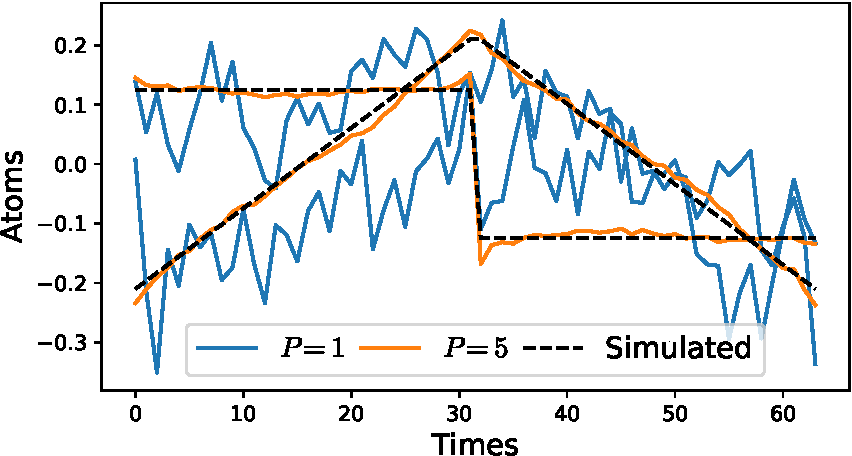
\includegraphics[width=\textwidth]{1D_vs_multi_uv_hat_P5.pdf}
\end{frame}
\begin{frame}{Pattern recovery}
Evolution of the recovery loss with $\sigma$ for different values of $P$. Using more channels improves the recovery of the original patterns.\\[1em]
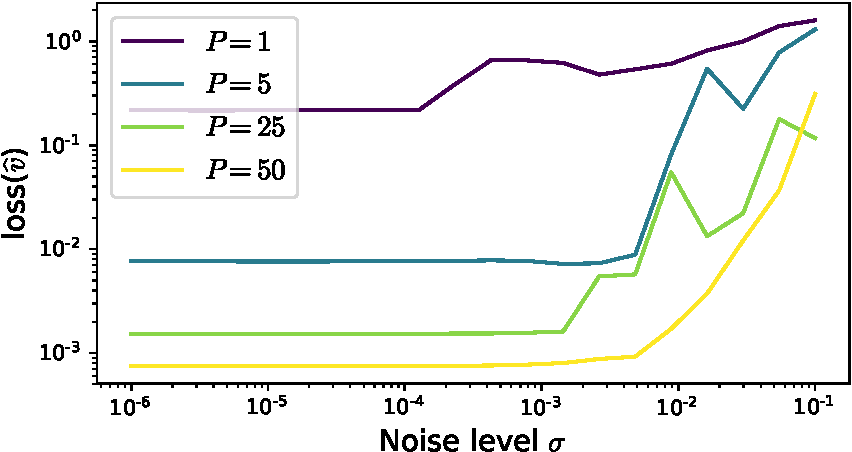
\includegraphics[width=\textwidth]{1D_vs_multi.pdf}
\end{frame}


\begin{frame}{MNE sample data}
A selection of temporal waveforms of the atoms learned on the MNE sample dataset.\\[1em]
\centering
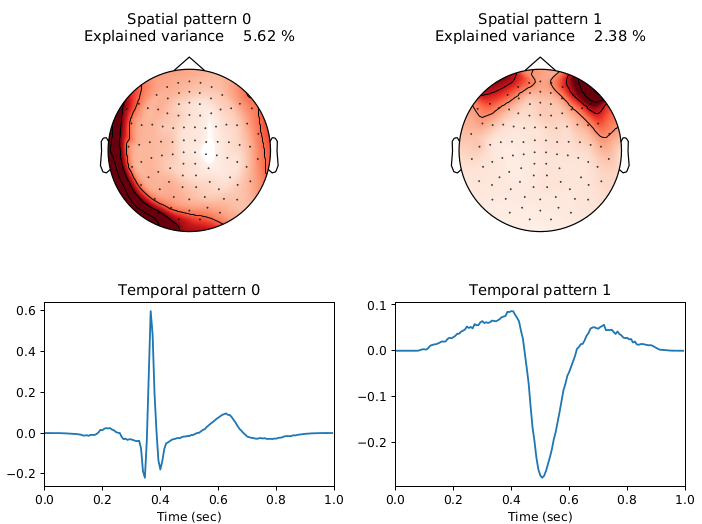
\includegraphics[height=0.7\textheight]{artifacts}
\end{frame}


\frame[t]{
    \frametitle{Learned atoms -- Evoked response}

    \centering
    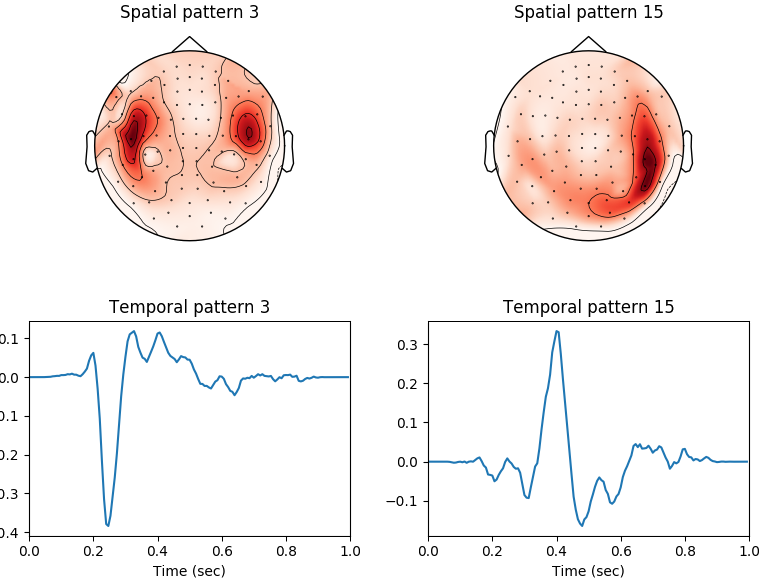
\includegraphics[width=.9\columnwidth]{evoked}
}


\frame[t]{
    \frametitle{Learned atoms -- Induced responses}

    \centering
    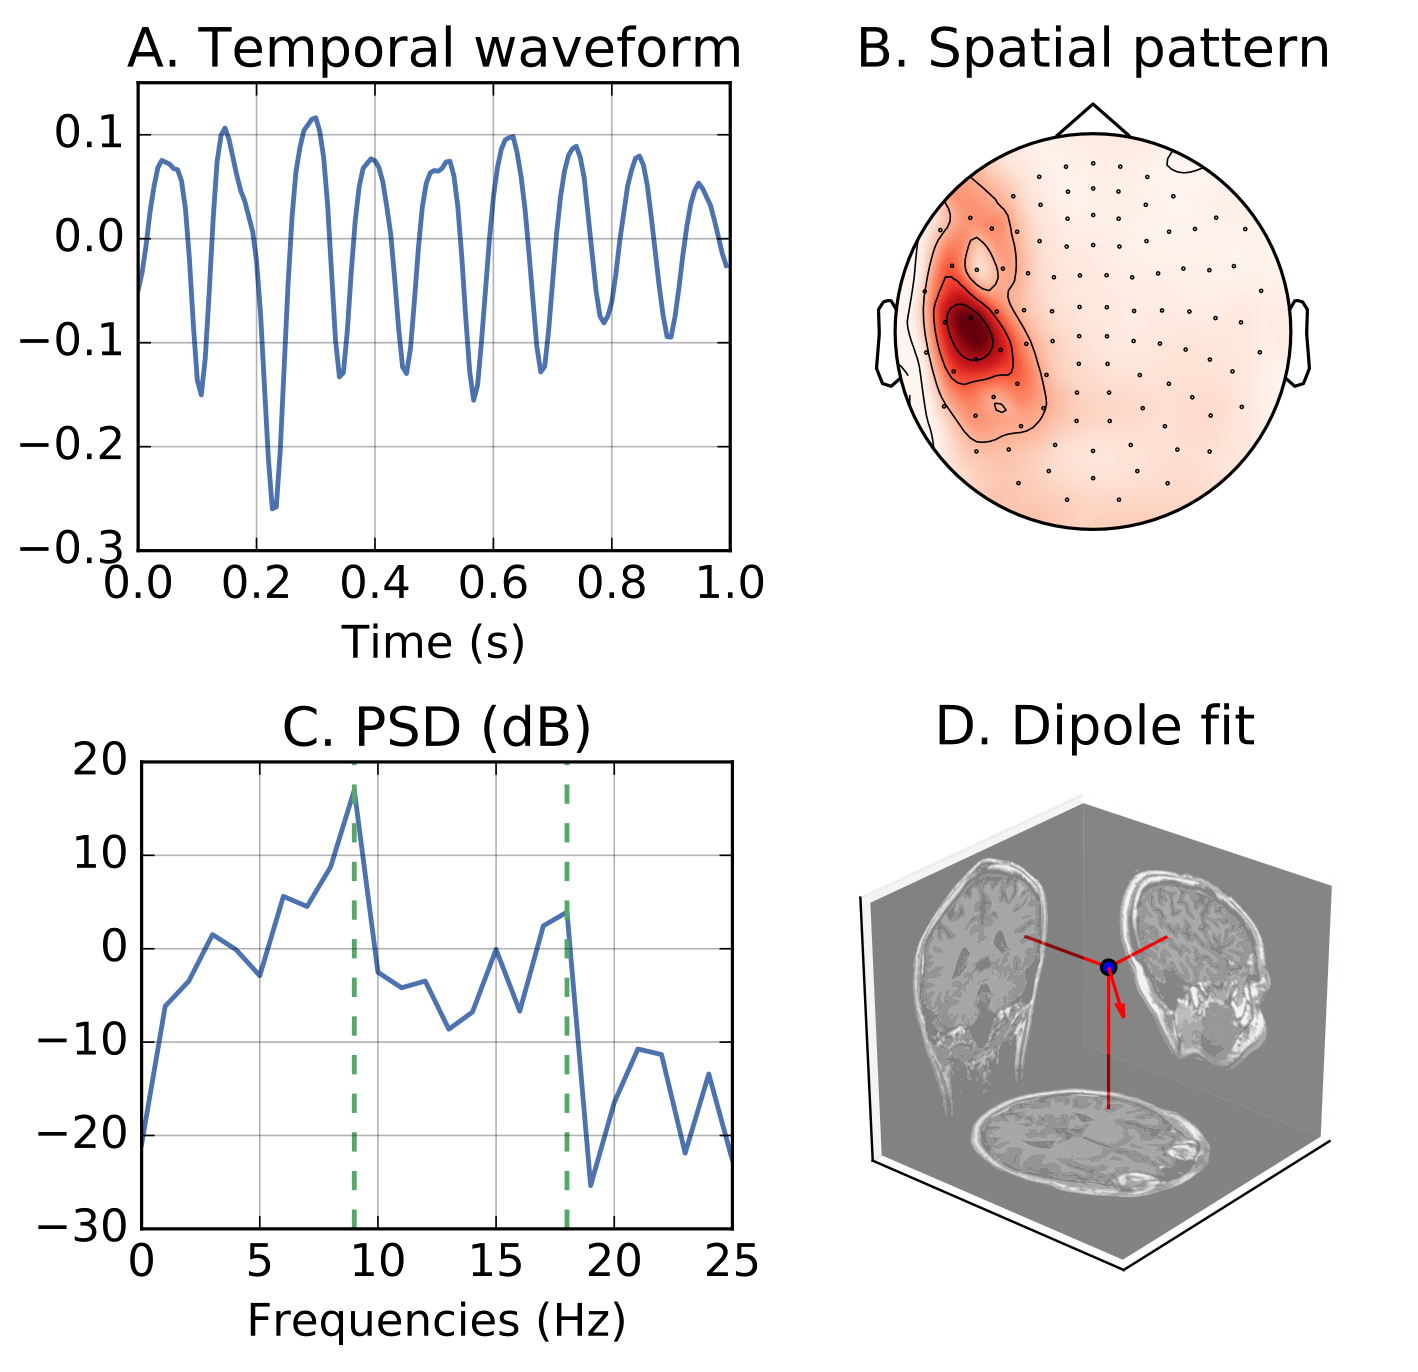
\includegraphics[width=.7\columnwidth]{atom_somato}
}


{\usebackgroundtemplate{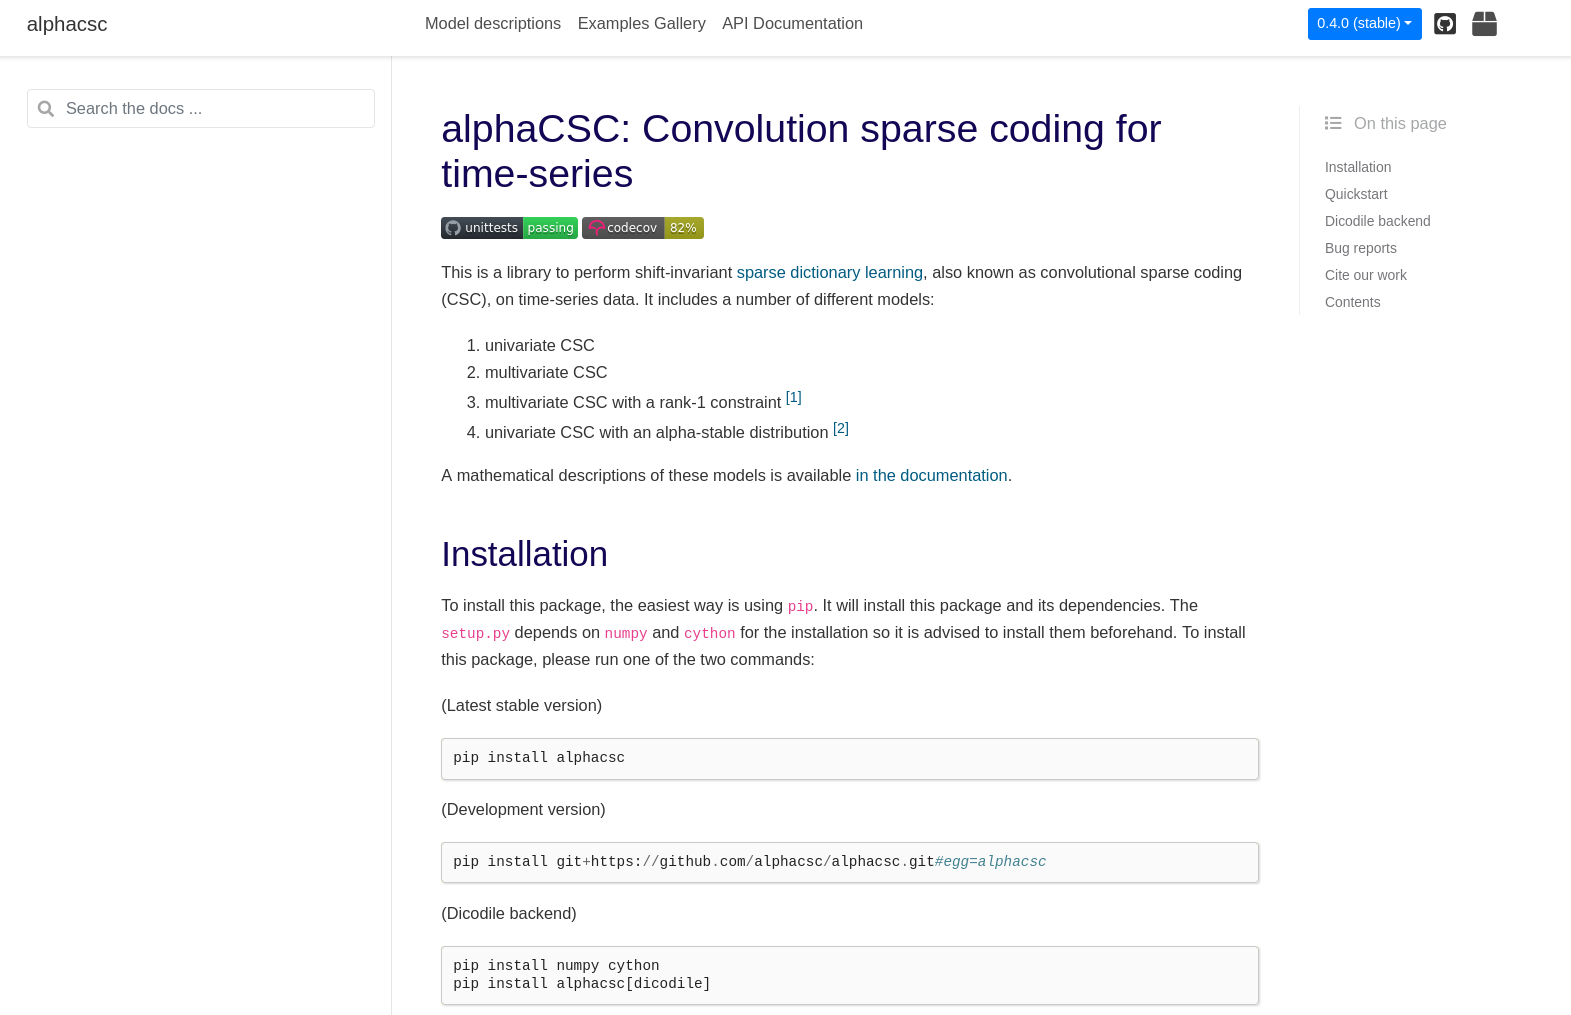
\includegraphics[width=\paperwidth]{alphacsc_04}}%
\frame{
    \begin{columns}
        \column{.5\textwidth}
        \column{.4\textwidth}
        \highlightbox{Python code online:\\
                        https://alphacsc.github.io\\[1em]
                        \texttt{pip install alphacsc}}
        \vskip2em
            \highlightbox{Examples reproduce figures from this talk!}

    \end{columns}
}}


\section{Modeling stimuli induced patterns\\with Point Processes}

\parttitleframe{Allain2022}

\frame{
    \frametitle{Stimuli Induced Patterns}

    \myitem{} Manual pattern identification\\[.5em]
    \myitem{} No quantification of how stimuli influence patterns activation.\\[1em]

    \centering
    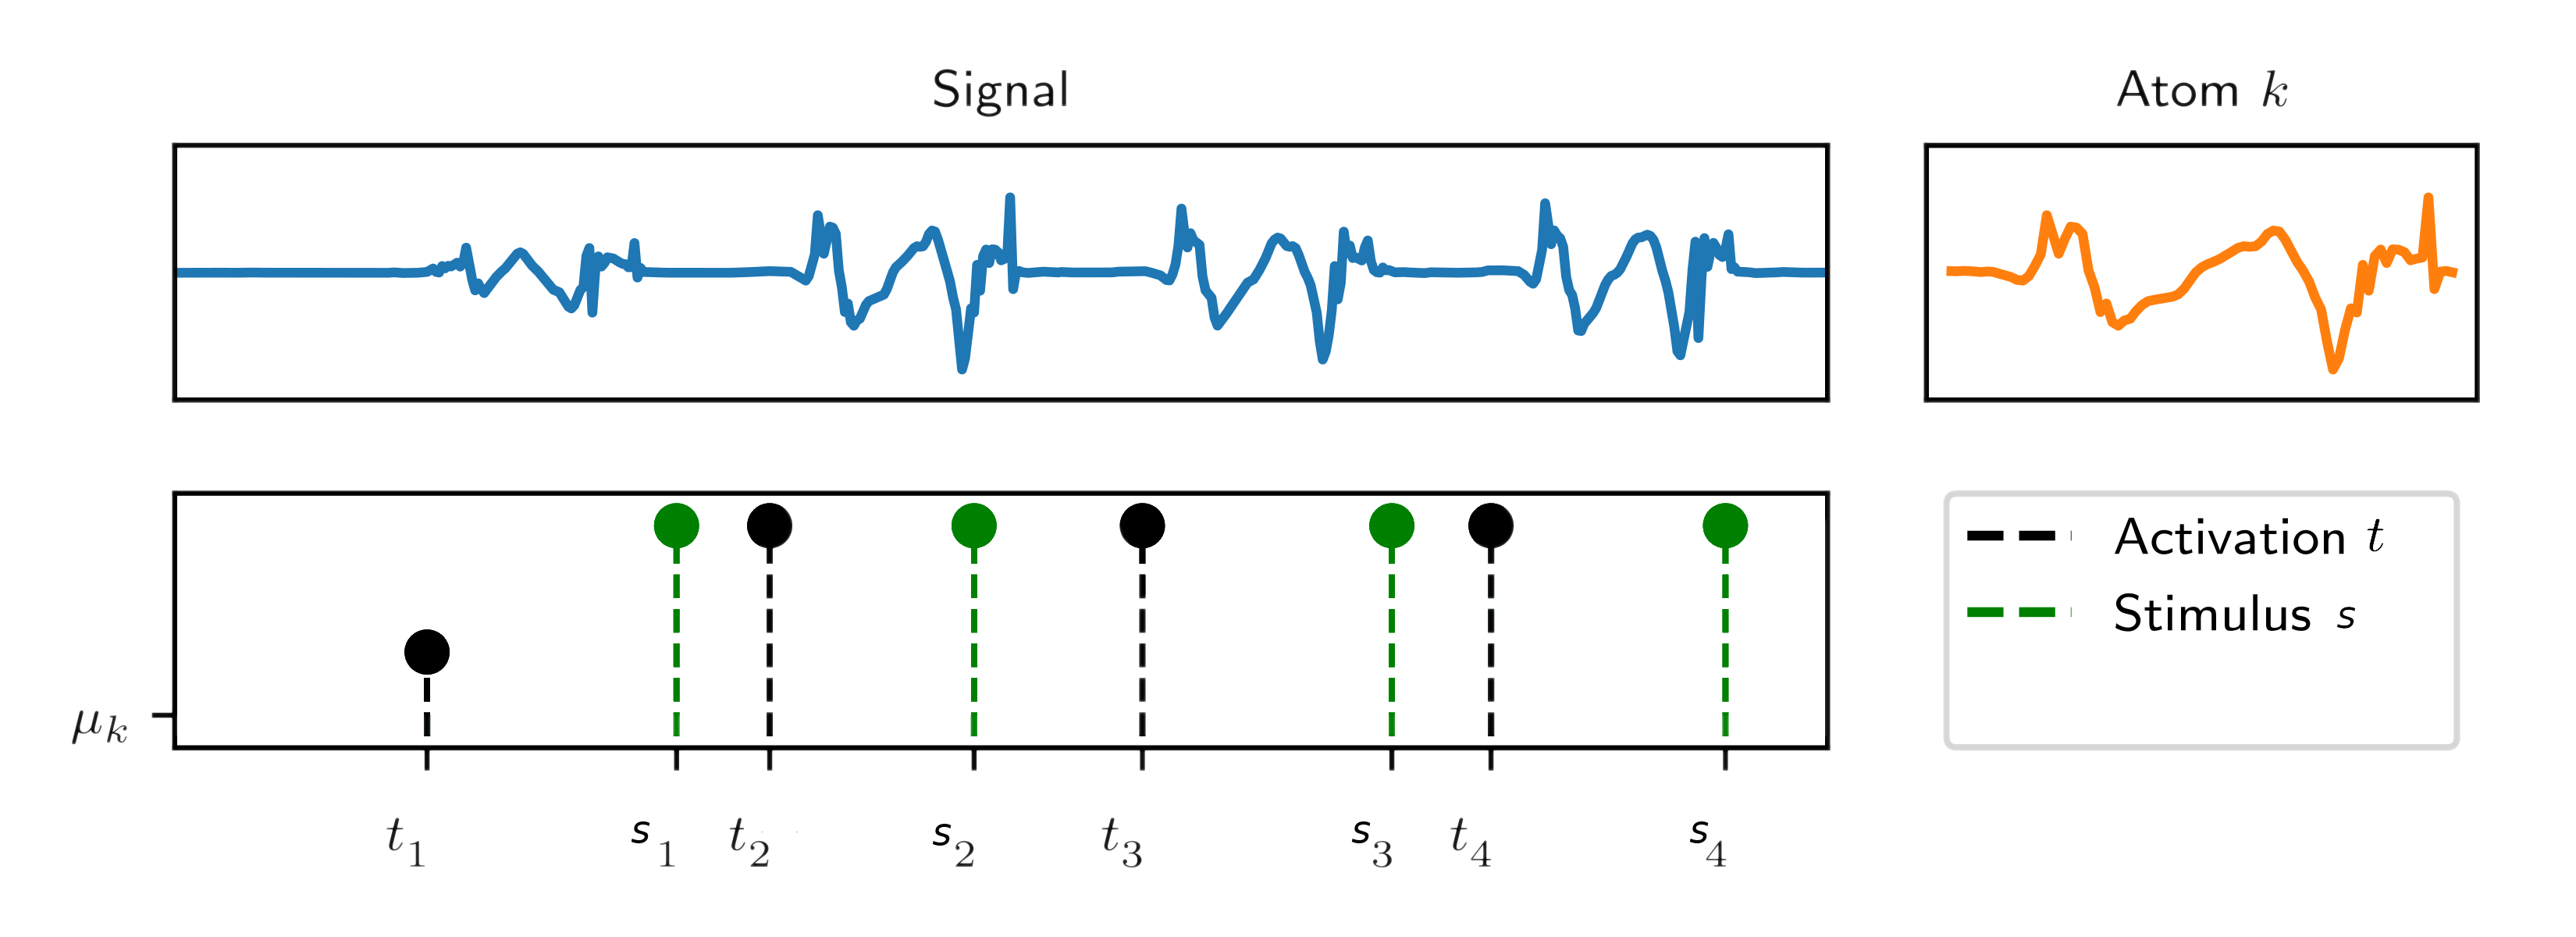
\includegraphics[width=\textwidth]{csc_and_pp_no_intensity.png}\\[1em]


    Activations and stimuli can be seen as \emph{Point Processes}.\\
}

\frame{
    \frametitle{Point Processes \mycite{Daley2003}}

    \begin{itemize}\itemsep.5em
        \item Stochastic model for stream of events
        \item Time of arrival $\{t_k\}$ associated with counting process $N(t)$
        \item Characterized by the intensity:
        \[
            \lambda(t | \mathcal F_t) = \lim_{dt \to 0} \frac{P(N(t+dt) - N(t) = 1 | \mathcal F_t)}{dt}
        \]
    \end{itemize}

    \begin{columns}
        \column{.5\textwidth}
            \centering
            Poisson process with constant probability of arrival
            \[
                \lambda(t) = \mu_0
            \]
        \column{.5\textwidth}
        {\centering
        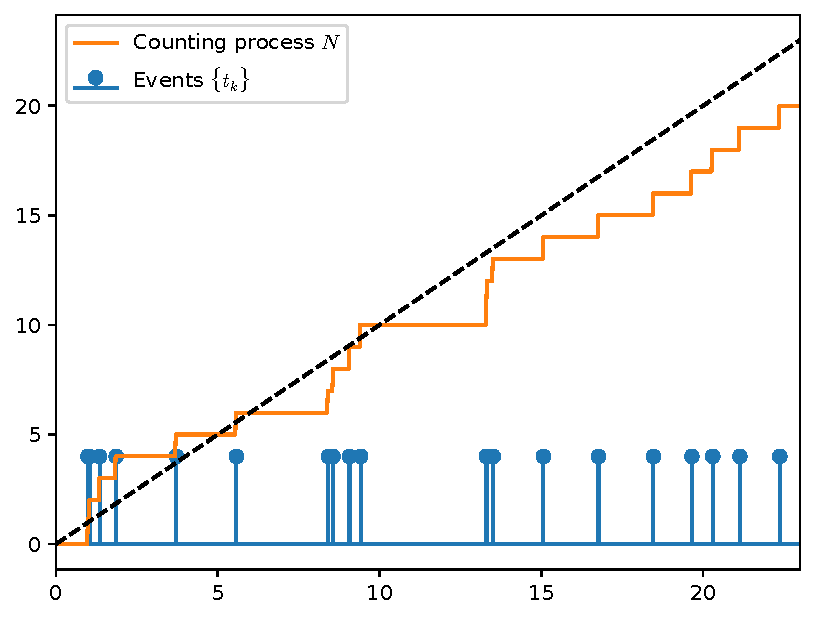
\includegraphics[width=\textwidth]{point_process}\\}
    \end{columns}
}

\frame{
    \frametitle{DriPP -- Driven Point Process}

    {\bf Idea:} Model the intensity of the activation $\{t_k\}$ depending on the PP from the stimuli $\{s_p\}$.
    \[
        \lambda(t | \mathcal F_t) = \lambda(t | \{s_p; s_p < t\}) = \mu_0 + \sum_{s_p < t} \kappa(t - s_p)
    \]

    \centering
    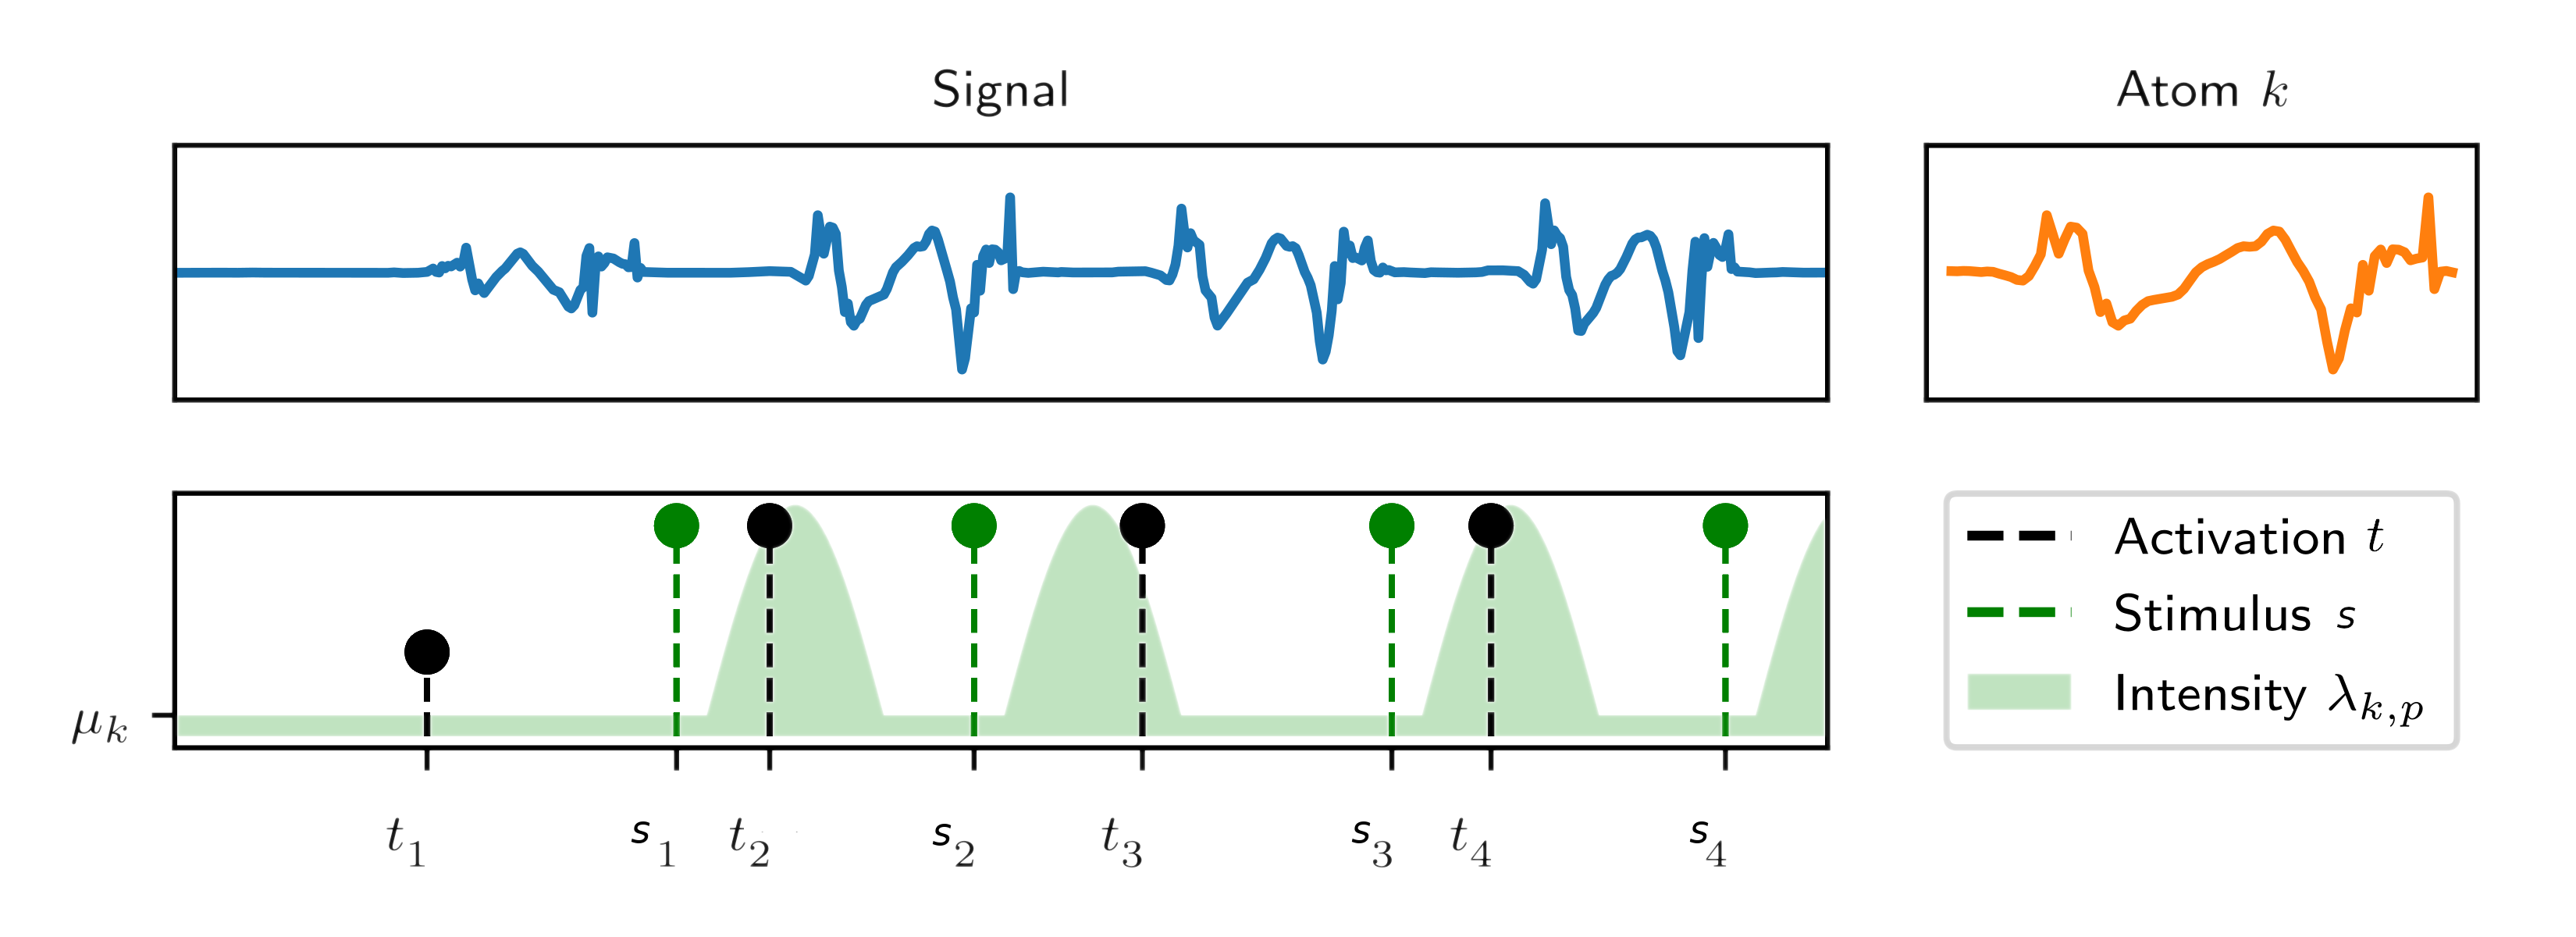
\includegraphics[width=\textwidth]{csc_and_pp.png}\\[1em]


    % Activations and stimuli can be seen as \emph{Point Processes}.\\
}

\frame{
    \frametitle{Modeling latency}

    Chosing a model for stimuli based modeling:
    \[
        \lambda(t | \mathcal F_t) = \mu_0 + \sum_{s_p < t} \alpha\kappa(t - s_p)
    \]

    \begin{columns}

        \column{.5\textwidth}
        \begin{itemize}
            \item $\mu_0 \ge 0$: spontaneous activity.
            \item $\alpha \ge 0$: allow for stimuli to have no effect.
            \item $\kappa(\tau)$: pdf of a truncated Gaussian $\mathcal N(m, \sigma^2)$ to model latency.
        \end{itemize}
        \column{.5\textwidth}
        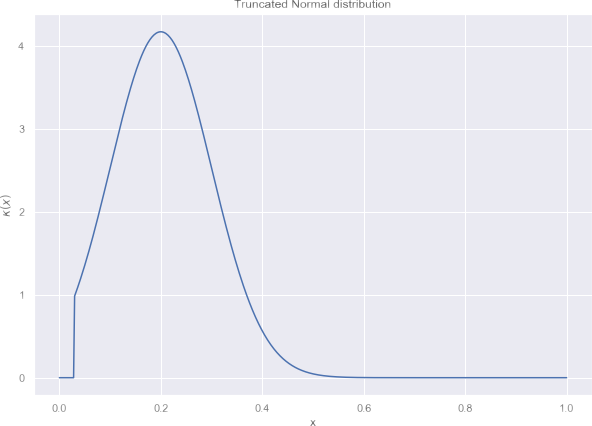
\includegraphics[width=\textwidth]{trunc_norm_distribution}
    \end{columns}
}

\frame{
    \frametitle{Parameters estimation}

    The negative log-likelihood of the model can be computed using the intensity $\lambda$:
    \begin{align*}
        \mathcal L(\{t_k\}; \Theta) &= \int_0^T \lambda(t ) dt -\sum_{t_k} \lambda(t_k)\\
        & = \mu_0 T + \alpha |\{t_k\}| - \sum_{t_k} \log(\mu_0\sum_{s_p < t_k} \alpha\kappa(t_k - s_p))
    \end{align*}
    with $\Theta = (\mu_0, \alpha, m, \sigma^2)$\\[1em]

    \strongpoint{Parameter estimation is done using an EM algorithm.}
}


\frame{
    \frametitle{Parameters recovery}

    Events simulated with the Truncated Gaussian model:
    {\centering
    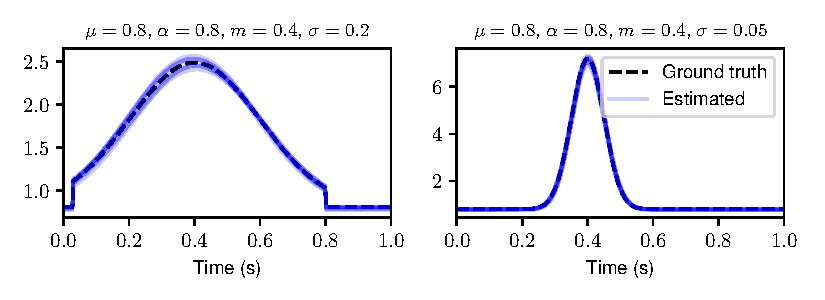
\includegraphics[width=.8\textwidth]{kernel_recovery}\\
    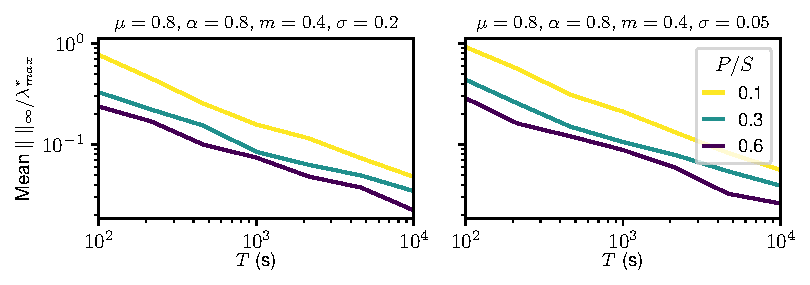
\includegraphics[width=.8\textwidth]{mean_recovery}\\
    }
}


\frame{
    \frametitle{Results for artifacts and evoked atoms - samples}

    {\centering
    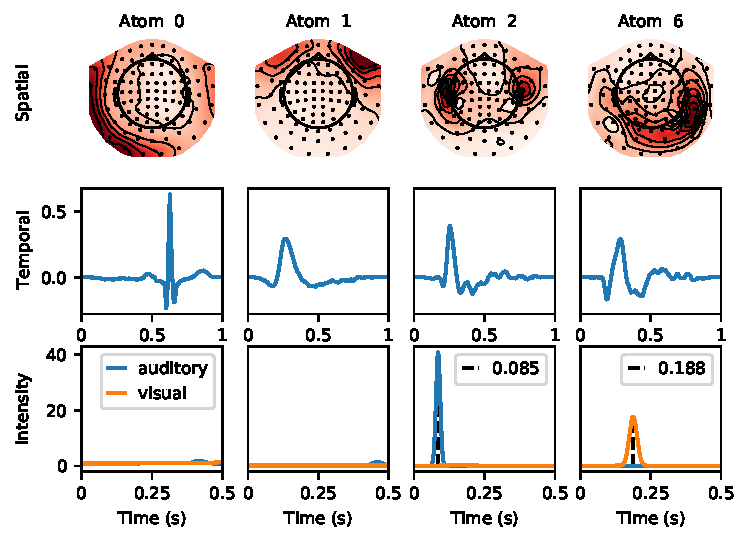
\includegraphics[width=.8\textwidth]{atom_evoked_sample}\\
    }
}


\frame{
    \frametitle{Results for artifacts and evoked atoms - somato}

    {\centering
    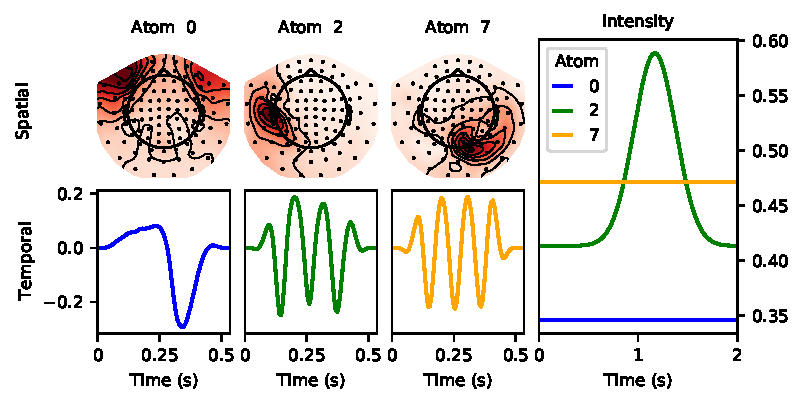
\includegraphics[width=.8\textwidth]{atom_induced_somato}\\
    }
}


\frame{
    \frametitle{Results for artifacts and evoked atoms - somato}

    {\centering
    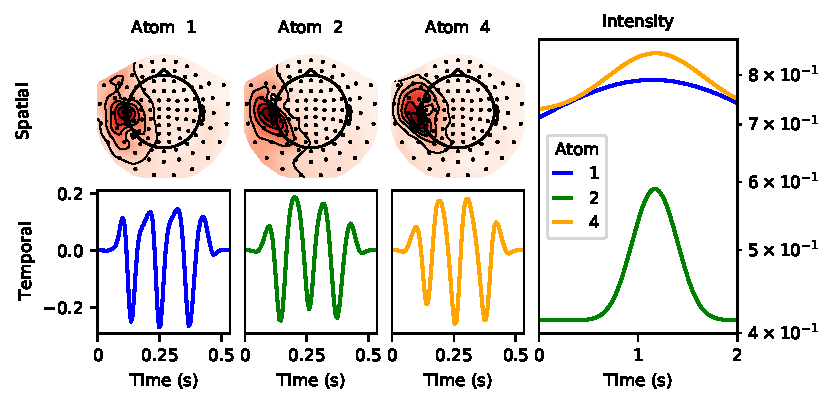
\includegraphics[width=.8\textwidth]{atom_induced_somato_wave}\\
    }
}

\frame{
    \frametitle{Conclusion}

    \begin{itemize}\itemsep1em
    \item CDL can learn recurring patterns in multivariate signals.
    \item Converts the signal into a stream of events.
    \item PP framework can model the activation distribution.
    \end{itemize}

    \vskip2em
    {\bf Limitations and on-going work:}\\[1.5em]
    \begin{itemize}\itemsep1em
        \item Not easy to apply to population level.
        \item DriPP does not model inhibition.
        \item CDL and PP are separated.
    \end{itemize}
}




    \frame{
        \frametitle{Learning a linear ML model}


        \textbf{Setup:}\\[1em]
        \begin{itemize}
            \item Binary classification task $(X_i, y_i)_{i=1}^N \in \mathbb R^p \times \{-1, 1\}$
            \item Linear model: predict $y$ from $X$ with $\text{sign}(\langle \theta, X\rangle)$.
        \end{itemize}

        {\centering
        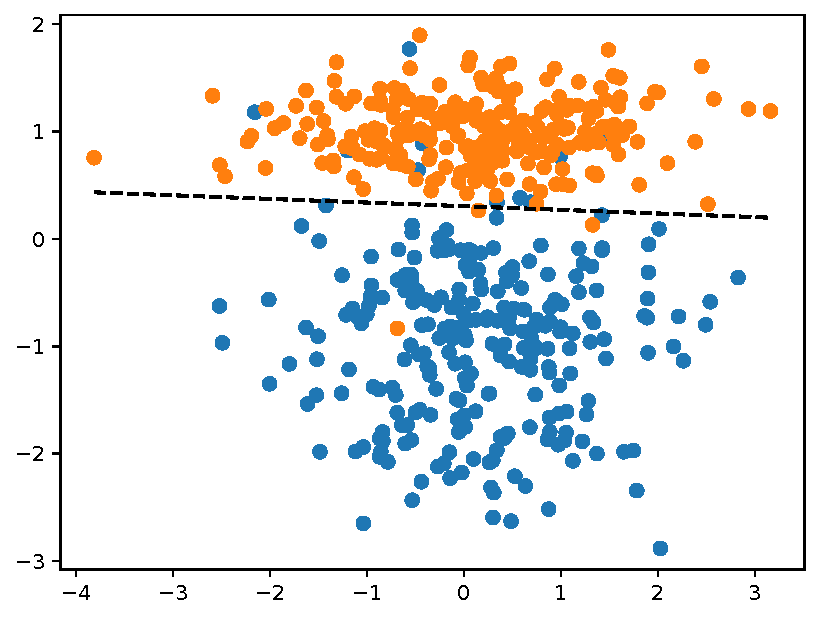
\includegraphics[width=.6\textwidth]{images/logreg_noreg}\\
        }

    }

    \frame{
        \frametitle{Learning a linear ML model}

        \textbf{Logistic loss:}\\[1em]

        \[
            G(\theta) = \frac1N \sum_{i=1}^N \log( 1 + e^{-y_i \langle \theta, X_i\rangle})
        \]


        \textbf{Training the model:}\\[1em]
        \[
            \theta^* = \argmin_\theta G(\theta)
        \]

    }

    \frame{
        \frametitle{Avoiding overfitting}

            Here, the second feature is uninformative,\\[2em]

            {\centering
            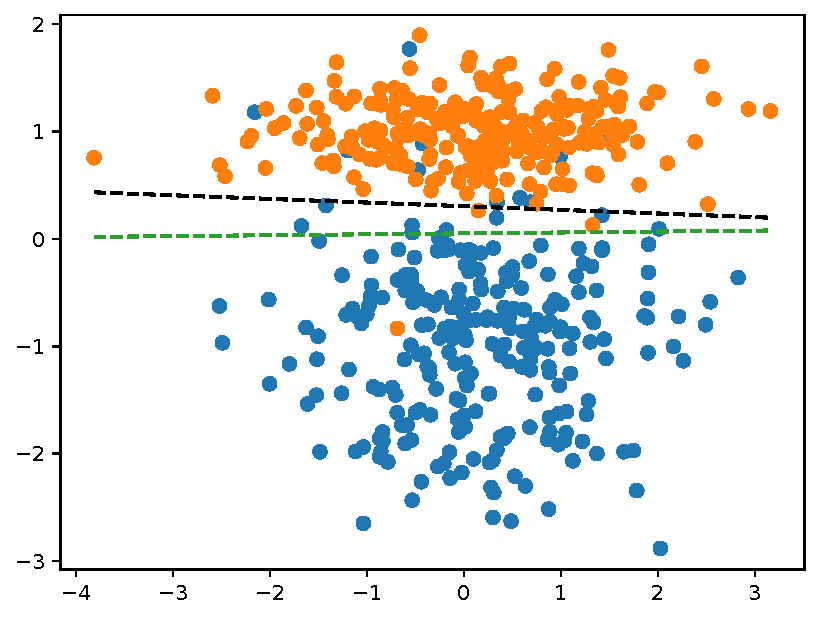
\includegraphics[width=.6\textwidth]{images/logreg_reg}\\
            }
    }
    \frame{
        \frametitle{Avoiding overfitting with a regularization}
        \textbf{\textcolor{blue!70}{Regularized} Logistic loss:}

        \[
            G(\theta, \lambda) = \frac1N \sum_{i=1}^N \log( 1 + e^{-y_i \langle \theta, X_i\rangle}) + \color{blue!70}\lambda\|\theta\|_2^2
        \]


        \textbf{Training the model:}\\[1em]
        \[
            \theta^*({\color{blue!70}\lambda}) = \argmin_\theta G(\theta,{\color{blue!70} \lambda})
        \]

        \pause
        \strongpoint{\bf \Large How to choose $\lambda$?}

    }

    \frame{
        \frametitle{Evaluating the generalization}

        We want to find $\lambda$ that ensure the best \emph{generalization} of $\theta^*(\lambda)$.\\[2em]

        \textbf{Validation loss:} use held out data $(X^{\it val}_i, y^{\it val}_i)_{i=1}^M$
        \[
            F(\theta) = \frac1M \sum_{i=1}^M \log( 1 + e^{-y^{\it val}_i \langle \theta, X_i^{\it val}\rangle})
        \]

        Independent estimate of the risk of the model.\\[1em]

        \pause
        \strongpoint{Find $\lambda$ that gives a model $\theta^*(\lambda)$ with a good validation loss.}
    }

    \frame{
        \frametitle{The Grid Search}

        \begin{itemize}\itemsep1.5em
            \item Select a grid of parameters $\{\lambda_1,\dots \lambda_K\}$.
            \item Train a model for each parameter $\lambda_k$: $\theta^*(\lambda_k)$.
            \item Evaluate the performance with the validation loss $F(\theta^*(\lambda_k))$.
            \item Keep the value $\lambda_k$ with the best performance.
        \end{itemize}

        \pause
        \vskip2em
        \textbf{Mathematical rewritting:}
        \[\begin{cases}
            \quad\min_{\lambda \in \{\lambda_1,\dots \lambda_K\}}
            F(\theta^*(\lambda))\\
            s.t.\quad \theta^*(\lambda) = \argmin_\theta G(\theta, \lambda)
        \end{cases}\]
    }

    \frame{
        \frametitle{The Grid Search with multiple hyperparameters}

        \textbf{Regularized Logistic loss:}

        \[
            G(\theta, \lambda) = \frac1N \sum_{i=1}^N \log( 1 + e^{-y_i \langle \theta, X_i\rangle}) + \alt<2->{\color{blue!70}\sum_{k=1}^p\lambda_k\theta_k^2}{\lambda\|\theta\|_2^2}
        \]

        \visible<2->{
            Grid search is inefficient as the grid increases exponentially with the number of parameters.
        }
        \vskip2em

        \visible<3>{
            \strongpoint{\bf\large Can we use first-order methods to minimize $h(\lambda) = F(\theta^*(\lambda))$?}
        }
    }

    \frame{
        \frametitle{Bi-level optimization}

        {\bf Bi-level problem:} Optimization problem with two levels\\[1em]
        \begin{align*}
            \min_\lambda ~& {\color{darkblue} h(\lambda)} = {\color{darkred}F(\lambda, \theta^*(\lambda))} \\[.5em]
                & s.t.\quad \theta^*(\lambda) = \argmin_\theta {\color{lightgreen}G(\lambda, \theta)}
        \end{align*}
        \begin{tikzpicture}[overlay]
            \draw[<-, thick, shorten >=8, darkblue] (4.1, 1.7) -- +(-1.5, -1.3) node[darkblue] {\emph{Value function}};
            \draw[<-, thick, shorten >=35,darkred] (7.3, 1.9) -- +(3, -.2) node {\emph{\color{darkred}Outer function}};
            \draw[<-, thick, shorten >=8, lightgreen] (8, .5) -- +(0, -.8) node {\emph{\color{lightgreen} Inner function/Problem}};
        \end{tikzpicture}

        \vskip3em
        {\bf Goal:}  Optimize the value function $h$ whose value depends on the result of another optimization problem.
    }
    \frame[t]{
        \frametitle{Bi-level optimization problems: Model selection}

        \vskip1em
        {\bf Selecting the best model:}\\[.5em]
        \begin{itemize}\itemsep.7em
            \item $G$ is the training loss and $\theta$ are the parameters of the model.
            \item Select the hyper-parameter $\lambda$ to get the best validation loss $F$.
        \end{itemize}
        \vskip1em
        \alt<2->{
            \alt<3>{
                {\bf Neural Architecture Search:} $\lambda$ parametrizes the architecture. \\

                {\centering
                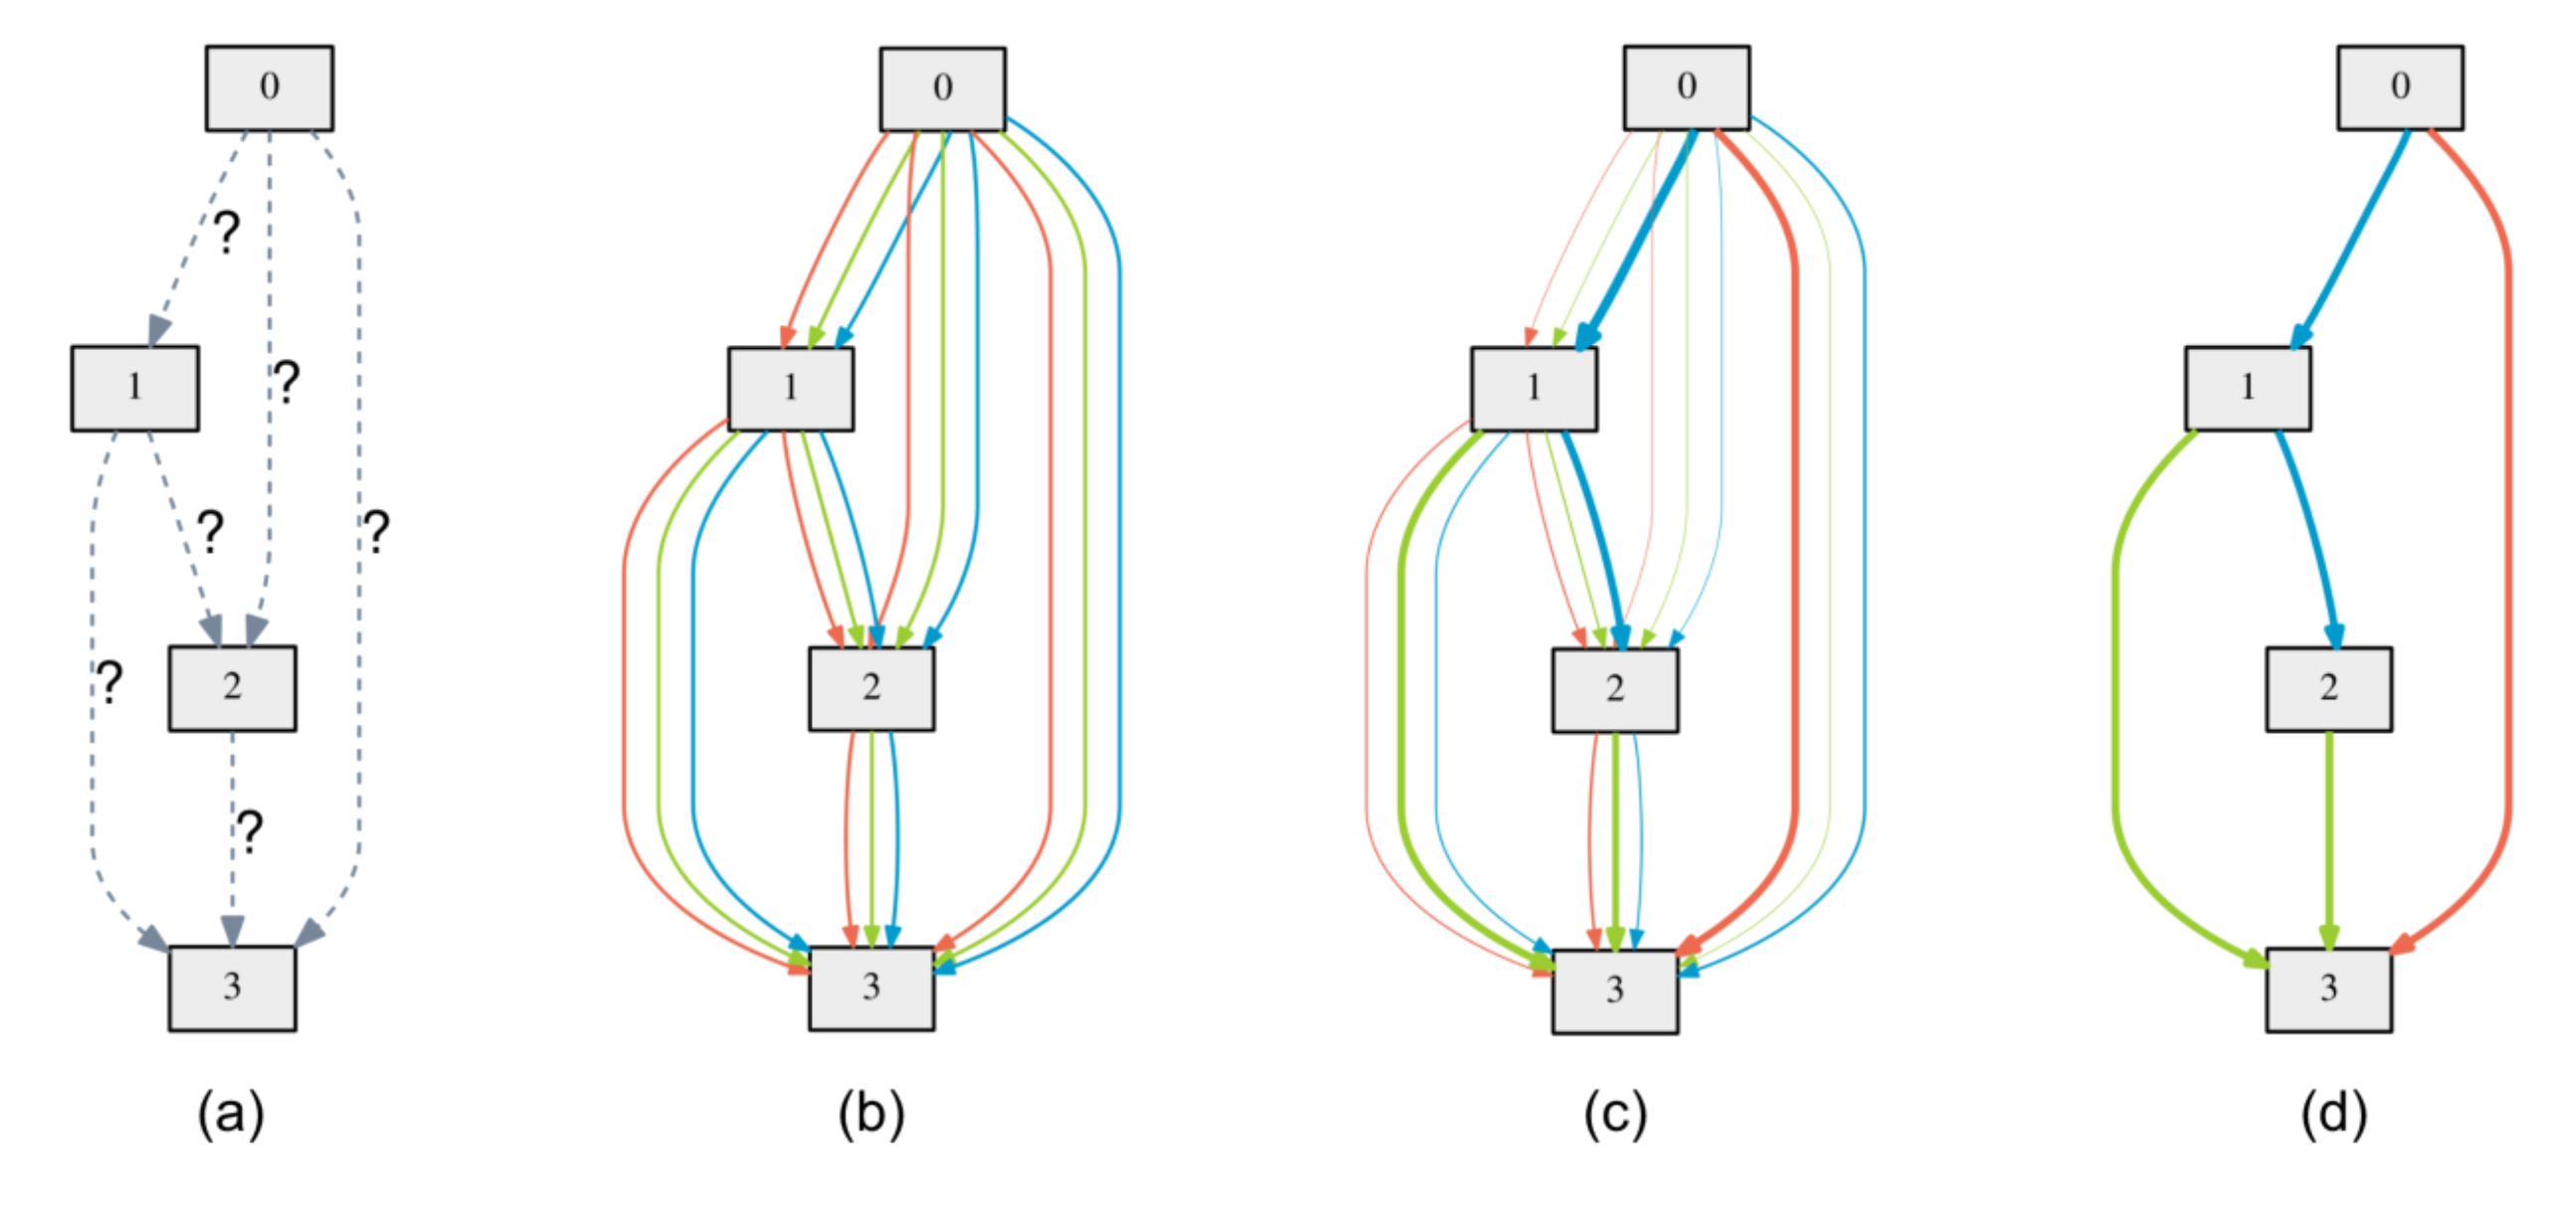
\includegraphics[width=.8\textwidth]{darts.png}\\
                }

            }{
                {\bf Data augmentation:} $\lambda$ parametrizes the transformations distribution. \\

                {\centering
                \includegraphics[]{data_aug.png}\\
                }
            }
        }{
            {\bf Hyperparameter optimization:} $\lambda$ is a regularization parameter:\\[1em]

            {\centering
            \includegraphics[width=.4\textwidth]{images/logreg_reg}\\
            }
        }

        % \begin{itemize}
        %     \item \emph{Hyperparameter optimization:}
        %         $\lambda$ are the regularisation parameters,\\
        %         or the number of trees, \dots\\
        %         \rightcite{Pedregosa 2016, Lorraine et al. 2020}
        %     \item \emph{Automatic Data Augmentation:} $\lambda$ are the parameters of data augmentation used to train the model.\\
        %     \rightcite{Cubuk et al. 2019; Rommel et al. 2022}
        %     \item \emph{Neural Architecture Search:} $\lambda$ are the parameter of a Neural Network architecture.\\
        %     \rightcite{Liu et al. 2018, Zhang et al. 2021}
        % \end{itemize}

    }


    \frame{
        \frametitle{Bi-level optimization problems: Implicit Deep Learning}

        {\bf Deep Equilibrium Network:}
        \[
            \begin{cases}
            \min_\lambda h(\lambda) = \frac1N\sum_{i=1}^N \mathcal L(y_i, \theta^*(X_i, \lambda))\\
            s.t.\quad \theta^*(X_i, \lambda) = g_\lambda(\theta^*(X_i, \lambda))
            \end{cases}
        \]
        Output of the network is the root of $G(\theta, \lambda) = \theta - g_\lambda(\theta) =0$.\\[2em]

        \begin{columns}
            \column{.4\textwidth}
            \myitem{} {\bf Mimic infinite depth:}
            \[
                \theta^{(t+1)} = g_\lambda(\theta^{(t)})\quad t\to\infty\enspace .
            \]
            \myitem{} {\bf Efficient memory}\\
            \myitem{} {\bf Slow runtime}
            \column{.5\textwidth}
            {\centering
                \includegraphics[width=.9\textwidth]{deq_memory.png}\\
            }
        \end{columns}
    }

    \frame{
        \frametitle{Solving bi-level optimization}

        \alt<2>{
            \vskip2em
            \underline{\bf First order methods:} Gradient descent on $h$
            \begin{columns}
                \column{.5\textwidth}
                \vskip1em
                Iterate in the steepest direction:
                $$
                    \lambda^{t+1} = \lambda^t - \rho^t \nabla h(\lambda)
                $$
                \myitem{} Gradient $\nabla h(\lambda) = \frac{d\; F(\lambda, \theta^*(\lambda))}{d\;\lambda}$\\[.5em]
                \myitem{} Step size $\rho^t$.
                \column{.5\textwidth}
                \includegraphics[width=\textwidth]{gd_Steps.png}
            \end{columns}
        }{
            \underline{\bf Black box methods:} Take $\{\lambda_k\}_k$ and compute $\min_k h(\lambda_k)$ \\[1em]
            {
                \centering
                \myitem{} Grid-Search
                \hskip4ex
                \myitem{} Random-Search
                \hskip4ex
                \myitem{} Bayesian-Optimization\\[1em]
            }
            \strongpoint{Do not scale well with the dimension}

        }

        % \pause
        % \begin{itemize}
        %     \item Can we compute the gradient of $h$?
        %     \item Do we need to compute $\theta^*(\lambda)$?\\
        %     \item How to efficiently approximate $\nabla h(\lambda)$?
        % \end{itemize}
    }

    % \frame{
    %     \frametitle{Some challenges?}


    %     \begin{itemize}\itemsep1em
    %         \item Computing the gradient of $h$?\\
    %         \rightcite{Implicit function theorem}
    %         \item Do we need to compute $z^*$?\\
    %         What is the best gradient estimate with $z_t$?\\
    %         \rightcite{Pedregosa 2016, Ablin et al. 2020, Malezieux et al. 2022}
    %         \item How to efficiently compute the implicit gradient?\\
    %         \rightcite{Lorraine et al. 2017, Ramzi et al. 2022}
    %         \item How to use stochastic methods?
    %         \rightcite{Grazzie et al. 2021, Chen et al. 2021}
    %     \end{itemize}
    % }


    % \section{Implicit Gradient}
    % \parttitleframe[Computing the gradient of the value function $h$]{Pedregosa2016,Lorraine2020,Ramzi2022}

    \frame{
        \frametitle{Computing the gradient of $h$}

        \underline{\bf{Value function definition:}}
        \[
            h(\lambda) = F(\lambda, \theta^*(\lambda))
        \]

        \underline{\bf{Chain rule:}}
        \[
            \nabla_\lambda h(\lambda) = \nabla_1 F (\lambda, \theta^*(\lambda))
            + (d \theta^*(\lambda))^T\nabla_2 F(\lambda, \theta^*(\lambda))
        \]
    }
    \frame{
        \frametitle{Jacobian of $\theta^*$ - implicit differentiation}

        \underline{\bf{Optimality condition for $\theta^*$}}
        \[
            \nabla_2 G(\lambda, \theta^*(\lambda)) = 0
        \]

        \pause
        Derivating this equation relative to $\lambda$ gives:
        \[
            \nabla^2_{22}G(\lambda, \theta^*(\lambda)) d \theta^*(\lambda) + \nabla^2_{21}G( \lambda, \theta^*(\lambda)) = 0,
        \]
        \pause

        \underline{\bf{Implicit function theorem}}
        \[
            d \theta^*(\lambda) = - \big[\nabla_{22}^2 G(\lambda, \theta^*(\lambda))\big]^{-1}\nabla_{21}^2 G(\lambda, \theta^*(\lambda)),
        \]
    }
    \frame{
        \frametitle{Computing the gradient of $h$}

        \underline{\bf{Value function gradient:}}\\[1em]
        \[
            \nabla h(\lambda) = \nabla_1 F(\lambda, {\alt<2>{\color{red}}{}\theta^*})
        -  \nabla_{21}^2 G(\lambda, {\alt<2>{\color{red}}{}\theta^*})
        {\alt<3>{\color{red}}{}
        \big[\nabla_{22}^2G(\lambda, {\alt<2>{\color{red}}{}\theta^*})\big]^{-1}\nabla_2 F(\lambda, {\alt<2>{\color{red}}{}\theta^*})}
        \]

        \vskip3em
        \begin{itemize}\itemsep1em
            \item<2-> Need to compute the solution of the inner
            \item<3-> Need to solve a $p\times p$ linear system
            \[ v^*(\lambda) = \big[\nabla_{22}^2G(\lambda, \theta^*)\big]^{-1}\nabla_2 F(\lambda, \theta^*)\]
        \end{itemize}
    }

    \section{Approximate bi-level optimization}
    \parttitleframe[]{Pedregosa2016}

    \frame{
        \frametitle{Hyperparameter optimization with Approximate Gradient HOAG \rightcite{Pedregosa 2016}}

        {\centering \emph{Do we need to compute $\theta^*$ and $v^*$ precisely?}\\[1em]}

        {\bf Idea: } Approximate $\theta^*(\lambda^t)$ and $v^*(\lambda^t) = \big[\nabla_{22}^2G(\lambda^t, \theta^*)\big]^{-1}\nabla_2 F(\lambda^t, \theta^*)$\\[1em]


        \visible<2->{
        \begin{itemize}\itemsep1em
            \item Compute $\theta^t$ such that $\|\theta^t - \theta^*(\lambda^t)\|_2 \le \epsilon_t$, \\
                \keypoint{iterative solver \emph{e.g.} L-BFGS}
            \item Compute $v^t$ such that $\|\frac{\partial^2G}{\partial \theta^2}(\lambda^t, \theta^t)v^t + \frac{\partial F}{\partial \theta}(\lambda^t, \theta^t)\|_2 \le \epsilon_t$,\\
            \keypoint{L-BFGS or CG}
            \item Compute the approximate gradient $g_t = \frac{\partial F}{\partial \lambda} (\lambda^t, \theta^t)
            + \frac{\partial^2 G}{\partial \theta\partial\lambda}(\lambda^t, \theta^t) v^t$
            \item Update the outer variable $\lambda^{t+1} = \lambda^t - \rho^t g^t$
        \end{itemize}
        \vskip1em
        }
    }

    \frame{
        \frametitle{HOAG \rightcite{Pedregosa 2016}}
        {\bf Theorem: } If $\sum_t \epsilon_t < \infty$ and the step-sizes are chosen appropriatly, then the algorithm converges to a stationary point \emph{i.e.}
        $$
            \|\nabla h(\lambda^t)\|_2 \to 0 \enspace.
        $$
    }


    \frame{
        \frametitle{Further linear system approximation $v^*$}

        Linear system solution $v^*(\lambda^t)$ is a by product.

        \strongpoint{Avoid computing it as much as possible.}

        \vskip2em
        \underline{\bf Proposed Methods:}\\[1em]
        \begin{columns}[T]
            \column{.4\linewidth}
            \myitem{} L-BFGS\\[1em]
            \myitem{} Jacobian-Free method
            \[
                \phantom{\sum_k}\nabla_{22}^2 G(\lambda^t, \theta^t) \approx Id
            \]

            \myitem{} Algorithm unrolling
            \column{.6\linewidth}
            \myitem{} Conjugate Gradient\\[1em]
            \myitem Neumann iterations
            \[
                \nabla_{22}^2 G(\lambda^t, \theta^t)^{-1}\approx \sum_k (Id - \nabla_{22}^2 G(\lambda^t, \theta^t))^k
            \]
        \end{columns}
        \vspace{0pt plus 1 filll}
        \rightcite{Pedregosa 2016, Lorraine et al. 2020, Luketina et al. 2016}


    }



    \section{SHINE - Sharing the INverse Estimate}
    \parttitleframe{Ramzi2022}

    \frame{
        \frametitle{SHINE: SHaring the INverse Estimate
                    \rightcite{Ramzi et al. 2022}}

        \underline{\bf Quasi Newton 101:}\\[1em]
        {\centering Solving $\theta^* = \argmin_\theta G(\theta)$\\[2em]}
        \begin{columns}[T]
            \column{.5\linewidth}
            {\centering \bf Newton Method\\}
            \[
                \theta^{t+1} = \theta^t - \big[\nabla^2G(\theta^t)\big]^{-1}\nabla G(\theta^t)
            \]

            \column{.5\linewidth}
            {\centering \bf Quasi-Newton Method\\[.7em]}
            \[
                \theta^{t+1} = \theta^t - B_t^{-1}\nabla G(\theta^t)
            \]
            $B_t$: low-rank approx. of $\nabla^2G(\theta^t)$.\\
            \keypoint{Inverse with Sherman-Morrison}
        \end{columns}

        \pause
        \strongpoint{The Hessian for $v^*$ is the same as the one from the inner problem.}
    }

    \frame{
        \frametitle{SHINE - Hyper-parameter optimization \rightcite{Ramzi et al. 2022}}

        {\bf Idea:} \parbox[t]{.8\textwidth}{reuse the approximation of the Hessian $B_t$ computed\\
            by L-BFGS for the inner problem.}
        \[
            \begin{cases}
                \tilde{v}_t = B_t^{-1}\nabla_2 F(\lambda, \theta^t)\\
                \tilde\nabla h(\lambda) = \nabla_1 F(\lambda, \theta^t) + \nabla_{12}^2G(\lambda, \theta^t)\tilde{v}_t
            \end{cases}
        \]

        \underline{\bf Properties of $B$:}\\[1em]
        \begin{itemize}
            \item<2-> It is computed when solving $\theta^* = \argmin_\theta G(\theta)$ using a quasi-Newton method.
            \item<3-> It is easily invertible using the Sherman-Morrison formula, because low-rank.
        \end{itemize}

    }

    \begin{frame}{SHINE direction convergence}
        \begin{theorem}[Convergence of SHINE to the Hypergradient using ULI]
            Under the Uniform Linear Independence~(ULI) assumption and some additional smoothness and convexity assumptions, for a given parameter $\lambda$, $(\theta^t)$ converges q-superlinearly to $\theta^\star$ and
            \begin{equation*}
                \lim_{t \to \infty} \nabla_1 F(\lambda, \theta^t) + \nabla_{12}^2G(\lambda, \theta^t)\tilde{v}_t = \nabla h(\lambda).
            \end{equation*}
            \end{theorem}
    \end{frame}

    % \frame{
    %     \frametitle{Outer Problem Awarness \rightcite{Ramzi et al. 2022}}

    %     To relax these conditions, we propose the OPA algorithm
    % }

    \frame{
        \frametitle{SHINE - Hyper-parameter optimization \rightcite{Ramzi et al. 2022}}

        Logistic Regression with $\ell_2$-regularisation on 2 datasets:\\[1em]

        \includegraphics[width=\textwidth]{bilevel_test.pdf}\\
    }

    \frame{
        \frametitle{SHINE - Hyper-parameter optimization \rightcite{Ramzi et al. 2022}}

        Multiscale DEQ on CIFAR10:\\[1em]

        \includegraphics[width=\textwidth]{mdeq.pdf}\\
    }




\section{Stochastic Bi-level Optimization}
\parttitleframe[A framework for linear updates]{Dagreou2022}


\begin{frame}{Empirical Risk minimization}

    \textbf{Classical ML setting: }
    $$F(\lambda, \theta) = \frac1m\sum_{j=1}^m F_j(\lambda, \theta),\quad G(\lambda, \theta) = \frac1n\sum_{i=1}^n G_i(\lambda, \theta)$$

    \pause
    \vspace{.5cm}
    \textbf{Consequence:} For large $m$ and $n$, any single derivative is cumbersome to compute.

\end{frame}


\begin{frame}{Aside: Stochastic optimization for single level problems}
    \textbf{Single level problem:} $$\min_\theta f(\theta) = \frac1n \sum_{i=1}^n f_i(\theta)$$

    \vspace{.3cm}
    \pause
    \textbf{First order stochastic optimization:}
        $$
        \theta^{t+1} = \theta^t - \rho^t g^t,\quad \mathbb E[g^t|\theta^t] = \nabla f(\theta^t)
        $$

    \vspace{.3cm}
    \pause
    \textbf{Example: stochastic gradient descent \rightcite{Robbins and Monro 1951}:}
    $$
    \theta^{t+1} = \theta^t - \rho^t \nabla f_i(\theta^t),\quad i\sim\mathcal U(\{1,\dots,n\})
    $$
\end{frame}

% \begin{frame}{Aside: Stochastic optimization for single level problems}
%     \begin{figure}
%         \centering
%         \includegraphics[width=.7\textwidth]{img/gd_sgd.pdf}
%     \end{figure}
%     %         % \animategraphics[width=\textwidth]{5}{img/sgd2/frame-}{0}{99}
% \end{frame}

\begin{frame}{Bilevel optimization case}
    $$F(\lambda, \theta) = \frac1m\sum_{j=1}^m F_j(\lambda, \theta),\quad G(\lambda, \theta) = \frac1n\sum_{i=1}^n G_i(\lambda, \theta)$$

    \onslide<2->{
    \vspace{.4cm}
    $$
    \nabla h(\lambda) = \nabla_1 F(\lambda, \theta^*(\lambda)) - \nabla_{12}^2 G(\lambda, \theta^*(\lambda))
    \left[\nabla^2_{22} G(\lambda, \theta^*(\lambda))\right]^{-1} \nabla_2 F(\lambda, \theta^*(\lambda))
    $$
    }

    \onslide<3->{
    \vspace{.4cm}
    \textbf{Problem:}
    $$
    \left[\sum_{i=1}^n\nabla^2_{22} G_i(\lambda, \theta^*(\lambda))\right]^{-1}\neq\sum_{i=1}^n\left[\nabla^2_{22} G_i(\lambda, \theta^*(\lambda))\right]^{-1}
    $$
    }

\end{frame}


\begin{frame}{General algorithm}

    \begin{algorithm}[H]

        \For{$t = 1,\dots, T$}
        {
        \begin{enumerate}
            \item Take for $\theta^t$ an approximation of $\theta^*(\lambda^t)$

            \item Take for $v^t$ an approximation of $\left[\nabla^2_{22}G(\lambda^t, \theta^t)\right]^{-1}\nabla_2 F(\lambda^t, \theta^t)$

            \item Set
            $$p^t = \underbrace{\nabla_1 F(\lambda^t, \theta^t) - \nabla_{12}^2 G(\lambda^t, \theta^t)v^t}_{\approx \nabla h(\lambda^t)}$$

            \item Update the outer variable
            $$\lambda^{t+1} = \lambda^t - \gamma^t p^t$$
        \end{enumerate}
        }
    \end{algorithm}
\end{frame}


\begin{frame}{Two loops algorithms}

    \textbf{Two loops \citeline{Ghadimi et al. 2018}: } $\theta^*(\lambda^t)$ is approximated by output of $K$ steps of SGD:
    $$
    \theta^{t,k+1} = \theta^{t, k} - \rho^t\nabla_2 G_i(\lambda^t, \theta^{t, k})
    $$

    \vspace{.5cm}
    \textbf{Warm start strategy \citeline{Ji et al. 2021, Arbel and Mairal 2022}:} Initialize the inner SGD by the previous iterate $\theta^{t-1}$.

\end{frame}

\begin{frame}{What about the linear system?}
    Approximate $v^t = \left[\nabla^2_{22} G(\lambda^t, \theta^t)\right]^{-1}\nabla_2 F(\lambda^t, \theta^t)$ with:

    \vspace{.5cm}
    \begin{itemize}[<+->]
        \item Neumann approximations \citeline{Ghadimi et al. 2018, Ji et al. 2021}:

        $$
        v^t
        \approx
        \eta\sum_{q=0}^{Q
        }
        \prod_{k=0}^q\left(I - \eta\nabla^2_{22}G_{i_k}(\lambda^t, \theta^t)\right)\nabla_1 F_j (\lambda^t, \theta^t)
        $$

        % \only<2->{
        % $$v^t \approx \sum_{q=0}^Q\prod_{k=0}^q\left(I - \nabla^2_{11}G_{i_k}(\theta^t, \lambda^t)\right)\nabla_1 F_j(\theta^t, \lambda^t)$$
        % }

        \vspace{.3cm}
        \item Stochastic Gradient Descent \citeline{Grazzi et al. 2021} since
        $$v^t \in \argmin_{v\in\mathbb R^p} \frac12\langle \nabla^2_{22} G(\lambda^t, \theta^t)v, v\rangle + \langle \nabla_2 F(\lambda^t, \theta^t), v\rangle$$
    \end{itemize}
\end{frame}


\begin{frame}{One loop algorithms}
    Alternate steps in $\theta$ and $\lambda$ \citeline{Hong et al. 2020, Yang et al. 2021}:

    \vspace{.3cm}
    \begin{align*}
        \theta^{t+1} &= \theta^t - \rho^t\nabla_2 G_i (\lambda^t, \theta^t)\quad\text{\textcolor{black!50}{SGD step}}\\
        v^{t+1} &= \eta\sum_{q=1}^Q\prod_{k=0}^q\left(I-\eta\nabla^2_{22} G_{i_k}(\lambda^t, \theta^{t+1})\right) \nabla_2 F_j(\lambda^t, \theta^{t+1})\\&\hskip15em\text{\textcolor{black!50}{Neumann approximation}}\\
        \lambda^{t+1} &= \lambda^t - \gamma^t(\underbrace{\nabla_1 F_j(\lambda^t, \theta^{t+1})-\nabla^2_{12}G_i(\lambda^t, \theta^{t+1})v^{t+1}}_{\approx \nabla h(\lambda^t)})
    \end{align*}
\end{frame}




\begin{frame}{Main idea}
    Three variables to maintain:
    \begin{itemize}
        \item $\theta\rightarrow$ inner optimization problem
        \item $v\rightarrow$ linear system
        \item $\lambda\rightarrow$ outer optimization problem
    \end{itemize}

    \vspace{.5cm}
    \textbf{Idea:} evolve in $\theta$, $v$ and $\lambda$ at the same time following well chosen directions.
\end{frame}

\begin{frame}{Motivation of the framework}

\textbf{Directions: }
    \begin{align*}
        \onslide<1->{D_\theta(\theta, v, \lambda) &= \nabla_2 G(\lambda, \theta)\quad\text{\textcolor{black!50}{gradient step toward $\theta^*(\lambda)$}}} \\
        \onslide<2->{D_v(\theta, v, \lambda) &= \nabla^2_{22} G(\lambda, \theta)v + \nabla_2 F(\lambda, \theta)\\&\text{\textcolor{black!50}{gradient step toward $-\left[\nabla^2_{11} G(\lambda, \theta)\right]^{-1}\nabla_2 F(\lambda, \theta)$}}} \\
        \onslide<3->{D_\lambda(\theta, v, \lambda) &= \nabla^2_{12} G(\lambda, \theta)v + \nabla_1 F(\lambda, \theta)\\&\text{\textcolor{black!50}{gradient step toward $\lambda^*$}}}
    \end{align*}

    % \onslide<4->{
    % \begin{proposition}
    % Assume that for all $x\in\mathbb R^d$, $G(\,\cdot\,, x)$ is strongly convex. If $(z, v, x)$ is a zero of $(D_z, D_v, D_x)$, then $z = z^*(x)$, $v = v^*(x)$ and $\nabla h(x) = 0$.
    % \end{proposition}
    % }
\end{frame}

\begin{frame}{Motivation of the framework}
\textbf{Directions: }
    \begin{align*}
        D_\theta(\theta, v, \lambda) &= \frac1n\sum_{i=1}^n\nabla_2 G_i(\lambda, \theta) \\
        D_v(\theta, v, \lambda) &= \frac1n\sum_{i=1}^n\nabla^2_{22} G_i(\lambda, \theta)v + \frac1m\sum_{j=1}^m\nabla_2 F_j(\lambda, \theta) \\
        D_\lambda(\theta, v, \lambda) &= \frac1n\sum_{i=1}^n\nabla^2_{12} G_i(\lambda, \theta)v + \frac1m\sum_{j=1}^m\nabla_1 F_j(\lambda, \theta)
    \end{align*}

\end{frame}

\begin{frame}{Proposed framework}
\begin{algorithm}[H]
\For{$t = 1,\dots, T$}
     {
     \begin{enumerate}
         \item Update $\theta$
         $$\theta^{t+1} = \theta^t - \rho^t D^t_\theta$$

         \item Update $v$
         $$v^{t+1} = v^t - \rho^t D^t_v$$

        \item Update $\lambda$
         $$\lambda^{t+1} = \lambda^t - \gamma^t D^t_\lambda$$
    \end{enumerate}
    }
\end{algorithm}
with $D^t_\theta$, $D^t_v$, $D^t_\lambda$ stochastic estimators of $D_\theta(\theta^t, v^t, \lambda^t)$, $D_v(\theta^t, v^t, \lambda^t)$ and $D_\lambda(\theta^t, v^t, \lambda^t)$.

\end{frame}


\begin{frame}{SOBA (StOchastic Bilevel Algorithm) directions}
    Pick $i\in\{1,\dots,n\}$ and $j\in\{1,\dots,m\}$ and take
    \vspace{.5cm}
    \begin{align*}
        D_\theta^t &= \nabla_2 G_i(\lambda^t, \theta^t) \\
        D_v^t &= \nabla^2_{22} G_i(\lambda^t, \theta^t)v^t + \nabla_2 F_j(\lambda^t, \theta^t) \\
        D_\lambda^t &= \nabla^2_{12} G_i(\lambda^t, \theta^t)v^t + \nabla_1 F_j(\lambda^t, \theta^t)
    \end{align*}
\end{frame}

\begin{frame}{SOBA (StOchastic Bilevel Algorithm) directions}
    \begin{align*}
        \mathbb E_{i,j}[D_\theta^t] &= \frac1n\sum_{i=1}^n\nabla_2 G_i(\lambda^t, \theta^t) = D_\theta(\theta^t, v^t, \lambda^t) \\
        \mathbb E_{i,j}[D_v^t] &= \frac1n\sum_{i=1}^n\nabla^2_{22} G_i(\lambda^t, \theta^t)v^t + \frac1m\sum_{j=1}^m\nabla_2 F_j(\lambda^t, \theta^t) = D_v(\theta^t, v^t, \lambda^t) \\
        \mathbb E_{i,j}[D_\lambda^t] &= \frac1n\sum_{i=1}^n\nabla^2_{12} G_i(\lambda^t, \theta^t)v^t + \frac1m\sum_{j=1}^m\nabla_1 F_j(\lambda^t, \theta^t) = D_\lambda(\theta^t, v^t, \lambda^t)
    \end{align*}
\end{frame}

\begin{frame}{Theoretical guarantees of SOBA}
    \begin{theorem}[Convergence of SOBA]
        Under some regularity assumptions on $F$ and $G$, if $h$ is bounded, then for decreasing step sizes that verify $\rho^t = \alpha t^{-\frac25}$ and $\gamma^t = \beta t^{-\frac35}$ for some $\alpha, \beta>0$, the iterates $(\lambda^t)_{1\leq t\leq T}$ of SOBA verify
        $$
        \inf_{t\leq T} \mathbb E[\|\nabla h(\lambda^t)\|^2] = \mathcal O(T^{-\frac25})\enspace .
        $$
    \end{theorem}
\end{frame}

\begin{frame}{Aside: SAGA for single level problems \citeline{Defazio et al. 2014}}
    \textbf{Single level problem:}
    $$\min_{\theta\in\mathbb R^p} f(\theta) = \frac1n\sum_{i=1}^n f_i(\theta)$$

    \pause
    \textbf{Initialisation: } Compute and store $m[i] = \nabla f_i(\theta^0)$ for any $i\in\{1,\dots,n\}$ and $S[m] = \frac1n\sum_{i=1}^n m[i]$.

    \pause
    \textbf{At iteration $t$:}
    \begin{enumerate}
        \item Pick $i\in\{1,\dots,n\}$
        \item Update $\theta$
        $$\theta^{t+1} = \theta^t - \rho (\nabla f_i(\theta^t) \underbrace{- m[i] + S[m]}_{\text{variance reduction}}) $$
        \item Update the memory
        $$m[i] \leftarrow \nabla f_i(\theta^t)$$
    \end{enumerate}
\end{frame}

\begin{frame}{Bilevel case: SABA (Stochastic Average Bilevel Algorithm)}
To estimate
\begin{align*}
    D_\theta(\theta^t, v^t, \lambda^t) &= \nabla_2 G(\lambda^t, \theta^t) \\
    D_v(\theta^t, v^t, \lambda^t) &= \nabla^2_{22} G(\lambda^t, \theta^t)v^t + \nabla_2 F(\lambda^t, \theta^t) \\
    D_\lambda(\theta^t, v^t, \lambda^t) &= \nabla^2_{12} G(\lambda^t, \theta^t)v^t + \nabla_1 F(\lambda^t, \theta^t)
\end{align*}

we have 5 quantities to estimate on the principle of SAGA:
\begin{gather*}
    \nabla_2 G(\lambda^t, \theta^t),\quad \nabla_2 F(\lambda^t, \theta^t),\quad \nabla_1 F(\lambda^t, \theta^t)\\
    \nabla_{12}^2G(\lambda^t, \theta^t)v^t,\quad\nabla_{22}^2G(\lambda^t, \theta^t) v^t
\end{gather*}

\vspace{.5cm}
$D^t_\theta$, $D^t_v$ and $D^t_\lambda$ given using these estimates = \textbf{SABA directions}

\end{frame}

\begin{frame}{Theoretical guarantees}
    \begin{theorem}[Convergence of SABA]
        Under some regularity assumptions on $F$ and $G$, with constant and small enough step sizes, the iterates $(\lambda^t)_{1\leq t\leq T}$ of SABA verify
        $$\frac1T\sum_{i=1}^T\mathbb E[\|\nabla h(\lambda^t)\|^2] = \mathcal O(T^{-1})\enspace .$$
    \end{theorem}

\end{frame}

\begin{frame}{Remarks}
    \begin{columns}
        \column{.5\textwidth}
            \begin{itemize}
                \item We match the convergence rate of gradient descent

                \vspace{ .5cm}
                \item SABA converges with fixed step sizes

                \vspace{.5cm}
                \item Faster than SOBA
            \end{itemize}
        \column{.5\textwidth}
        \begin{figure}
        \centering
        \includegraphics{images/toy.pdf}
    \end{figure}
    \end{columns}

\end{frame}

\begin{frame}{Complexity}
    Number of calls to oracle to get an $\epsilon$-stationary solution.

    \vspace{.5cm}
    \begin{table}
        \begin{tabular}{|c|c|c|c|c|>{\columncolor{green!10}}c|>{\columncolor{green!10}}c|}
            \hline
            amIGO & stoBiO & TTSA & MRBO & SUSTAIN & \bf SOBA & \bf SABA\\
            \hline
            $\mathcal O(\epsilon^{-2})$ & $\tilde{\mathcal O}(\epsilon^{-2})$ & $\tilde{\mathcal O}(\epsilon^{-5/2})$ & $\tilde{\mathcal O}(\epsilon^{-3/2})$ & \bf $\mathcal O(\epsilon^{-3/2})$ & $\mathcal O(\epsilon^{-5/2})$ & $\mathcal O(\epsilon^{-1})$ \\
            \hline
        \end{tabular}

    \vspace{1cm}
    \centering
    \bf
    \red{SABA achieves SOTA complexity}
    \end{table}


\end{frame}



\begin{frame}{Hyperparameter selection on $\ell^2$ regularized logistic regression}

    \textbf{Setting: }
    \begin{itemize}
        \item Task: binary classification

        \item IJCNN1 dataset: $49\,990$ training samples, $91\,701$ validation samples, 22 features

        \item Training loss:
           $$G(\theta, \lambda) = \frac1n\sum_{i=1}^n \log(1+\exp(-y_i\langle x_i, \theta\rangle) + \frac12\sum_{k=1}^p e^{\lambda_k}\theta_k^2$$

        \item Validation loss: logistic loss
        $$
        F(\theta, \lambda) = \frac1m\sum_{j=1}^m \log(1+\exp(-y_i^{val}\langle x_i^{val}, \theta\rangle)
        $$
    \end{itemize}

\end{frame}

\begin{frame}{Hyperparameter selection on $\ell^2$ regularized logistic regression}

    \centering
    \includegraphics[width=.8\textwidth]{images/full_fig.png}\\

\end{frame}


\begin{frame}{Stochastic bi-level framework}

    \begin{itemize}
        \item It is possible to adapt any kind of single level stochastic optimizer to our framework.

        \vspace{.5cm}
        \item As in single level optimization, variance reduction allows to get convergence rate that matches rates of full batch gradient descent.

    \end{itemize}

\end{frame}


\frame{
    \frametitle{Conclusion}

    \vspace{0pt plus 1 filll}
    \begin{itemize}\itemsep1em
        \item Bi-level optimization is intrinsic in many ML problems.
        \item Classical optimization method can be used once we know how to compute the gradient - requires approximating $\theta^*$ and $v^*$.
        \item Maybe linear dynamic is the solution (1-loop vs 2-loops)
    \end{itemize}


    \vspace{0pt plus 1 filll}
    Slides will be on my web page:\\[.5em]
    \hskip5em\includegraphics[height=.8em]{website} \url{tommoral.github.io}
    \hskip4em \includegraphics[height=.8em]{twitter} \href{https://twitter.com/tomamoral}{@tomamoral}

    }

    \frame{
        \frametitle{Thanks to all my bi-level collaborators!}
        {\centering
        \includegraphics[height=5em]{People/zramzi}
        \includegraphics[height=5em]{People/sbai}
        \includegraphics[height=5em]{People/fmannel}
        \includegraphics[height=5em]{People/pciuciu}\\[2em]
        \includegraphics[height=5em]{People/pablin}
        \includegraphics[height=5em]{People/gpeyre}\hskip10ex
        \includegraphics[height=5em]{People/bmalezieux}
        \includegraphics[height=5em]{People/mkowalski}\\[3em]

        \includegraphics[height=5em]{People/crommel}
        \includegraphics[height=5em]{People/jpaillard}
        \includegraphics[height=5em]{People/agramfort}
        \includegraphics[height=5em]{People/svaiter}
        \includegraphics[height=5em]{People/mdagreou}\\
        }
    }

    \appendix

    \section{Algorithm Unrolling}
    \parttitleframe[Differentiable inner problem solvers]{Shaban2019,Ablin2020,Malezieux2022}


    \frame{
        \frametitle{Differentiable unrolling of $\theta^t$}

        {\bf Idea:} \parbox[t]{.9\textwidth}{
            Compute $\frac{\partial \theta^t}{\partial \lambda}(\lambda) \approx \frac{\partial \theta^*}{\partial \lambda}(\lambda)$
            using automatic differentiation\\
            through an iterative algorithm.}\\[2em]

            \visible<2->{
                For the gradient descent algorithm:
                \[
                    \theta^{t+1} = \theta^{t} - \rho \frac{\partial G}{\partial \theta}(\lambda, \theta^t)
                \]
                The Jacobian reads,
                \[
                    \frac{\partial \theta^{t+1}}{\partial \lambda}(\lambda) = \Big(Id - \rho\frac{\partial^2 G}{\partial \theta^2}(\lambda, \theta^t) \Big)\frac{\partial \theta^t}{\partial \lambda}(\lambda) - \rho\frac{\partial^2 G}{\partial \theta\partial \lambda}(\lambda, \theta^t)
                \]
            }
            \visible<3->{
                \strongpoint{Under smoothness conditions, if $\theta^t$ converges to $\theta^*$,\\this converges toward $\frac{\partial \theta^*}{\partial \lambda}(\lambda)$}
            }
    }

    \frame{
        \frametitle{Analysis for min-min problems \rightcite{Ablin et al. 2020}}

        {\bf Context: } min-min problems where $F=G$\\
        \strongpoint{Here, $\frac{\partial F}{\partial \theta}(\lambda, \theta^*)= 0$}
        \vskip1em


        \visible<2->{
        We consider the $3$ gradient estimates:
        \begin{itemize}
            \item  $g_1 = \frac{\partial G}{\partial \lambda} (\lambda, \theta^t)$ \keypoint{Analysis}
            \item  $g_2 = \frac{\partial G}{\partial \lambda} (\lambda, \theta^t)
                + \frac{\partial G}{\partial \theta}(\lambda, \theta^t)\frac{\partial \theta^t}{\partial \lambda}
            $\keypoint{Automatic}
            \item  $g_3 = \frac{\partial G}{\partial \lambda}(\lambda, \theta^t)
            - \frac{\partial G}{\partial \theta}(\lambda, \theta^t)\frac{\partial^2G}{\partial \theta^2}^{-1}(\lambda, \theta^t) \frac{\partial^2 G}{\partial \theta\partial\lambda}(\lambda, \theta^t)
            $\keypoint{Implicit}
        \end{itemize}
        }
        \vskip2em
        \visible<3->{
            \begin{columns}
            \column{.55\textwidth}
            {\bf Convergence rates:} For G strongly convex in $\theta$,
            \begin{align*}
                |g^1_t(x) - g^*(x)| &= O\left(|\theta^t(\lambda)  - \theta^*(\lambda) |\right), \\
                |g^2_t(x) - g^*(x) | &= o\:\left(|\theta^t(\lambda)  - \theta^*(\lambda) |\right), \\
                |g^3_t(x) - g^*(x) | &= O\left(|\theta^t(\lambda)  - \theta^*(\lambda) |^2\right)  .
            \end{align*}
            \column{.4\textwidth}
            \includegraphics[width=\linewidth]{cvg_gradient}
            \end{columns}
        }




    }

    \frame{
        \frametitle{Analysis for non-smooth min-min problems \rightcite{Malezieux et al. 2022}}

        {\bf Context: } \parbox[t]{.8\textwidth}{dictionary learning, $F=G$ with an $\ell_1$-regularization for $\theta$.}

        \vskip2em
        {\bf Issue: } The implicit gradient quality mostly depends on the support identifiaction,
        \[
            {\Big(\frac{\partial\theta^*}{\partial D_l}\Big)}_{S^*} = -(D_{:, S^*}^\top D_{:, S^*})^{-1}(D_l {\theta^*}^\top + (D_l^\top \theta^* - y_l) Id_n)_{S^*} \enspace ,
        \]
        \vskip2em
        \strongpoint{Is the autodiff approach better than the analytic one?}
    }
    \frame{
        \frametitle{Analysis for non-smooth min-min problems \rightcite{Malezieux et al. 2022}}
        On the support, the function is smooth and we recover the same convergence.\\[1em]
        {\centering\includegraphics[trim={2.1em 2em 22em 1em}, clip, width=.8\textwidth]{conv_jac}\\}
    }

    \frame{
        \frametitle{Analysis for non-smooth min-min problems \rightcite{Malezieux et al. 2022}}
        Outside of the support, errors can accumulate and the gradient can blow up.\\[1em]
        {\centering \includegraphics[trim={20.8em 2em .4em .5em}, clip, width=.8\textwidth]{conv_jac}\\
        }

    }



    \section{Hypergradient computation}
    \parttitleframe[]{Lorraine2020}

    \frame{
        \frametitle{Linear system approximation $v^*$}

        Solving the linear system for $v^*(\lambda^t)$,
        \begin{itemize}
            \item[$\bullet$] Core idea is to not inverse the hessian $\frac{\partial^2G}{\partial \theta^2}(\lambda^t, \theta^t)$,\\
            \keypoint{We are only interested in one direction.}
            \item[$\bullet$] Only rely on Hessian-vector product (Hvp).\\\keypoint{Can be computed efficiently}
        \end{itemize}

        \underline{\bf Proposed Methods:}\\[1em]
        \begin{columns}[T]
            \column{.4\linewidth}
            \myitem{} L-BFGS\\[1em]
            \myitem{} Jacobian-Free method
            \[
                \phantom{\sum_k}\frac{\partial^2G}{\partial \theta^2}(\lambda^t, \theta^t) \approx Id
            \]
            \column{.6\linewidth}
            \myitem{} Conjugate Gradient\\[1em]
            \myitem Neumann iterations
            \[
                \frac{\partial^2G}{\partial \theta^2}(\lambda^t, \theta^t)^{-1}\approx \sum_k (Id - \frac{\partial^2G}{\partial \theta^2}(\lambda^t, \theta^t))^k
            \]
        \end{columns}
        \vspace{0pt plus 1 filll}
        \rightcite{Pedregosa 2016, Lorraine et al. 2020, Luketina et al. 2016}


    }


\end{document}
